%===================================================================
\section{Reaction Rate Constants}
\label{sec:reaction_rates}
%===================================================================

This section derives the rate constants for all reactions between defect
clusters, expressed in atomic-fraction units (s$^{-1}$) and in terms of the
reaction frequencies $\omega_\alpha = D_\alpha/a^2$ and the geometric prefactor
$\xi(m) = (3m/8\pi)^{1/3}$ introduced in the diffusion section. The cluster
notation $(m,\ell)$ and concentration units (at/at) follow the conventions
established in Section~\ref{sec:defect_notation}.

%-------------------------------------------------------------------
\subsection{3D Diffusion-Limited Reactions}
\label{sec:K3D}
%-------------------------------------------------------------------

For a mobile point defect $\alpha$ absorbed by an immobile spherical cluster
of $m$ defects, the Smoluchowski volumetric rate constant is
$\mathcal{K}^{\mathrm{vol}} = 4\pi r_m (D_A + D_B)$. Converting to
atomic-fraction units ($\mathcal{K} = \mathcal{K}^{\mathrm{vol}}/\Omega$) and
substituting $D = \omega a^2$, $r_m = \xi(m)\,a$, and $\Omega = a^3/2$:
\begin{equation}\label{eq:K3D}
    \mathcal{K}_{\alpha,m}^{3D} = 8\pi\,\xi(m)\,\omega_\alpha
    \qquad [\text{s}^{-1}].
\end{equation}
When both reactants are mobile, the rate constant includes both frequencies:
\begin{equation}\label{eq:K3D_both}
    \mathcal{K}_{AB}^{3D} = 8\pi\,\xi_{\mathrm{rec}}\,(\omega_A + \omega_B),
\end{equation}
with $\xi_{\mathrm{rec}} = \sqrt{3}/2 \approx 0.866$ for nearest-neighbour
capture in bcc.

\paragraph{Special cases.}

Vacancy--SIA recombination ($m=n=1$, both mobile):
\begin{equation}\label{eq:K_recomb}
    \mathcal{K}_{iv} = 4\sqrt{3}\,\pi\,(\omega_i + \omega_v)
    \approx 21.8\,\omega_i,
\end{equation}
since $\omega_i \gg \omega_v$ at all relevant temperatures.

Point defect absorption by a spherical cluster (void or bubble) of $m$
vacancies:
\begin{equation}\label{eq:K_void}
    \mathcal{K}_{\alpha,m}^{\mathrm{void}}
    = A_{\mathrm{sph}}\,m^{1/3}\,\omega_\alpha,
    \qquad A_{\mathrm{sph}} = (48\pi^2)^{1/3} \approx 7.818.
\end{equation}
This is the recommended code-ready form: a single precomputed constant
multiplied by $m^{1/3}$ and the appropriate reaction frequency.

Point defect absorption by a dislocation loop of $n$ SIAs requires
species-specific rate constants because only SIAs experience a non-trivial
elastic bias ($Z_i^{\mathrm{loop}} > 1$), while vacancies are unbiased
($Z_v^{\mathrm{loop}} = 1$):
\begin{align}
    \mathcal{K}_{i,n}^{\mathrm{loop}}
    &= A_{\mathrm{loop}}\,n^{1/2}\,Z_i^{\mathrm{loop}}\,\omega_i,
    \label{eq:K_loop_i}\\[2pt]
    \mathcal{K}_{v,n}^{\mathrm{loop}}
    &= A_{\mathrm{loop}}\,n^{1/2}\,\omega_v,
    \label{eq:K_loop_v}
\end{align}
with $A_{\mathrm{loop}} = 8\sqrt{\pi/\sqrt{3}} \approx 10.78$ and
$Z_i^{\mathrm{loop}} \approx 1.02$--$1.10$ (Table~\ref{tab:rate_params}).
SIA absorption grows the loop by one; vacancy absorption shrinks it by one.

Point defect absorption by the dislocation network (first-order sink):
\begin{equation}\label{eq:K_disl}
    \frac{dc_\alpha}{dt}\bigg|_{\mathrm{disl}}
    = -Z_\alpha\,\rho_d\,a^2\,\omega_\alpha\,c_\alpha,
\end{equation}
where $\rho_d$ (m$^{-2}$) is the dislocation line density and no
$n_{\mathrm{at}}$ conversion is needed because this term is first-order in
$c_\alpha$.

%-------------------------------------------------------------------
\subsection{1D Diffusion-Limited Reactions (SIA Clusters)}
\label{sec:K1D}
%-------------------------------------------------------------------

SIA clusters of size $n \geq 4$ migrate by 1D glide along $\langle111\rangle$
with reaction frequency (from Section~\ref{sec:SIA_cluster}):
\begin{equation}\label{eq:omega_1D}
    \omega_n^{1D} = \frac{3}{2}\cdot\frac{\nu_0}{n^s}
    \exp\!\left(-\frac{E_m^{1D}}{k_BT}\right),
    \qquad s \approx 0.5\text{--}1.0, \quad E_m^{1D} \lesssim 0.05~\text{eV}.
\end{equation}

\subsubsection{Mixed 1D/3D regime (finite mean free path $L$)}

The effective 3D reaction frequency after Burgers vector rotation is:
\begin{equation}\label{eq:omega_3D_eff}
    \omega_n^{3D,\mathrm{eff}}
    = \frac{\omega_n^{1D}\,L}{3\sqrt{3}\,a}.
\end{equation}
The rate constant for an $n$-SIA cluster reacting with an immobile void of $m$
vacancies is then:
\begin{equation}\label{eq:K_mixed}
    \mathcal{K}_{n,m}^{\mathrm{mixed}}
    = A_{\mathrm{sph}}\,m^{1/3}\,\omega_n^{3D,\mathrm{eff}}
    = \frac{A_{\mathrm{sph}}}{3\sqrt{3}}\,m^{1/3}\,\hat{L}\,\omega_n^{1D}
    \approx 1.505\,m^{1/3}\,\hat{L}\,\omega_n^{1D},
\end{equation}
where $\hat{L} = L/a$ is the dimensionless mean free path.

\subsubsection{Pure 1D regime ($L \to \infty$)}

For a 1D-migrating cluster reacting with randomly distributed spherical sinks
of size $m$ and atomic fraction $c_{m,0}$, the loss rate is:
\begin{equation}\label{eq:1D_loss}
    \frac{dc_n}{dt}\bigg|_{\text{sink}}
    = -\mathcal{K}_{n,m}^{1D}\,\bar{c}_m^2\,c_n,
\end{equation}
where:
\begin{equation}\label{eq:K1D}
    \mathcal{K}_{n,m}^{1D}
    = A_{1D}\,m^{4/3}\,\omega_n^{1D},
    \qquad A_{1D} = \frac{9}{8\pi^{2/3}} \approx 2.632.
\end{equation}
The critical difference from 3D: the rate constant scales as $m^{4/3}$ (not
$m^{1/3}$) and is second-order in sink concentration (not first-order). This
stronger sensitivity to sink geometry is the physical origin of the production
bias.

\subsubsection{Interpolation formula}

For intermediate $L$, the Trinkaus--Singh--Golubov interpolation gives:
\begin{equation}\label{eq:K_interp}
    \mathcal{K}_{n,m}^{\mathrm{eff}}
    = \frac{A_{\mathrm{sph}}\,m^{1/3}\,\omega_n^{1D}}
           {1 + B_{\mathrm{rot}}\,\hat{L}^2\,m^{-1/3}},
    \qquad B_{\mathrm{rot}}
    = \frac{4}{\pi}\left(\frac{8\pi}{3}\right)^{1/3}
    \approx 2.627.
\end{equation}
In the limits: $\hat{L} \to 0$ recovers the 3D rate constant
$A_{\mathrm{sph}}\,m^{1/3}\,\omega_n^{1D}$; $\hat{L} \to \infty$ gives a
rate proportional to $m^{2/3}\,\hat{L}^{-2}$, scaling as $r^2$ as expected
for 1D kinetics.

%-------------------------------------------------------------------
\subsection{Thermal Emission Rates}
\label{sec:emission_rates}
%-------------------------------------------------------------------

Thermal emission of species $\alpha$ from a cluster of size $n$ is related to
the capture rate by detailed balance. The daughter cluster has size $(n-1)$, so
the capture rate that enters the detailed-balance relation uses $(n-1)$:
\begin{equation}\label{eq:emission}
    \alpha_\alpha(n)
    = A_{\mathrm{sph}}\,(n-1)^{1/3}\,\omega_\alpha\,
      \exp\!\left(-\frac{E_b^\alpha(n)}{k_BT}\right)
    \qquad [\text{s}^{-1}],
\end{equation}
where $E_b^\alpha(n)$ is the binding energy of the last defect of type $\alpha$
to the cluster (from Section~\ref{sec:dissociation}). The emission enters the
master equation as a first-order process:
\begin{equation}\label{eq:emission_master}
    \frac{dc_n}{dt}\bigg|_{\text{emission}}
    = +\alpha_\alpha(n)\,c_n - \alpha_\alpha(n+1)\,c_{n+1}.
\end{equation}
For a dislocation loop emitting an SIA, replace $A_{\mathrm{sph}}\,(n-1)^{1/3}$
with $A_{\mathrm{loop}}\,(n-1)^{1/2}$:
\begin{equation}\label{eq:emission_loop}
    \alpha_i^{\mathrm{loop}}(n)
    = A_{\mathrm{loop}}\,(n-1)^{1/2}\,\omega_i\,
      \exp\!\left(-\frac{E_b^i(n)}{k_BT}\right).
\end{equation}

For He$_\ell$V$_m$ bubbles, three emission channels exist
(Section~\ref{sec:bubbles}):

Vacancy emission:
\begin{equation}\label{eq:emit_v_bubble}
    \varepsilon_v(m,\ell)
    = A_{\mathrm{sph}}\,(m-1)^{1/3}\,\omega_v\,
      \exp\!\left(-\frac{E_b^v(m,\ell)}{k_BT}\right).
\end{equation}

Helium emission:
\begin{equation}\label{eq:emit_He_bubble}
    \varepsilon_h(m,\ell)
    = A_{\mathrm{sph}}\,m^{1/3}\,\omega_h\,
      \exp\!\left(-\frac{E_B^{\mathrm{He}}(m,\ell)}{k_BT}\right).
\end{equation}
He emission uses $m^{1/3}$ (not $(m{-}1)^{1/3}$) because removal of a He
atom does not change the vacancy count; the capture radius for detailed
balance is that of the daughter He$_{\ell-1}$V$_m$, which retains the same
$m$.  The binding energy $E_B^{\mathrm{He}}$ is from
Eq.~\eqref{eq:EbHe_summary}.

Trap mutation (Frenkel pair emission):
\begin{equation}\label{eq:trap_mutation_rate}
    \Gamma_{\mathrm{TM}}(m,\ell)
    = \nu_0\,\exp\!\left(-\frac{E_{\mathrm{TM}}(m,\ell)}{k_BT}\right),
\end{equation}
producing He$_\ell$V$_{m+1}$ + SIA. The trap-mutation barrier
$E_{\mathrm{TM}}$ and the competition with He emission are discussed in
Section~\ref{sec:bubble_EbHe}; recommended values are in
Table~\ref{tab:TM_code_params}.

%-------------------------------------------------------------------
\subsection{Summary of Precomputed Constants}
\label{sec:rate_constants_summary}
%-------------------------------------------------------------------

All reaction-rate geometry is captured by four numerical constants:
\begin{equation}\label{eq:constants}
    \begin{aligned}
        A_{\mathrm{sph}} &= (48\pi^2)^{1/3} &&\approx 7.818
        && \text{(spherical clusters)}, \\
        A_{\mathrm{loop}} &= 8\sqrt{\pi/\sqrt{3}} &&\approx 10.78
        && \text{(dislocation loops)}, \\
        A_{1D} &= 9/(8\pi^{2/3}) &&\approx 2.632
        && \text{(pure 1D sinks)}, \\
        B_{\mathrm{rot}} &= (4/\pi)(8\pi/3)^{1/3} &&\approx 2.627
        && \text{(1D/3D interpolation)}.
    \end{aligned}
\end{equation}

Every rate constant in the cluster dynamics system is built from these
constants, the cluster size raised to a geometry-dependent power, and the
appropriate reaction frequency $\omega_\alpha$. Table~\ref{tab:rate_summary}
collects the complete set.

\begin{table}[htbp]
\centering
\caption{Summary of rate constant expressions. All rate constants are in
s$^{-1}$ and all concentrations in at/at. The effective reaction frequencies
$\omega_\alpha^{\mathrm{eff}}$ incorporate solute-trapping corrections
(Table~\ref{tab:diff_params}) and should replace $\omega_\alpha$ in all
rate-equation implementations.}
\label{tab:rate_summary}
\renewcommand{\arraystretch}{1.3}
\begin{tabular}{@{}lll@{}}
\toprule
\textbf{Process} & \textbf{Rate constant} & \textbf{Rate equation term} \\
\midrule
$V$--SIA recombination
  & $\mathcal{K}_{iv} = 4\sqrt{3}\pi(\omega_i^{\mathrm{eff}}+\omega_v^{\mathrm{eff}})$
  & $-\mathcal{K}_{iv}\,c_1\,c_{1,0}$ \\[3pt]
$\alpha$ capture by void/bubble $(m,\ell)$
  & $\mathcal{K}_{\alpha,m} = A_{\mathrm{sph}}\,m^{1/3}\,\omega_\alpha^{\mathrm{eff}}$
  & $-\mathcal{K}_{\alpha,m}\,c_\alpha\,c_{m,\ell}$ \\[3pt]
$i$ capture by loop $n$ (biased)
  & $\mathcal{K}_{i,n}^{\mathrm{loop}} = A_{\mathrm{loop}}\,n^{1/2}\,Z_i^{\mathrm{loop}}\,\omega_i^{\mathrm{eff}}$
  & $-\mathcal{K}_{i,n}^{\mathrm{loop}}\,c_1\,c_n$ \\[3pt]
$v$ capture by loop $n$ (unbiased)
  & $\mathcal{K}_{v,n}^{\mathrm{loop}} = A_{\mathrm{loop}}\,n^{1/2}\,\omega_v^{\mathrm{eff}}$
  & $-\mathcal{K}_{v,n}^{\mathrm{loop}}\,c_{1,0}\,c_n$ \\[3pt]
Dislocation sink
  & $\mathcal{D}_\alpha^d = Z_\alpha^d\rho_d a^2\omega_\alpha^{\mathrm{eff}}$
  & $-\mathcal{D}_\alpha^d\,c_\alpha$ \\[3pt]
Grain-boundary sink
  & $\mathcal{D}_\alpha^{gb} = (4\pi^2/d_g^2)\,a^2\omega_\alpha^{\mathrm{eff}}$
  & $-\mathcal{D}_\alpha^{gb}\,c_\alpha$ \\[3pt]
Precipitate sink
  & $\mathcal{D}_\alpha^p = (8\pi r_p/a)\,c_p^N\,\omega_\alpha^{\mathrm{eff}}$
  & $-\mathcal{D}_\alpha^p\,c_\alpha$ \\[3pt]
SIA cluster (mixed 1D/3D)
  & $\mathcal{K}_{n,m}^{\mathrm{eff}} = \dfrac{A_{\mathrm{sph}}\,m^{1/3}\,\omega_n^{1D}}
    {1 + B_{\mathrm{rot}}\hat{L}^2 m^{-1/3}}$
  & $-\mathcal{K}_{n,m}^{\mathrm{eff}}\,\bar{c}_m\,c_n$ \\[6pt]
SIA cluster (pure 1D)
  & $\mathcal{K}_{n,m}^{1D} = A_{1D}\,m^{4/3}\,\omega_n^{1D}$
  & $-\mathcal{K}_{n,m}^{1D}\,\bar{c}_m^2\,c_n$ \\[3pt]
$V$ emission from void/bubble $(m,\ell)$
  & $\varepsilon_v(m,\ell)=A_{\mathrm{sph}}(m-1)^{1/3}\omega_v^{\mathrm{eff}}\,e^{-E_b^v/k_BT}$
  & first-order in $c_{m,\ell}$ \\[3pt]
SIA emission from loop $n$
  & $\varepsilon_i(n)=A_{\mathrm{loop}}(n-1)^{1/2}\omega_i^{\mathrm{eff}}\,e^{-E_b^i/k_BT}$
  & first-order in $c_n$ \\[3pt]
He emission from bubble $(m,\ell)$
  & $\varepsilon_h(m,\ell)=A_{\mathrm{sph}}\,m^{1/3}\,\omega_h^{\mathrm{eff}}\,e^{-E_B^{\mathrm{He}}/k_BT}$
  & first-order in $c_{m,\ell}$ \\[3pt]
Trap mutation
  & $\Gamma_{\mathrm{TM}}(m,\ell)=\nu_0\,e^{-E_{\mathrm{TM}}/k_BT}$
  & $(m,\ell) \to (m{+}1,\ell) + \mathrm{SIA}$ \\[3pt]
Radiation re-solution
  & $\Gamma_{\mathrm{res}}(m,\ell) = b_0\,\ell\,\dot{\phi}$
  & $(m,\ell) \to (m,\ell{-}1) + \mathrm{He}_{\mathrm{int}}$ \\
\bottomrule
\end{tabular}
\end{table}

%===================================================================
\subsection{EUROFER Model Parameters: Reaction Rates}
\label{sec:params_reactions}
%===================================================================

Table~\ref{tab:rate_params} collects the rate-constant prefactors, sink
parameters, and state-space controls used in the reaction-rate expressions
(Section~\ref{sec:reaction_rates}). Table~\ref{tab:rate_summary_params}
provides the complete set of rate constant formulas for direct implementation.

%-------------------------------------------------------------------
% TABLE 1: Numerical constants and structural parameters
%-------------------------------------------------------------------
\begin{table}[htbp]
\centering
\caption{Reaction rate input parameters for EUROFER cluster dynamics.}
\label{tab:rate_params}
\renewcommand{\arraystretch}{1.15}
\begin{tabular}{@{}llcl@{}}
\toprule
\textbf{Parameter} & \textbf{Symbol} & \textbf{Value} & \textbf{Units} \\
\midrule
\multicolumn{4}{l}{\emph{Geometric prefactors (precomputed constants):}} \\
Spherical cluster & $A_{\mathrm{sph}} = (48\pi^2)^{1/3}$ & 7.818 & --- \\
Dislocation loop & $A_{\mathrm{loop}} = 8\sqrt{\pi/\sqrt{3}}$ & 10.78 & --- \\
Pure 1D sink & $A_{1D} = 9/(8\pi^{2/3})$ & 2.632 & --- \\
1D/3D interpolation & $B_{\mathrm{rot}} = (4/\pi)(8\pi/3)^{1/3}$ & 2.627 & --- \\
$V$--SIA recombination & $4\sqrt{3}\pi$ & 21.77 & --- \\[4pt]

\multicolumn{4}{l}{\emph{Dislocation sink:}} \\
Network dislocation density & $\rho_d$ & $10^{13}$--$10^{14}$ & m$^{-2}$ \\
Interstitial bias factor & $Z_i^d$ & 1.02--1.15 & --- \\
Vacancy bias factor & $Z_v^d$ & 1.00 & --- \\[4pt]

\multicolumn{4}{l}{\emph{Grain-boundary sink:}} \\
Grain diameter & $d_g$ & 5--20 & $\mu$m \\
Bias factors & $Z_i^{gb} = Z_v^{gb}$ & 1.00 & --- \\[4pt]

\multicolumn{4}{l}{\emph{Precipitate sink:}} \\
Mean precipitate radius & $r_p$ & 10--50 & nm \\
Precipitate number density & $N_p$ & $10^{20}$--$10^{21}$ & m$^{-3}$ \\
Bias factors & $Z_i^p = Z_v^p$ & 1.00 & --- \\[4pt]

\multicolumn{4}{l}{\emph{Mobility cutoffs:}} \\
Max mobile SIA cluster & $n_{\max}^i$ & 100 & SIAs \\
Max mobile vacancy cluster & $m_{\max}^v$ & 5 & vacancies \\[4pt]

\multicolumn{4}{l}{\emph{He state-space parameters:}} \\
Max He loading parameter & $\alpha_{\mathrm{He}}$ & 1.5--2.0 & --- \\
$\ell_{\max}(m) = \lfloor\alpha_{\mathrm{He}}\,m^{2/3}\rfloor$
  & & & (trap-mutation limit) \\
Re-solution parameter (fission) & $b_0$ & $10^{-2}$ & dpa$^{-1}$/He \\
Re-solution parameter (fusion) & $b_0$ & $10^{-1}$ & dpa$^{-1}$/He \\[4pt]

\multicolumn{4}{l}{\emph{Trap mutation (Section~\ref{sec:bubble_EbHe}):}} \\
Attempt frequency & $\nu_0^{\mathrm{TM}}$ & $10^{12}$--$10^{13}$ & s$^{-1}$ \\
$E_{\mathrm{TM}}$(He$_5$V$_1$) & & $\sim$1.0 & eV \\
$E_{\mathrm{TM}}$(He$_6$V$_1$) & & $\sim$0.5 & eV \\
$E_{\mathrm{TM}}$(He$_7$V$_1$) & & $\sim$0 (spontaneous) & eV \\[4pt]

\multicolumn{4}{l}{\emph{Size grid (user-defined):}} \\
Max SIA cluster tracked & $N$ & user input & --- \\
Max vacancy cluster tracked & $M$ & user input & --- \\
Max He per cluster & $L$ & user input & --- \\
Grouping transition size & $n_{\mathrm{group}}$ & $\sim$50--200 & --- \\
\bottomrule
\end{tabular}
\end{table}

%-------------------------------------------------------------------
% TABLE 2: Complete rate constant formulas
%-------------------------------------------------------------------
\begin{table}[htbp]
\centering
\caption{Complete rate constant expressions for all processes in the cluster
dynamics system. All rate constants are in s$^{-1}$; all concentrations in
at/at. The effective frequencies $\omega_\alpha^{\mathrm{eff}}$ are defined in
Eq.~\eqref{eq:omega_eff}. Binding energies $E_b^\alpha$, $E_B^v$,
$E_B^{\mathrm{He}}$, and $E_{\mathrm{TM}}$ are from
Section~\ref{sec:dissociation}.}
\label{tab:rate_summary_params}
\renewcommand{\arraystretch}{1.3}
\begin{tabular}{@{}p{3.8cm}l@{}}
\toprule
\textbf{Process} & \textbf{Rate constant / rate expression} \\
\midrule
\multicolumn{2}{l}{\emph{Capture (bimolecular):}} \\
$V$--SIA recombination
  & $\mathcal{K}_{iv} = 4\sqrt{3}\pi\,(\omega_i^{\mathrm{eff}} + \omega_v^{\mathrm{eff}})$ \\
$\alpha$ by void/bubble $(m,\ell)$
  & $\mathcal{K}_{\alpha,m} = A_{\mathrm{sph}}\,m^{1/3}\,\omega_\alpha^{\mathrm{eff}}$ \\
$\alpha$ by loop $n$ (SIA, biased)
  & $\mathcal{K}_{i,n}^{\mathrm{loop}} = A_{\mathrm{loop}}\,n^{1/2}\,Z_i^{\mathrm{loop}}\,\omega_i^{\mathrm{eff}}$ \\
$\alpha$ by loop $n$ (V, unbiased)
  & $\mathcal{K}_{v,n}^{\mathrm{loop}} = A_{\mathrm{loop}}\,n^{1/2}\,\omega_v^{\mathrm{eff}}$ \\
He by bubble $(m,\ell)$
  & $\mathcal{K}_{h,m} = A_{\mathrm{sph}}\,m^{1/3}\,\omega_h^{\mathrm{eff}}$ \\[3pt]

\multicolumn{2}{l}{\emph{Fixed sinks (first-order):}} \\
$\alpha$ to dislocation network
  & $\mathcal{D}_\alpha^d = Z_\alpha^d\,\rho_d\,a^2\,\omega_\alpha^{\mathrm{eff}}$ \\
$\alpha$ to grain boundaries
  & $\mathcal{D}_\alpha^{gb} = (4\pi^2/d_g^2)\,a^2\,\omega_\alpha^{\mathrm{eff}}$ \\
$\alpha$ to precipitates
  & $\mathcal{D}_\alpha^p = (8\pi r_p/a)\,c_p^N\,\omega_\alpha^{\mathrm{eff}}$ \\[3pt]

\multicolumn{2}{l}{\emph{SIA cluster reactions (1D/3D):}} \\
Mixed 1D/3D with void/bubble $m$
  & $\mathcal{K}_{n,m}^{\mathrm{eff}} = A_{\mathrm{sph}}\,m^{1/3}\,\omega_n^{1D}\,\big/\,
    (1 + B_{\mathrm{rot}}\hat{L}^2 m^{-1/3})$ \\
Pure 1D with void/bubble $m$
  & $\mathcal{K}_{n,m}^{1D} = A_{1D}\,m^{4/3}\,\omega_n^{1D}$;
    \; rate $\propto \bar{c}_m^2\,c_n$ \\[3pt]

\multicolumn{2}{l}{\emph{Thermal emission (first-order):}} \\
$V$ from void/bubble $(m,\ell)$
  & $\varepsilon_v(m,\ell) = A_{\mathrm{sph}}\,(m{-}1)^{1/3}\,\omega_v^{\mathrm{eff}}\,
    e^{-E_b^v(m,\ell)/k_BT}$ \\
SIA from loop $n$
  & $\varepsilon_i(n) = A_{\mathrm{loop}}\,(n{-}1)^{1/2}\,\omega_i^{\mathrm{eff}}\,
    e^{-E_b^i(n)/k_BT}$ \\
He from bubble $(m,\ell)$
  & $\varepsilon_h(m,\ell) = A_{\mathrm{sph}}\,m^{1/3}\,\omega_h^{\mathrm{eff}}\,
    e^{-E_B^{\mathrm{He}}(m,\ell)/k_BT}$ \\[3pt]

\multicolumn{2}{l}{\emph{Trap mutation (first-order):}} \\
He$_\ell$V$_m \to$ He$_\ell$V$_{m+1}$ + SIA
  & $\Gamma_{\mathrm{TM}}(m,\ell) = \nu_0\,e^{-E_{\mathrm{TM}}(m,\ell)/k_BT}$ \\[3pt]

\multicolumn{2}{l}{\emph{Radiation re-solution (athermal):}} \\
He ejection from bubble
  & $\Gamma_{\mathrm{res}}(m,\ell) = b_0\,\ell\,\dot{\phi}$ \\
\bottomrule
\end{tabular}
\end{table}

\paragraph{Implementation notes.}
Every rate constant is built from one of the four precomputed geometric
constants ($A_{\mathrm{sph}}$, $A_{\mathrm{loop}}$, $A_{1D}$,
$B_{\mathrm{rot}}$), the cluster size raised to a geometry-dependent power,
and the appropriate effective reaction frequency $\omega_\alpha^{\mathrm{eff}}$
(Eq.~\ref{eq:omega_eff}). The binding energies $E_b^\alpha(m,\ell)$ for voids
and loops come from Section~\ref{sec:params_dissociation}; the bubble binding
energies $E_B^v(m,\ell)$ and $E_B^{\mathrm{He}}(m,\ell)$ from
Tables~\ref{tab:A_vacancy_bubble} and~\ref{tab:A_He_bubble}; and the trap
mutation barriers from Table~\ref{tab:TM_code_params}. He emission dominates
when $E_B^{\mathrm{He}} < E_{\mathrm{TM}}$; trap mutation dominates when
$E_{\mathrm{TM}} < E_B^{\mathrm{He}}$, typically at He/V $\gtrsim 1.3$--$1.7$
for small clusters in bcc Fe.

\clearpage
%===================================================================
\section{Master Equations}
\label{sec:rate_equations}
%===================================================================

This section assembles the complete cluster dynamics system for EUROFER97
under neutron irradiation. All concentrations are atomic fractions (at/at);
all rate constants carry units of s$^{-1}$; and the fundamental kinetic
variables are the EUROFER effective reaction frequencies
\begin{equation}\label{eq:omega_eff}
    \omega_\alpha^{\mathrm{eff}}
    = \frac{\nu_\alpha\,\exp(-E_m^\alpha/k_BT)}
           {1 + \sum_s z_s\,c_s\,\exp(E_b^{\alpha\text{-}s}/k_BT)},
\end{equation}
which incorporate the solute-trapping corrections from
Sections~\ref{sec:SIA_eurofer}--\ref{sec:vac_solute_eurofer}
(Table~\ref{tab:diff_params}).

The system contains three primary species populations:
\begin{enumerate}
    \item \textbf{SIA clusters} $c_{n}$, $n = 1,2,\ldots,N$. These are
    dislocation loops with Burgers vector $\tfrac{1}{2}\langle111\rangle$
    (or single $\langle110\rangle$ dumbbells for $n=1$). They never
    contain He.
    %
    \item \textbf{Vacancy clusters} $c_{m,\ell}$,
    $m = 1,\ldots,M$, $\ell = 0,\ldots,\ell_{\max}(m)$.  These are
    spherical cavities: pure voids when $\ell = 0$, He bubbles when
    $\ell \geq 1$.  The case $m=1$, $\ell=0$ is the free monovacancy.
    %
    \item \textbf{Free interstitial helium} $c_h$.
\end{enumerate}
Both $n$ and $m$ are positive integers (no sign convention).


%===================================================================
\subsection{Bias Factors and Sink Types}
\label{sec:bias}
%===================================================================

The elastic self-stress field of a sink preferentially attracts SIAs
over vacancies owing to the larger relaxation volume of the SIA.  The
magnitude of this preference depends on the \emph{sink geometry}:

\begin{center}
\renewcommand{\arraystretch}{1.15}
\begin{tabular}{@{}lccl@{}}
\toprule
\textbf{Sink type} & $Z_i$ & $Z_v$ & \textbf{Notes} \\
\midrule
Spherical cavity (void/bubble) & 1 & 1
  & No long-range stress field \\
SIA dislocation loop & $Z_i^{\mathrm{loop}}$ & 1
  & $\approx 1.02$--$1.10$; input parameter \\
Network dislocation & $Z_i^d$ & 1
  & $\approx 1.02$--$1.15$; input parameter \\
Incoherent precipitate & 1 & 1
  & MX, M$_{23}$C$_6$ in EUROFER \\
Grain boundary & 1 & 1
  & Unbiased planar sink \\
\bottomrule
\end{tabular}
\end{center}

In all cases the vacancy bias is unity.  Only dislocations and SIA loops
carry a non-trivial bias.  The loop bias $Z_i^{\mathrm{loop}}$ is
approximately independent of loop size.


%===================================================================
\subsection{Reaction Processes}
\label{sec:reaction_class}
%===================================================================

Every elementary reaction falls into one of eight categories, each mapping
to the rate constants of Section~\ref{sec:reaction_rates}.

\paragraph{P1: Vacancy--SIA recombination.}
$I_1 + V_1 \to 0$. Both mobile; rate constant:
\begin{equation}\label{eq:P1}
    \mathcal{K}_{iv}
    = 4\sqrt{3}\,\pi\,
      (\omega_i^{\mathrm{eff}}+\omega_v^{\mathrm{eff}})
    \approx 21.8\;\omega_i^{\mathrm{eff}}.
\end{equation}

\paragraph{P2: Point-defect absorption by a spherical cavity.}
A mobile species $\alpha \in \{i,v,h\}$ is absorbed by a cavity of $m$
vacancies. Spherical cavities carry no elastic bias
($Z_i^{\mathrm{cav}} = Z_v^{\mathrm{cav}} = 1$):
\begin{equation}\label{eq:P2}
    \mathcal{K}_{\alpha,m}^{\mathrm{cav}}
    = A_{\mathrm{sph}}\,m^{1/3}\,\omega_\alpha^{\mathrm{eff}},
    \qquad A_{\mathrm{sph}} = (48\pi^2)^{1/3} \approx 7.818.
\end{equation}
The He content $\ell$ does not enter the rate constant because the capture
cross-section depends on the cavity radius ($\propto m^{1/3}$), not on the
He loading.

\paragraph{P3: Point-defect absorption by a dislocation loop.}
SIA absorption is biased; vacancy absorption is not:
\begin{align}
    \mathcal{K}_{i,n}^{\mathrm{loop}}
    &= A_{\mathrm{loop}}\,n^{1/2}\,Z_i^{\mathrm{loop}}\,
       \omega_i^{\mathrm{eff}},
    \label{eq:P3_i}\\[2pt]
    \mathcal{K}_{v,n}^{\mathrm{loop}}
    &= A_{\mathrm{loop}}\,n^{1/2}\,
       \omega_v^{\mathrm{eff}},
    \label{eq:P3_v}
\end{align}
with $A_{\mathrm{loop}} = 8\sqrt{\pi/\sqrt{3}} \approx 10.78$.
Vacancy absorption shrinks the loop by one SIA; SIA absorption grows it
by one.

\paragraph{P4: Point-defect absorption by fixed sinks.}
Three fixed-sink types contribute a combined first-order loss coefficient:
\begin{equation}\label{eq:D_total}
    \mathcal{D}_\alpha
    = \mathcal{D}_\alpha^d + \mathcal{D}_\alpha^{gb}
    + \mathcal{D}_\alpha^p
    \qquad [\text{s}^{-1}],
\end{equation}
where
\begin{align}
    \mathcal{D}_\alpha^d
    &= Z_\alpha^d\,\rho_d\,a^2\,\omega_\alpha^{\mathrm{eff}},
    \label{eq:P4d}\\[2pt]
    \mathcal{D}_\alpha^{gb}
    &= \frac{4\pi^2}{d_g^2}\,a^2\,\omega_\alpha^{\mathrm{eff}},
    \label{eq:P4gb}\\[2pt]
    \mathcal{D}_\alpha^p
    &= \frac{8\pi\,r_p}{a}\,c_p^N\,\omega_\alpha^{\mathrm{eff}}.
    \label{eq:P4p}
\end{align}
Here $\rho_d$ (m$^{-2}$) is the dislocation line density with bias
$Z_i^d > 1$, $Z_v^d = 1$; $d_g$ is the grain diameter; $r_p$ and
$c_p^N$ are the precipitate radius and number fraction. Grain boundaries
and precipitates are unbiased ($Z_i^{gb} = Z_v^{gb} = Z_i^p = Z_v^p =
1$). For EUROFER with $d_g \approx 5$--$20\;\mu$m,
$k_{gb}^2 = 4\pi^2/d_g^2 \approx 4\times10^{11}$--$6\times10^{12}$~m$^{-2}$;
with $r_p \approx 10$--$50$~nm and $N_p \approx 10^{20}$--$10^{21}$~m$^{-3}$,
$k_p^2 = 4\pi r_p N_p \approx 10^{13}$--$10^{14}$~m$^{-2}$, comparable to
the dislocation contribution.

\paragraph{P5: Thermal emission (detailed balance).}
Vacancy emission from a cavity $(m,\ell)$:
\begin{equation}\label{eq:P5v}
    \varepsilon_v(m,\ell)
    = A_{\mathrm{sph}}\,(m{-}1)^{1/3}\,\omega_v^{\mathrm{eff}}\,
      \exp\!\bigl(-E_b^v(m,\ell)/k_BT\bigr).
\end{equation}
SIA emission from a loop of $n$ SIAs:
\begin{equation}\label{eq:P5i}
    \varepsilon_i(n)
    = A_{\mathrm{loop}}\,(n{-}1)^{1/2}\,\omega_i^{\mathrm{eff}}\,
      \exp\!\bigl(-E_b^i(n)/k_BT\bigr).
\end{equation}
He emission from a bubble $(m,\ell)$:
\begin{equation}\label{eq:P5h}
    \varepsilon_h(m,\ell)
    = A_{\mathrm{sph}}\,m^{1/3}\,\omega_h^{\mathrm{eff}}\,
      \exp\!\bigl(-E_B^{\mathrm{He}}(m,\ell)/k_BT\bigr).
\end{equation}
He emission uses $m^{1/3}$ (not $(m{-}1)^{1/3}$) because He removal
does not change the vacancy count; the capture radius relevant for
detailed balance is that of the daughter He$_{\ell-1}$V$_m$, which
retains the same $m$. Binding energies are from
Section~\ref{sec:params_dissociation}.

\paragraph{P6: SIA cluster interaction with sinks (mixed 1D/3D).}
An $n$-SIA cluster ($n \geq 4$) gliding in 1D is absorbed by a cavity of
$m$ vacancies (spherical cavities carry no bias):
\begin{equation}\label{eq:P6}
    \mathcal{K}_{n,m}^{\mathrm{eff}}
    = \frac{A_{\mathrm{sph}}\,m^{1/3}\,\omega_n^{1D}}
           {1 + B_{\mathrm{rot}}\,\hat{L}^2\,m^{-1/3}},
    \qquad B_{\mathrm{rot}} \approx 2.627,
\end{equation}
with $\hat{L} = L/a$ the EUROFER solute-shortened dimensionless mean free
path (Table~\ref{tab:diff_params}).

\paragraph{P7: Trap mutation (Frenkel pair emission).}
An over-pressurised bubble emits a self-interstitial:
He$_\ell$V$_m \to$ He$_\ell$V$_{m+1}$ + SIA.
\begin{equation}\label{eq:P7}
    \Gamma_{\mathrm{TM}}(m,\ell)
    = \nu_0\,\exp\!\bigl(-E_{\mathrm{TM}}(m,\ell)/k_BT\bigr).
\end{equation}
This dominates over He emission when $E_{\mathrm{TM}} < E_B^{\mathrm{He}}$,
typically at He/V $\gtrsim 1.3$--$1.7$ for small clusters
(Table~\ref{tab:TM_code_params}).

\paragraph{P8: Radiation re-solution (athermal).}
A cascade ejects a He atom from a bubble:
He$_\ell$V$_m \to$ He$_{\ell-1}$V$_m$ + He$_{\mathrm{int}}$.
\begin{equation}\label{eq:P8}
    \Gamma_{\mathrm{res}}(m,\ell)
    = b_0\,\ell\,\dot{\phi},
\end{equation}
with $b_0 \approx 10^{-2}$ (fission) or $10^{-1}$ (fusion) dpa$^{-1}$/He.

\paragraph{Mobility cutoffs.}
Mobile clusters are bounded by species-specific size limits taken from
Table~\ref{tab:rate_params}:
\begin{itemize}
    \item SIA clusters: mobile (3D or 1D) for $1 \leq n \leq n_{\max}^i$.
    Clusters with $n > n_{\max}^i$ are treated as immobile sessile loops and
    contribute only as fixed sinks; their reaction frequencies are set to zero.
    \item Vacancy clusters: mobile (3D) for $1 \leq m \leq m_{\max}^v$.
    Clusters with $m > m_{\max}^v$ are immobile and can only grow or shrink
    through absorption or emission of a single mobile vacancy or interstitial.
\end{itemize}

\paragraph{General (coalescence) formulation.}
The most complete description of cluster kinetics allows any two mobile
clusters to react. The three reaction channels and their rate constants
are:

\textit{SIA--SIA coalescence} ($I_n + I_{n'} \to I_{n+n'}$, both mobile):
\begin{equation}\label{eq:K_ii}
    \mathcal{K}_{n,n'}^{ii}
    = 8\pi\,(\xi_n + \xi_{n'})\,
      (\omega_n^{\mathrm{eff}} + \omega_{n'}^{\mathrm{eff}}),
    \qquad 1 \leq n' \leq n \leq n_{\max}^i,
\end{equation}
with $\xi_n = (3n/8\pi)^{1/3}$ the dimensionless cluster radius. The
constraint $n' \leq n$ avoids double-counting; a factor $\tfrac{1}{2}$
multiplies the self-collision term ($n = n'$). The contribution to $dc_n/dt$
is:
\begin{equation}\label{eq:rate_ii}
    \frac{dc_n}{dt}\bigg|_{ii}
    = \frac{1}{2}\!\sum_{\substack{n'=1\\}}^{\min(n-1,\,n_{\max}^i)}
      \!\!\mathcal{K}_{n',n-n'}^{ii}\,c_{n'}\,c_{n-n'}
    \;-\; c_n \sum_{n'=1}^{n_{\max}^i}
      \mathcal{K}_{n,n'}^{ii}\,c_{n'}.
\end{equation}

\textit{Vacancy--vacancy coalescence} ($V_m + V_{m'} \to V_{m+m'}$,
$m, m' \leq m_{\max}^v$):
\begin{equation}\label{eq:K_vv}
    \mathcal{K}_{m,m'}^{vv}
    = 8\pi\,(\xi_m + \xi_{m'})\,
      (\omega_m^{\mathrm{eff}} + \omega_{m'}^{\mathrm{eff}}),
    \qquad 1 \leq m' \leq m \leq m_{\max}^v.
\end{equation}
For $m > m_{\max}^v$ the cluster is immobile; it interacts only through the
mono-defect terms retained in all cases (see below).

\textit{V--I cluster annihilation} ($V_m + I_n \to V_{m-n}$ if $m > n$,
$I_{n-m}$ if $n > m$, or total annihilation if $n = m$):
\begin{equation}\label{eq:K_vi}
    \mathcal{K}_{m,n}^{vi}
    = 8\pi\,(\xi_m + \xi_n)\,
      (\omega_m^{\mathrm{eff}} + \omega_n^{\mathrm{eff}}),
    \qquad m \leq m_{\max}^v,\; n \leq n_{\max}^i.
\end{equation}
He--He coalescence is excluded: the interstitial He--He binding energy in
bcc Fe is negligible ($\lesssim 0.05$~eV), so free helium reaches a cavity
as a monomer.

\paragraph{Mono-defect simplification.}
In the general equations, restricting $n' = 1$ in the i--i channel and
$m' = 1$ in the v--v channel recovers the \emph{mono-defect} form in which
every cluster changes size by exactly one defect at a time. This
simplification is justified because:
\begin{enumerate}
    \item The concentration of mobile $n' \geq 2$ SIA clusters under steady
    irradiation is typically two to four orders of magnitude below that of
    the mono-SIA, so their coalescence contribution is proportionally
    suppressed.
    \item For the vacancy side, $m_{\max}^v$ is small enough that the
    dominant coalescence path ($V_1 + V_1 \to V_2$, $V_1 + V_2 \to V_3$,
    etc.) is already captured by the mono-vacancy absorption terms in the
    equations for $c_{m,\ell}$ with $m \leq m_{\max}^v$.
    \item The v--i annihilation channel reduces exactly to P1 recombination
    when $m = n = 1$, to the P3 loop-shrinkage term when $m = 1, n \geq 2$,
    and to the P2 SIA-shrinkage term when $m \geq 2, n = 1$. Only the
    cluster--cluster pairs $m \geq 2$, $n \geq 2$ are genuinely new; these
    are small at low cluster concentrations.
\end{enumerate}
Under the mono-defect simplification, the rate constants reduce to:
\begin{align}
    \mathcal{K}_{n,1}^{ii}\big|_{n'=1}
    &= \mathcal{K}_{i,n}^{\mathrm{loop}}
     = A_{\mathrm{loop}}\,n^{1/2}\,Z_i^{\mathrm{loop}}\,\omega_i^{\mathrm{eff}},
    \label{eq:monodef_i}\\[4pt]
    \mathcal{K}_{m,1}^{vv}\big|_{m'=1}
    &= \mathcal{K}_{\alpha,m}^{\mathrm{cav}}
     = A_{\mathrm{sph}}\,m^{1/3}\,\omega_v^{\mathrm{eff}},
    \label{eq:monodef_v}\\[4pt]
    \mathcal{K}_{m=1,n=1}^{vi}
    &= \mathcal{K}_{iv}
     = 4\sqrt{3}\,\pi\,(\omega_i^{\mathrm{eff}}+\omega_v^{\mathrm{eff}}),
    \label{eq:monodef_iv}
\end{align}
where the loop-bias factor $Z_i^{\mathrm{loop}}$ in
Eq.~\eqref{eq:monodef_i} replaces the bare Smoluchowski prefactor because
the specialised bcc capture geometry enters at the mono-defect level
(Section~\ref{sec:K3D}). The boxed master equations in
Section~\ref{sec:master_eq} implement the mono-defect form throughout. To
recover the full coalescence system, replace the mono-defect growth and
shrinkage terms with the sums in
Eqs.~\eqref{eq:rate_ii}--\eqref{eq:K_vi}.


%===================================================================
\subsection{Master Equations}
\label{sec:master_eq}
%===================================================================

Define the total cavity concentration at vacancy size $m$ and the
combined fixed-sink rate:
\begin{equation}\label{eq:cbar}
    \bar{c}_m \equiv \sum_{\ell=0}^{\ell_{\max}(m)} c_{m,\ell},
    \qquad
    \mathcal{D}_\alpha
    = \mathcal{D}_\alpha^d + \mathcal{D}_\alpha^{gb}
    + \mathcal{D}_\alpha^p
    \qquad [\text{s}^{-1}],
\end{equation}
as defined in Eqs.~\eqref{eq:P4d}--\eqref{eq:P4p}. The equations below
are the \emph{general (coalescence) form}: every pair of mobile clusters
that can react does so, governed by the rate constants
$\mathcal{K}^{ii}$, $\mathcal{K}^{vv}$, and $\mathcal{K}^{vi}$ of
Section~\ref{sec:reaction_class}. The \emph{mono-defect simplification}
is recovered as a special case by setting $n_{\max}^i = 1$ and
$m_{\max}^v = 1$, which restricts all coalescence sums to their $n'=1$
or $m'=1$ terms and reduces $\mathcal{K}^{ii}$, $\mathcal{K}^{vv}$,
$\mathcal{K}^{vi}$ to the point-defect rate constants
$\mathcal{K}_{i,n}^{\mathrm{loop}}$,
$\mathcal{K}_{\alpha,m}^{\mathrm{cav}}$, and $\mathcal{K}_{iv}$
respectively (Eqs.~\ref{eq:monodef_i}--\ref{eq:monodef_iv}).


%-------------------------------------------------------------------
\subsubsection{Population 1: SIA Clusters, $c_n$\; ($n = 1,\ldots,N$)}
\label{sec:ME_SIA}
%-------------------------------------------------------------------

\begin{equation}\label{eq:ME_SIA}
\boxed{
\begin{split}
\frac{dc_n}{dt} = {} &
  G_n
  \\[4pt]
  %--- i-i coalescence: gain from all pairs (n',n-n'), loss to all n' ---
  &+ \underbrace{
     \frac{1}{2}\sum_{n'=1}^{\min(n-1,\,n_{\max}^i)}
     \mathcal{K}_{n',n-n'}^{ii}\,c_{n'}\,c_{n-n'}
     }_{\text{i--i gain (P$_{ii}$);\; $n_{\max}^i=1$: zero for $n \geq 3$}}
   - \underbrace{
     c_n\sum_{n'=1}^{n_{\max}^i}
     \mathcal{K}_{n,n'}^{ii}\,c_{n'}
     }_{\text{i--i loss;\; $n_{\max}^i=1 \Rightarrow \mathcal{K}_{i,n}^{\mathrm{loop}}c_1 c_n$}}
  \\[4pt]
  %--- SIA thermal emission (P5) ---
  &+ \varepsilon_i(n{+}1)\,c_{n+1}
   - \varepsilon_i(n)\,c_n\;\delta_{n \geq 2}
  \\[4pt]
  %--- v-i annihilation: mobile V_{m'} shrinks or destroys I_n ---
  &+ \underbrace{
     \sum_{m'=1}^{\min(m_{\max}^v,\,n-1)}
     \mathcal{K}_{m',n-m'}^{vi}\,c_{m',0}\,c_{n-m'}
     }_{\substack{\text{gain: }V_{m'}+I_{n-m'}\to I_n \text{ impossible}\\
                  \text{(vacancies shrink SIA clusters, not grow them)}}}
  \\[-2pt]
  &\hphantom{{}+{}}
   \text{[no gain from v--i; vacancies only shrink SIA clusters]}
  \\[4pt]
  &- \underbrace{
     \sum_{m'=1}^{m_{\max}^v}
     \mathcal{K}_{m',n}^{vi}\,c_{m',0}\,c_n
     }_{\substack{\text{v--i loss from }I_n\\
                  m_{\max}^v=1 \Rightarrow \mathcal{K}_{iv}\,c_{1,0}\,c_n\,\delta_{n=1}
                  \text{ and }\mathcal{K}_{v,n}^{\mathrm{loop}}\,c_{1,0}\,c_n\,\delta_{n\geq 2}}}
  \\[4pt]
  %--- Absorption by immobile cavities (P2/P6, no bias) ---
  &- \sum_{m=1}^{M}
     \mathcal{K}_{n,m}^{(\mathrm{cav})}\,c_n\,\bar{c}_m
  \\[4pt]
  %--- Fixed sinks (P4) ---
  &- \mathcal{D}_i\,c_n
  \\[4pt]
  %--- Trap mutation SIA source (P7, n=1 only) ---
  &+ \delta_{n=1}\sum_{m=1}^{M}\sum_{\ell=1}^{\ell_{\max}(m)}
     \Gamma_{\mathrm{TM}}(m,\ell)\,c_{m,\ell},
\end{split}
}
\end{equation}

where the cavity rate constant $\mathcal{K}_{n,m}^{(\mathrm{cav})}$
(immobile cavities absorbing mobile SIA clusters of any size $n \leq
n_{\max}^i$; zero for $n > n_{\max}^i$) is:
\begin{equation}\label{eq:K_cav}
    \mathcal{K}_{n,m}^{(\mathrm{cav})} =
    \begin{cases}
        A_{\mathrm{sph}}\,m^{1/3}\,\omega_i^{\mathrm{eff}},
        & 1 \leq n \leq 3\;\text{(3D)}, \\[5pt]
        \displaystyle
        \frac{A_{\mathrm{sph}}\,m^{1/3}\,\omega_n^{1D}}
             {1 + B_{\mathrm{rot}}\,\hat{L}^2\,m^{-1/3}},
        & 4 \leq n \leq n_{\max}^i\;\text{(1D/3D)}, \\[5pt]
        0, & n > n_{\max}^i\;\text{(sessile)}.
    \end{cases}
\end{equation}

\paragraph{Structure of the SIA equation.}
Line~1: cascade production.
Line~2: i--i coalescence (P$_{ii}$). The gain term sums over all pairs
$(n', n{-}n')$ of mobile SIA clusters that merge to form $I_n$; the loss
term removes $I_n$ by merging with any mobile $I_{n'}$.
\emph{Mono-defect limit} ($n_{\max}^i = 1$): only $n'=1$ survives in
the loss sum, giving $\mathcal{K}_{n,1}^{ii}\,c_1\,c_n =
\mathcal{K}_{i,n}^{\mathrm{loop}}\,c_1\,c_n$; the gain sum is
non-zero only for $n = 2$ (forming a di-interstitial from two
mono-SIAs).
Line~3: thermal SIA emission (P5); unchanged in both formulations.
Lines~4--5: v--i annihilation (P$_{vi}$). A mobile vacancy cluster
$V_{m'}$ ($m' \leq m_{\max}^v$) annihilates $m'$ SIAs from $I_n$,
producing $I_{n-m'}$ (the gain term at size $n-m'$ appears in the
equation for $c_{n-m'}$). There is no gain to $c_n$ from v--i
reactions because vacancies always \emph{shrink} SIA clusters.
\emph{Mono-defect limit} ($m_{\max}^v = 1$): only $m'=1$ survives,
giving $\mathcal{K}_{1,n}^{vi}\,c_{1,0}\,c_n$, which equals
$\mathcal{K}_{iv}\,c_1\,c_{1,0}\,\delta_{n=1}$ (P1 recombination) for
$n=1$ and $\mathcal{K}_{v,n}^{\mathrm{loop}}\,c_{1,0}\,c_n$ for $n\geq 2$
(P3 loop shrinkage).
Line~6: absorption by immobile cavities (P2/P6); the sum already spans
all SIA-cluster sizes $n = 1,\ldots,n_{\max}^i$ through
$\mathcal{K}_{n,m}^{(\mathrm{cav})}$, so this line is identical in both
formulations.
Line~7: combined fixed sinks (P4/P4$'$/P4$''$).
Line~8: trap-mutation SIA source (P7, $n=1$ only).

\paragraph{Recovery of the single-SIA equation.}
Setting $n = 1$ in Eq.~\eqref{eq:ME_SIA}: the i--i gain sum vanishes
(no pairs sum to 1), the i--i loss gives $-\mathcal{K}_{1,1}^{ii}\,c_1^2$,
the v--i loss gives $-\mathcal{K}_{1,1}^{vi}\,c_{1,0}\,c_1$,
emission gives $+\varepsilon_i(2)\,c_2$, and the gain from v--i at size
$n=2$ ($V_1+I_2 \to I_1$) contributes $+\mathcal{K}_{1,1}^{vi}\,c_{1,0}\,c_1$
into the $c_2$ equation (not into $c_1$). The exact $n=1$ equation is:
\begin{equation}\label{eq:ME_I1}
\begin{split}
\frac{dc_1}{dt} = {} &
  G_1
  - \mathcal{K}_{1,1}^{ii}\,c_1^2
  + \varepsilon_i(2)\,c_2
  + \sum_{m'=1}^{m_{\max}^v}\mathcal{K}_{m',2}^{vi}\,c_{m',0}\,c_2
  \\
  &- \sum_{m'=1}^{m_{\max}^v}\mathcal{K}_{m',1}^{vi}\,c_{m',0}\,c_1
  - \sum_{m=1}^{M}
     A_{\mathrm{sph}}\,m^{1/3}\,\omega_i^{\mathrm{eff}}\,c_1\,\bar{c}_m
  - \mathcal{D}_i\,c_1
  \\
  &+ \sum_{m,\ell}\Gamma_{\mathrm{TM}}(m,\ell)\,c_{m,\ell}.
\end{split}
\end{equation}
Setting $n_{\max}^i = m_{\max}^v = 1$: $\mathcal{K}_{1,1}^{ii} \to
\mathcal{K}_{i,1}^{\mathrm{loop}}$, $\mathcal{K}_{1,1}^{vi} \to
\mathcal{K}_{iv}$, and the $c_2$ term from v--i becomes
$\mathcal{K}_{v,2}^{\mathrm{loop}}\,c_{1,0}\,c_2$, recovering the
standard mono-defect mono-SIA equation.


%-------------------------------------------------------------------
\subsubsection{Population 2: Vacancy Clusters, $c_{m,\ell}$}
\label{sec:ME_vac}
%-------------------------------------------------------------------

Voids ($\ell=0$) and bubbles ($\ell\geq 1$) share a unified $(m,\ell)$
grid. Spherical cavities are unbiased ($Z_i^{\mathrm{cav}} = 1$). The
v--v coalescence terms are active only for $m \leq m_{\max}^v$; for
$m > m_{\max}^v$ those clusters are immobile and the v--v sum reduces
to a single mono-vacancy term, identical to the mono-defect form.
SIA-induced shrinkage spans all mobile SIA sizes through
$\mathcal{K}_{n,m}^{(\mathrm{cav})}$ and is unchanged in both formulations.

\begin{equation}\label{eq:ME_vac}
\boxed{
\begin{split}
\frac{dc_{m,\ell}}{dt} = {} &
  G_{m,\ell}
  \\[4pt]
  %=== v-v coalescence: gain from pairs (m',m-m'), loss to all m' ===
  &+ \underbrace{
     \frac{1}{2}\sum_{m'=1}^{\min(m-1,\,m_{\max}^v)}
     \mathcal{K}_{m',m-m'}^{vv}\,c_{m',0}\,c_{m-m',\ell}
     \;\delta_{m \leq m_{\max}^v+m_{\max}^v}
     }_{\substack{\text{v--v gain (P$_{vv}$)}\\
                  m_{\max}^v=1 \Rightarrow A_{\mathrm{sph}}(m{-}1)^{1/3}\omega_v^{\mathrm{eff}}
                  \,c_{1,0}\,c_{m-1,\ell}\;\delta_{m\geq 2}}}
  \\[4pt]
  &- \underbrace{
     c_{m,\ell}\sum_{m'=1}^{m_{\max}^v}
     \mathcal{K}_{m,m'}^{vv}\,c_{m',0}
     }_{\substack{\text{v--v loss}\\
                  m_{\max}^v=1 \Rightarrow A_{\mathrm{sph}}\,m^{1/3}\,\omega_v^{\mathrm{eff}}
                  \,c_{1,0}\,c_{m,\ell}}}
  \\[4pt]
  %=== Vacancy thermal emission (P5) ===
  &+ \varepsilon_v(m{+}1,\ell)\,c_{m+1,\ell}
   - \varepsilon_v(m,\ell)\,c_{m,\ell}
  \\[4pt]
  %=== SIA-induced shrinkage: all mobile n (P2/P6) ===
  &- \underbrace{
     \sum_{n=1}^{n_{\max}^i}
     \mathcal{K}_{n,m}^{(\mathrm{cav})}\,c_n\,c_{m,\ell}
     }_{\substack{\text{absorption of any mobile }I_n\\
                  n_{\max}^i=1 \Rightarrow A_{\mathrm{sph}}\,m^{1/3}\,
                  \omega_i^{\mathrm{eff}}\,c_1\,c_{m,\ell}}}
  \\[4pt]
  %=== He exchange (P2 + P5 along ell) ===
  &+ A_{\mathrm{sph}}\,m^{1/3}\,\omega_h^{\mathrm{eff}}\,
     c_h\,c_{m,\ell-1}\;\delta_{\ell \geq 1}
  - A_{\mathrm{sph}}\,m^{1/3}\,\omega_h^{\mathrm{eff}}\,
     c_h\,c_{m,\ell}\;\delta_{\ell < \ell_{\max}}
  \\[4pt]
  &+ \varepsilon_h(m,\ell{+}1)\,c_{m,\ell+1}
   - \varepsilon_h(m,\ell)\,c_{m,\ell}\;\delta_{\ell \geq 1}
  \\[4pt]
  %=== Trap mutation (P7) ===
  &+ \Gamma_{\mathrm{TM}}(m{-}1,\ell)\,c_{m-1,\ell}
   - \Gamma_{\mathrm{TM}}(m,\ell)\,c_{m,\ell}
  \\[4pt]
  %=== Radiation re-solution (P8) ===
  &+ b_0\,\dot{\phi}\,(\ell{+}1)\,c_{m,\ell+1}
   - b_0\,\dot{\phi}\,\ell\,c_{m,\ell}.
\end{split}
}
\end{equation}

\paragraph{Structure of the vacancy equation.}
Lines~2--3: v--v coalescence (P$_{vv}$). The gain term sums over all
pairs $(m', m{-}m')$ of mobile vacancy clusters that merge to form
$V_m$; the loss term removes $V_m$ by merging with any mobile $V_{m'}$.
\emph{Mono-defect limit} ($m_{\max}^v = 1$): only $m'=1$ survives,
and $\mathcal{K}_{m,1}^{vv}\,c_{1,0}\,c_{m,\ell} =
A_{\mathrm{sph}}\,m^{1/3}\,\omega_v^{\mathrm{eff}}\,c_{1,0}\,c_{m,\ell}$
(Eq.~\ref{eq:monodef_v}), recovering the standard mono-vacancy absorption
form. The gain term becomes $A_{\mathrm{sph}}\,(m{-}1)^{1/3}\,
\omega_v^{\mathrm{eff}}\,c_{1,0}\,c_{m-1,\ell}$, which is the
familiar P2 growth step.
Line~4: vacancy thermal emission (P5); identical in both formulations.
Line~5: SIA-induced shrinkage. The single sum over $n = 1,\ldots,n_{\max}^i$
via $\mathcal{K}_{n,m}^{(\mathrm{cav})}$ already spans the full range of
mobile SIA sizes. \emph{Mono-defect limit} ($n_{\max}^i = 1$): only the
$n=1$ term survives, giving $A_{\mathrm{sph}}\,m^{1/3}\,\omega_i^{\mathrm{eff}}
\,c_1\,c_{m,\ell}$, recovering the standard SIA absorption step.
Lines~6--7: He exchange along $\ell$ (P2 + P5); unchanged.
Line~8: trap mutation (P7); unchanged.
Line~9: radiation re-solution (P8); unchanged.
For $\ell = 0$, lines 6--7 and 9 vanish (pure voids carry no He).

\paragraph{Recovery of the free monovacancy equation.}
Setting $m = 1$, $\ell = 0$, noting that the v--v gain sum vanishes
(no pairs give $m=1$) and incorporating the v--i loss from the SIA
grid (P3, vacancy side):
\begin{equation}\label{eq:ME_V1}
\begin{split}
\frac{dc_{1,0}}{dt} = {} &
  G_v
  - \sum_{m'=1}^{m_{\max}^v}\mathcal{K}_{m',1}^{vi}\,c_{m',0}\,c_1
  - \mathcal{D}_v\,c_{1,0}
  \\
  &- c_{1,0}\sum_{m'=1}^{m_{\max}^v}\mathcal{K}_{1,m'}^{vv}\,c_{m',0}
  + \sum_{m=2}^{M}\sum_\ell\varepsilon_v(m,\ell)\,c_{m,\ell}
  \\
  &- A_{\mathrm{sph}}\,\omega_h^{\mathrm{eff}}\,c_h\,c_{1,0}
   + \varepsilon_h(1,1)\,c_{1,1}
   + b_0\,\dot{\phi}\,c_{1,1}.
\end{split}
\end{equation}
Setting $m_{\max}^v = 1$: $\mathcal{K}_{1,1}^{vi} \to \mathcal{K}_{iv}$
and $\mathcal{K}_{1,1}^{vv}\,c_{1,0} \to A_{\mathrm{sph}}\,\omega_v^{\mathrm{eff}}
\,c_{1,0}$ (absorption by all larger cavities), recovering the standard
monovacancy equation. The fixed sink $\mathcal{D}_v$ includes dislocation,
grain-boundary, and precipitate contributions (Eq.~\ref{eq:D_total}). For
$m=1$, $\ell \geq 1$: $\varepsilon_v(1,\ell) = 0$ because the daughter
He$_\ell$V$_0$ would immediately self-trap back to He$_\ell$V$_1$.


%-------------------------------------------------------------------
\subsubsection{Population 3: Free Helium, $c_h$}
\label{sec:ME_He}
%-------------------------------------------------------------------

The free-helium equation is independent of the i--i and v--v coalescence
formulation: He--He coalescence is excluded, and He interacts with the
vacancy cluster grid only through mono-He trapping and emission.

\begin{equation}\label{eq:ME_He}
\boxed{
\begin{split}
\frac{dc_h}{dt} = {} &
  G_{\mathrm{He}}
  - \sum_{m=1}^{M}
     A_{\mathrm{sph}}\,m^{1/3}\,\omega_h^{\mathrm{eff}}\,c_h
     \sum_{\ell=0}^{\ell_{\max}(m)-1} c_{m,\ell}
  - \mathcal{D}_h\,c_h
  \\[3pt]
  &+ \sum_{m=1}^{M}\sum_{\ell=1}^{\ell_{\max}(m)}
     \varepsilon_h(m,\ell)\,c_{m,\ell}
  + \sum_{m=1}^{M}\sum_{\ell=1}^{\ell_{\max}(m)}
     b_0\,\dot{\phi}\,\ell\,c_{m,\ell}.
\end{split}
}
\end{equation}
Production; trapping by cavities (P2); combined fixed sinks
($\mathcal{D}_h$ includes dislocations, grain boundaries, precipitates);
thermal He emission (P5); re-solution (P8). This equation is identical
in the general and mono-defect formulations.


%===================================================================
\subsection{Mass Conservation Laws}
\label{sec:mass_conservation}
%===================================================================

The master equations satisfy two exact conservation identities that are
proved term by term in Appendix~\ref{app:conservation}. They are stated
here for reference and used to define numerical accuracy diagnostics.

\subsubsection{Frenkel Pair Balance and the Swelling Identity}
\label{sec:FP_balance}

Define the cumulative net SIA flux absorbed by the dislocation network
and the total cluster inventories:
\begin{align}
    \Delta J^d(t)
    &\equiv \int_0^t
      \Bigl[
        Z_i^d\,\rho_d\,a^2\sum_{n=1}^{N} n\,\omega_n^{\mathrm{eff}}\,c_n
      - Z_v^d\,\rho_d\,a^2\,\omega_v^{\mathrm{eff}}\,c_{1,0}
      \Bigr]\,dt'
    \;\geq\; 0,
    \label{eq:DeltaJd}\\[6pt]
    S_I(t) &\equiv \sum_{n=1}^{N} n\,c_n(t),
    \qquad
    S(t) \equiv \sum_{m=1}^{M} m\,\bar{c}_m(t),
    \label{eq:SI_S}
\end{align}
where $S(t)$ is the volumetric swelling (total vacancies stored in
cavities, Eq.~\ref{eq:swelling}) and $S_I(t)$ is the total SIA inventory
in loops. Cascade production satisfies
$\sum_n n G_n = \sum_{m,\ell} m G_{m,\ell}$ identically. Grain
boundaries and precipitates are unbiased and cancel exactly in the
moment difference (Appendix~\ref{app:conservation}). The resulting
\emph{exact conservation law} is:
\begin{equation}\label{eq:mass_FP}
\boxed{
    S_I(t) + \Delta J^d(t) - S(t) = S_I(0) - S(0) = \mathrm{const.}
}
\end{equation}
For a defect-free initial condition, $S_I(0) = S(0) = 0$, so the
conserved quantity is identically zero at all times:
\begin{equation}\label{eq:swelling_identity}
    S(t) = S_I(t) + \Delta J^d(t).
\end{equation}
This is the \emph{swelling identity}: the total vacancy content of all
cavities equals the sum of (i) the SIA inventory currently stored in
loops plus (ii) the cumulative net bias flux delivered to the dislocation
network. Its physical interpretation is transparent:
\begin{itemize}
    \item Every cascade produces equal numbers of SIAs and vacancies.
    \item The dislocation network preferentially absorbs SIAs
    ($Z_i^d > Z_v^d = 1$), accumulating a net SIA excess $\Delta J^d$
    that is permanently removed from the lattice.
    \item Of the remaining SIAs, some are currently stored as loops
    ($S_I$) and the rest have recombined with vacancies or been absorbed
    by unbiased sinks.
    \item Whatever vacancy excess is not neutralised by recombination or
    stored in loops must reside in cavities, exactly accounting for $S$.
\end{itemize}
Differentiating Eq.~\eqref{eq:mass_FP} recovers the rate form:
\begin{equation}\label{eq:dSdt}
    \frac{dS}{dt}
    = \frac{dS_I}{dt}
    + Z_i^d\,\rho_d\,a^2\sum_{n=1}^{N} n\,\omega_n^{\mathrm{eff}}\,c_n
    - Z_v^d\,\rho_d\,a^2\,\omega_v^{\mathrm{eff}}\,c_{1,0},
\end{equation}
where $Z_v^d = 1$. The last two terms together are $d\Delta J^d/dt \geq 0$
(Eq.~\ref{eq:DeltaJd}). Swelling grows whenever the net bias absorption
rate exceeds the rate of SIA loop accumulation $dS_I/dt$. In the regime
where loops have reached a quasi-steady density ($dS_I/dt \approx 0$),
swelling grows at a rate set directly by the net bias flux to dislocations.

\subsubsection{Helium Conservation}

The total helium inventory---free plus trapped---grows only through
external production:
\begin{equation}\label{eq:mass_He}
    \frac{d}{dt}\!\left[c_h
    + \sum_{m=1}^{M}\sum_{\ell=1}^{L} \ell\,c_{m,\ell}\right]
    = G_{\mathrm{He}}.
\end{equation}
Thermal emission (P5), re-solution (P8), and trap mutation (P7) all
redistribute helium between free and trapped pools without creating or
destroying it; their contributions to the moment sum cancel identically
(Appendix~\ref{app:conservation}).

\subsubsection{Numerical Accuracy Diagnostics}
\label{sec:conservation_check}

The swelling identity~\eqref{eq:mass_FP} provides an exact, inexpensive
check: at every output step evaluate
\begin{equation}\label{eq:delta_FP}
    \delta_{\mathrm{FP}}(t)
    = \frac{\bigl|S(t) - S_I(t) - \Delta J^d(t)\bigr|}
           {S(t) + S_I(t) + \Delta J^d(t)},
\end{equation}
where $\Delta J^d(t)$ is accumulated by numerical integration of the
integrand in Eq.~\eqref{eq:DeltaJd} alongside the ODE system. Define
the helium balance error as:
\begin{equation}\label{eq:delta_He}
    \delta_{\mathrm{He}}(t)
    = \frac{\displaystyle
       \left|c_h + \sum_{m,\ell}\ell\,c_{m,\ell}
       - \int_0^t G_{\mathrm{He}}\,dt'
       - \bigl[c_h(0) + \sum_{m,\ell}\ell\,c_{m,\ell}(0)\bigr]\right|}
      {\displaystyle c_h + \sum_{m,\ell}\ell\,c_{m,\ell}}.
\end{equation}
Both metrics are normalised to instantaneous inventories. In a correctly
implemented code both should remain below $\sim 10^{-6}$. Values above
$10^{-4}$ indicate solver drift (tighten \texttt{rtol} $\leq 10^{-8}$,
\texttt{atol} $\leq 10^{-12}$). Values above $10^{-3}$ almost always
signal a coding error: a missing sign, a mismatched index shift in the
ladder operators, or an unbalanced trap-mutation source. Because
$\delta_{\mathrm{FP}}$ now decomposes swelling into two separately
trackable contributions ($S_I$ and $\Delta J^d$), it also serves as a
diagnostic for identifying which physical mechanism dominates swelling
at each stage of the irradiation history.


%===================================================================
\subsection{Swelling}
\label{sec:swelling}
%===================================================================

The swelling identity~\eqref{eq:swelling_identity} provides the
physical mechanism. The macroscopic fractional volume change is:
\begin{equation}\label{eq:swelling}
    S(t) = \frac{\Delta V}{V} = \sum_{m=1}^{M} m\,\bar{c}_m(t),
\end{equation}
counting every vacancy stored in voids and bubbles. By
Eq.~\eqref{eq:swelling_identity}, this equals the current SIA loop
inventory $S_I$ plus the integrated net bias absorption $\Delta J^d$.
The two contributions have distinct time signatures:
\begin{itemize}
    \item $\Delta J^d(t)$ grows monotonically and, once the
    microstructure has reached a quasi-steady loop density, increases
    approximately linearly with dose. It represents vacancies that are
    effectively stranded in cavities because their SIA counterparts were
    irreversibly captured by the biased dislocation network.
    \item $S_I(t)$ grows during the transient loop-accumulation regime
    and then saturates when loop nucleation is balanced by loop--loop
    annihilation and absorption by cavities. Once $S_I$ saturates,
    $\dot{S} \approx \dot{\Delta J}^d = (Z_i^d - 1)\rho_d a^2
    \sum_n n\,\omega_n^{\mathrm{eff}} c_n$, giving the well-known
    linear-in-dose swelling rate.
\end{itemize}

The dislocation-climb contribution to the macroscopic volume change is
negligible: the SIA relaxation volume (${\sim}\,1.1\,\Omega$) nearly
cancels the $+\Omega$ extension of the extra half-plane, leaving a net
volume change per absorbed SIA of order $-0.1\,\Omega$---an order of
magnitude smaller than the $+\Omega$ per vacancy entering a void.
Swelling is therefore dominated by the cavity term $S$, and
Eq.~\eqref{eq:swelling_identity} shows that this is driven in equal
measure by the ongoing bias absorption ($\Delta J^d$) and by the
transient loading of SIA loops ($S_I$).


%===================================================================
\subsection{Sink Strengths}
\label{sec:sink_strength}
%===================================================================

The total sink strengths, obtained by collecting all loss terms proportional
to $c_\alpha$ from the master equations, are:
\begin{equation}\label{eq:kv2}
\begin{split}
  k_v^2 &= \rho_d
          + \frac{4\pi^2}{d_g^2}
          + 4\pi\,r_p\,N_p
          \\
          &\quad+ \frac{1}{a^2}\sum_{m=1}^{M}
            A_{\mathrm{sph}}\,m^{1/3}\,\bar{c}_m
          + \frac{1}{a^2}\sum_{n=1}^{N}
            A_{\mathrm{loop}}\,n^{1/2}\,c_n,
\end{split}
\end{equation}
\begin{equation}\label{eq:ki2}
\begin{split}
  k_i^2 &= Z_i^d\,\rho_d
          + \frac{4\pi^2}{d_g^2}
          + 4\pi\,r_p\,N_p
          \\
          &\quad+ \frac{1}{a^2}\sum_{m=1}^{M}
            A_{\mathrm{sph}}\,m^{1/3}\,\bar{c}_m
          + \frac{Z_i^{\mathrm{loop}}}{a^2}\sum_{n=1}^{N}
            A_{\mathrm{loop}}\,n^{1/2}\,c_n.
\end{split}
\end{equation}
The grain-boundary and precipitate contributions are identical in $k_v^2$
and $k_i^2$ (no bias). The net bias driving swelling is:
\begin{equation}\label{eq:Dk2}
    \Delta k^2 = k_i^2 - k_v^2
    = (Z_i^d - 1)\,\rho_d
    + \frac{(Z_i^{\mathrm{loop}} - 1)}{a^2}\sum_{n=1}^{N}
      A_{\mathrm{loop}}\,n^{1/2}\,c_n.
\end{equation}
The cavity, grain-boundary, and precipitate contributions cancel exactly.
Swelling is driven solely by the dislocation and loop bias terms.


%===================================================================
\subsection{Input Data Mapping}
\label{sec:input_mapping}
%===================================================================

\begin{center}
\renewcommand{\arraystretch}{1.2}
\begin{tabular}{@{}ll@{}}
\toprule
\textbf{Quantity} & \textbf{Source} \\
\midrule
$G_n$, $G_{m,\ell}$, $G_{\mathrm{He}}$, $\dot{\phi}$
  & Table~\ref{tab:prod_params} \\
$E_f^v$, $E_f^i$, $\gamma_s$, $B_2$, $B_3$, $\nu_\alpha$
  & Table~\ref{tab:energy_params} \\
$\omega_\alpha^{\mathrm{eff}}$, $\omega_n^{1D}$, $\hat{L}$,
  $z_s$, $E_b^{\alpha\text{-}s}$, $c_s$
  & Table~\ref{tab:diff_params} \\
$E_b^v(m,\ell)$, $E_b^i(n)$, $E_B^{\mathrm{He}}(m,\ell)$,
  $E_{\mathrm{TM}}(m,\ell)$
  & Tables~\ref{tab:dissoc_params},
    \ref{tab:A_vacancy_bubble},
    \ref{tab:A_He_bubble},
    \ref{tab:TM_code_params} \\
$A_{\mathrm{sph}}$, $A_{\mathrm{loop}}$, $B_{\mathrm{rot}}$,
  $Z_i^d$, $Z_i^{\mathrm{loop}}$, $b_0$
  & Tables~\ref{tab:rate_params},
    \ref{tab:rate_summary_params} \\
$\rho_d$, $d_g$, $r_p$, $N_p$
  & Table~\ref{tab:rate_params} \\
\bottomrule
\end{tabular}
\end{center}


%===================================================================
\subsection{ODE System Structure, Helium Approximations, and Numerical Strategy}
\label{sec:system_size}
%===================================================================

%-------------------------------------------------------------------
\subsubsection{State Vector and Matrix Structure}
\label{sec:matrix_structure}
%-------------------------------------------------------------------

The three populations assembled in Section~\ref{sec:master_eq} form a
single state vector
\begin{equation}\label{eq:state_vector}
    \mathbf{y}(t)
    =
    \bigl[
      \underbrace{c_1,\,c_2,\,\ldots,\,c_N}_{\text{SIA clusters}},\;
      \underbrace{c_{1,0},\,c_{1,1},\,\ldots,\,c_{M,\ell_{\max}(M)}}_{\text{vacancy/He clusters}},\;
      \underbrace{c_h}_{\text{free He}}
    \bigr]^{\!\top},
\end{equation}
of dimension $n_{\mathrm{eq}} = N + n_{V\!H} + 1$, where
$n_{V\!H} = \sum_{m=1}^{M}[\ell_{\max}(m)+1]$ is the number of
$(m,\ell)$ grid points. The right-hand side $\mathbf{f}(\mathbf{y})$ of
the ODE system $\dot{\mathbf{y}} = \mathbf{f}(\mathbf{y})$ is
sparse and banded. Writing it schematically as a Jacobian block
structure reveals the coupling pattern:

\begin{center}
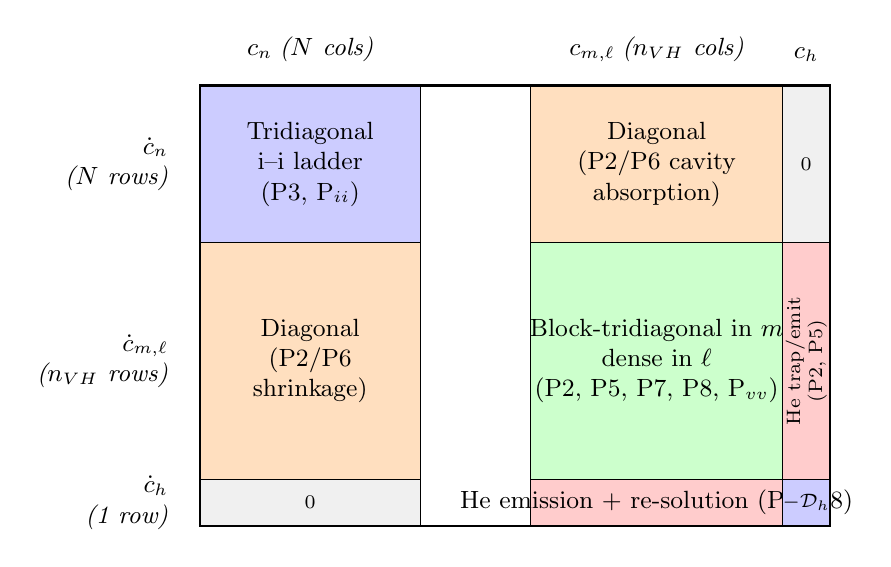
\begin{tikzpicture}[
    block/.style n args={3}{
        draw,
        fill=#1,
        minimum width=#2,
        minimum height=#3,
        inner sep=0pt,
        outer sep=0pt
    },
    mylabel/.style={font=\small\itshape},
    every node/.style={font=\small}
]
% --- block widths/heights (pure numbers, unit cm) ---
\def\wI{2.8}   % SIA column width
\def\wV{3.2}   % VacHe column width
\def\wH{0.6}   % c_h column width
\def\hI{2.0}   % SIA row height
\def\hV{3.0}   % VacHe row height
\def\hH{0.6}   % c_h row height

% Derived x-centres (pure numbers)
\pgfmathsetmacro{\xV}{\wI + 0.5*\wV}       % centre of column 2
\pgfmathsetmacro{\xH}{\wI + \wV + 0.5*\wH} % centre of column 3

% Derived y-centres (pure numbers, negative = downward)
\pgfmathsetmacro{\yII}{-(0.5*\hI + 0.5*\hV)}        % centre of row 2
\pgfmathsetmacro{\yIII}{-(0.5*\hI + \hV + 0.5*\hH)} % centre of row 3

% ---- Row 1: dc_n/dt ----
\node[block={blue!20}{\wI cm}{\hI cm}]
    (A11) at (0, 0) {};
\node[align=center] at (A11.center)
    {Tridiagonal\\i--i ladder\\(P3, P$_{ii}$)};

\node[block={orange!25}{\wV cm}{\hI cm}]
    (A12) at (\xV cm, 0) {};
\node[align=center] at (A12.center)
    {Diagonal\\(P2/P6 cavity\\absorption)};

\node[block={gray!12}{\wH cm}{\hI cm}]
    (A13) at (\xH cm, 0) {};
\node[font=\scriptsize] at (A13.center) {0};

% ---- Row 2: dc_{m,ell}/dt ----
\node[block={orange!25}{\wI cm}{\hV cm}]
    (A21) at (0, \yII cm) {};
\node[align=center] at (A21.center)
    {Diagonal\\(P2/P6\\shrinkage)};

\node[block={green!20}{\wV cm}{\hV cm}]
    (A22) at (\xV cm, \yII cm) {};
\node[align=center] at (A22.center)
    {Block-tridiagonal in $m$\\dense in $\ell$\\(P2, P5, P7, P8, P$_{vv}$)};

\node[block={red!20}{\wH cm}{\hV cm}]
    (A23) at (\xH cm, \yII cm) {};
\node[align=center, font=\scriptsize, rotate=90] at (A23.center)
    {He trap/emit\\(P2, P5)};

% ---- Row 3: dc_h/dt ----
\node[block={gray!12}{\wI cm}{\hH cm}]
    (A31) at (0, \yIII cm) {};
\node[font=\scriptsize] at (A31.center) {0};

\node[block={red!20}{\wV cm}{\hH cm}]
    (A32) at (\xV cm, \yIII cm) {};
\node[align=center] at (A32.center)
    {He emission + re-solution (P5, P8)};

\node[block={blue!20}{\wH cm}{\hH cm}]
    (A33) at (\xH cm, \yIII cm) {};
\node[font=\scriptsize] at (A33.center) {$-\mathcal{D}_h$};

% ---- column labels (above row-1 blocks) ----
\node[mylabel, above=5pt] at (A11.north) {$c_n$\;($N$ cols)};
\node[mylabel, above=5pt] at (A12.north) {$c_{m,\ell}$\;($n_{VH}$ cols)};
\node[mylabel, above=5pt] at (A13.north) {$c_h$};

% ---- row labels (left of column-1 blocks) ----
\node[mylabel, left=8pt, align=right] at (A11.west)
    {$\dot{c}_n$\\($N$ rows)};
\node[mylabel, left=8pt, align=right] at (A21.west)
    {$\dot{c}_{m,\ell}$\\($n_{VH}$ rows)};
\node[mylabel, left=8pt, align=right] at (A31.west)
    {$\dot{c}_h$\\(1 row)};

% ---- outer border ----
\draw[thick] (A11.north west) rectangle (A33.south east);

\end{tikzpicture}
\end{center}

\noindent
The Jacobian $\partial\mathbf{f}/\partial\mathbf{y}$ inherits this block
structure. The blue tridiagonal block (i--i ladder) has bandwidth 2 in $n$.
The green block-tridiagonal (vacancy/He) has block size $(\ell_{\max}+1)$
and tridiagonal coupling in $m$ from P2/P5, with dense $\ell$-coupling
within each block from the He exchange terms P2/P5/P7/P8. The orange
off-diagonal blocks are sparse-diagonal: each $c_n$ couples to all
$\bar{c}_m$ through the cavity absorption rate, and each $c_{m,\ell}$
couples to all $c_n$ through the SIA-shrinkage rate. The red column/row
couples the free-He scalar $c_h$ to every $(m,\ell)$ node.

\paragraph{General coalescence case.}
When cluster--cluster coalescence is included up to the mobility
cutoffs $n_{\max}^i$ and $m_{\max}^v$, the sparsity pattern changes
in three blocks. (i) The SIA--SIA block becomes
\emph{dense lower-triangular} within the $n_{\max}^i \times n_{\max}^i$
mobile sub-block: i--i coalescence couples every pair $(n', n-n')$ with
$n' \leq n_{\max}^i$, filling the lower triangle. Rows $n > n_{\max}^i$
(immobile loops) retain the tridiagonal structure of the mono-defect
case. (ii) The SIA--VacHe and VacHe--SIA cross blocks become \emph{dense
in the mobile strip}: v--i annihilation couples every mobile vacancy
cluster $V_{m'}$ ($m' \leq m_{\max}^v$) to every SIA cluster $I_n$
($n \leq n_{\max}^i$), filling a $n_{\max}^i \times m_{\max}^v$
sub-block. Outside the mobile strips both blocks remain diagonal (the
immobile-cluster interactions are still mono-defect in form). (iii) The
VacHe--VacHe block gains a \emph{dense $m_{\max}^v \times m_{\max}^v$
corner}: v--v coalescence fills the upper-left sub-block corresponding
to the mobile vacancy clusters, on top of the block-tridiagonal
structure inherited from P2/P5/P7/P8.

\begin{center}
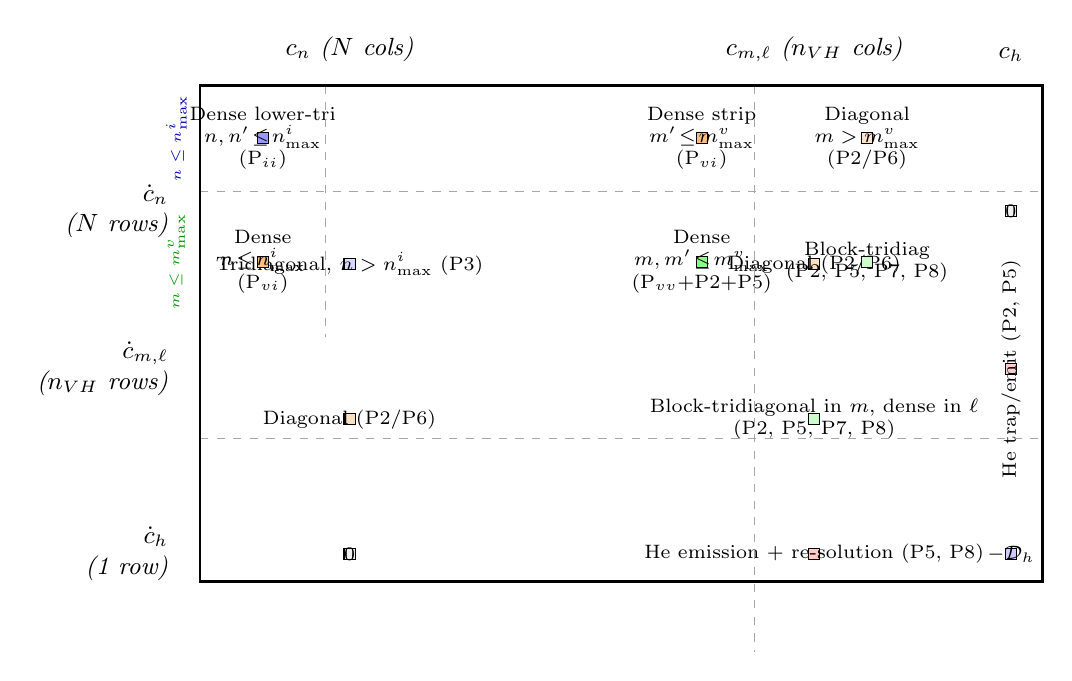
\begin{tikzpicture}[
    x=1cm,y=1cm,
    block/.style n args={3}{
        draw,
        fill=#1,
        minimum width=#2,
        minimum height=#3,
        inner sep=2pt,
        outer sep=0pt
    },
    mylabel/.style={font=\small\itshape},
    every node/.style={font=\small}
]

%========================================================
% Dimensions
%========================================================
\def\wI{3.8}    % SIA column width
\def\wV{4.2}    % VacHe column width
\def\wH{0.8}    % c_h column width
\def\hI{3.2}    % SIA row total height
\def\hV{4.0}    % VacHe row total height
\def\hH{0.7}    % c_h row height

% mobile fractions:  fI = n_max^i / N,  fV = m_max^v / M  (schematic)
\def\fI{0.42}
\def\fV{0.32}

%========================================================
% Derived geometry
%========================================================
\pgfmathsetmacro{\xV}{\wI + 0.5*\wV}
\pgfmathsetmacro{\xH}{\wI + \wV + 0.5*\wH}

\pgfmathsetmacro{\yII}{-(0.5*\hI + 0.5*\hV)}
\pgfmathsetmacro{\yIII}{-(0.5*\hI + \hV + 0.5*\hH)}

\pgfmathsetmacro{\wIm}{\fI*\wI}
\pgfmathsetmacro{\hIm}{\fI*\hI}
\pgfmathsetmacro{\wVm}{\fV*\wV}
\pgfmathsetmacro{\hVm}{\fV*\hV}

\pgfmathsetmacro{\xVm}{\wI + 0.5*\wVm}
\pgfmathsetmacro{\xVi}{\wI + \wVm + 0.5*(\wV-\wVm)}

\pgfmathsetmacro{\yIm}{-0.5*\hIm}
\pgfmathsetmacro{\yIi}{-\hIm - 0.5*(\hI-\hIm)}

\pgfmathsetmacro{\yIIm}{-(0.5*\hI + 0.5*\hVm)}
\pgfmathsetmacro{\yIIi}{-(0.5*\hI + \hVm + 0.5*(\hV-\hVm))}

% x-centre of mobile SIA sub-block: flush left of column 1
\pgfmathsetmacro{\xA}{-0.5*\wI + 0.5*\wIm}
\pgfmathsetmacro{\xLeft}{-0.5*\wI}
\pgfmathsetmacro{\xRight}{\xH + 0.5*\wH}

\pgfmathsetmacro{\xdivI}{\xLeft + \wIm}
\pgfmathsetmacro{\xdivV}{\wI + \wVm}
\pgfmathsetmacro{\ydivI}{-\hIm}
\pgfmathsetmacro{\ydivV}{-\hI - \hVm}
\pgfmathsetmacro{\yBottom}{\yIII - 0.5*\hH}

%========================================================
% Row 1: dc_n/dt
%========================================================

% (1,1a) mobile SIA × mobile SIA — dense lower-triangular
\node[block={blue!40}{{\wIm}}{{\hIm}}]
    (A11m) at (\xA,\yIm) {};
\node[align=center,font=\scriptsize] at (A11m.center)
    {Dense lower-tri\\$n,n'\!\le\!n_{\max}^i$\\(P$_{ii}$)};

% (1,1b) immobile SIA × SIA — tridiagonal, mono-defect
\node[block={blue!15}{{\wI}}{{\hI-\hIm}}]
    (A11i) at (0,\yIi) {};
\node[align=center,font=\scriptsize] at (A11i.center)
    {Tridiagonal, $n>n_{\max}^i$ (P3)};

% (1,2a) mobile SIA rows × mobile VacHe cols — dense strip (v–i)
\node[block={orange!50}{{\wVm}}{{\hIm}}]
    (A12m) at (\xVm,\yIm) {};
\node[align=center,font=\scriptsize] at (A12m.center)
    {Dense strip\\$m'\!\le\!m_{\max}^v$\\(P$_{vi}$)};

% (1,2b) mobile SIA rows × immobile VacHe cols — diagonal
\node[block={orange!20}{{\wV-\wVm}}{{\hIm}}]
    (A12i) at (\xVi,\yIm) {};
\node[align=center,font=\scriptsize] at (A12i.center)
    {Diagonal\\$m>m_{\max}^v$\\(P2/P6)};

% (1,2c) immobile SIA rows × all VacHe cols — diagonal
\node[block={orange!25}{{\wV}}{{\hI-\hIm}}]
    (A12ii) at (\xV,\yIi) {};
\node[align=center,font=\scriptsize] at (A12ii.center)
    {Diagonal (P2/P6)};

% (1,3) SIA × c_h — zero
\node[block={gray!12}{{\wH}}{{\hI}}]
    (A13) at (\xH,{-0.5*\hI}) {};
\node[font=\scriptsize] at (A13.center) {0};

%========================================================
% Row 2: dc_{m,ell}/dt
%========================================================

% (2,1a) mobile VacHe rows × mobile SIA cols — dense (v–i)
\node[block={orange!50}{{\wIm}}{{\hVm}}]
    (A21m) at (\xA,\yIIm) {};
\node[align=center,font=\scriptsize] at (A21m.center)
    {Dense\\$n\!\le\!n_{\max}^i$\\(P$_{vi}$)};

% (2,1b) immobile VacHe rows × SIA cols — diagonal
\node[block={orange!25}{{\wI}}{{\hV-\hVm}}]
    (A21i) at (0,\yIIi) {};
\node[align=center,font=\scriptsize] at (A21i.center)
    {Diagonal (P2/P6)};

% (2,2a) mobile × mobile VacHe — dense corner (v–v + P2/P5)
\node[block={green!45}{{\wVm}}{{\hVm}}]
    (A22m) at (\xVm,\yIIm) {};
\node[align=center,font=\scriptsize] at (A22m.center)
    {Dense\\$m,m'\!\le\!m_{\max}^v$\\(P$_{vv}$+P2+P5)};

% (2,2b) mobile VacHe rows × immobile VacHe cols
\node[block={green!20}{{\wV-\wVm}}{{\hVm}}]
    (A22mi) at (\xVi,\yIIm) {};
\node[align=center,font=\scriptsize] at (A22mi.center)
    {Block-tridiag\\(P2, P5, P7, P8)};

% (2,2c) immobile VacHe — block-tridiagonal in m, dense in ell
\node[block={green!20}{{\wV}}{{\hV-\hVm}}]
    (A22i) at (\xV,\yIIi) {};
\node[align=center,font=\scriptsize] at (A22i.center)
    {Block-tridiagonal in $m$, dense in $\ell$\\(P2, P5, P7, P8)};

% (2,3) VacHe × c_h — He trapping / emission
\node[block={red!20}{{\wH}}{{\hV}}]
    (A23) at (\xH,\yII) {};
\node[align=center,font=\scriptsize,rotate=90] at (A23.center)
    {He trap/emit (P2, P5)};

%========================================================
% Row 3: dc_h/dt  (unchanged from mono-defect)
%========================================================

\node[block={gray!12}{{\wI}}{{\hH}}]
    (A31) at (0,\yIII) {};
\node[font=\scriptsize] at (A31.center) {0};

\node[block={red!20}{{\wV}}{{\hH}}]
    (A32) at (\xV,\yIII) {};
\node[align=center,font=\scriptsize] at (A32.center)
    {He emission + re-solution (P5, P8)};

\node[block={blue!20}{{\wH}}{{\hH}}]
    (A33) at (\xH,\yIII) {};
\node[font=\scriptsize] at (A33.center) {$-\mathcal{D}_h$};

%========================================================
% Column labels (above top edge y = 0)
%========================================================

\node[mylabel,above=5pt] at (0,0)          {$c_n$ ($N$ cols)};
\node[mylabel,above=5pt] at (\xV,0)        {$c_{m,\ell}$ ($n_{VH}$ cols)};
\node[mylabel,above=5pt] at (\xH,0)        {$c_h$};

%========================================================
% Row labels (left of column-1 left edge)
%========================================================

\node[mylabel,left=8pt,align=right] at (\xLeft,{-0.5*\hI})
    {$\dot{c}_n$\\($N$ rows)};
\node[mylabel,left=8pt,align=right] at (\xLeft,\yII)
    {$\dot{c}_{m,\ell}$\\($n_{VH}$ rows)};
\node[mylabel,left=8pt,align=right] at (\xLeft,\yIII)
    {$\dot{c}_h$\\(1 row)};

% Side annotations for mobile sub-block extents
\node[font=\tiny,text=blue!70!black,rotate=90]
    at (\xLeft-0.3,\yIm)  {$n \le n_{\max}^i$};
\node[font=\tiny,text=green!60!black,rotate=90]
    at (\xLeft-0.3,\yIIm) {$m \le m_{\max}^v$};

%========================================================
% Dashed dividers at mobile/immobile boundaries
%========================================================

% vertical: inside SIA column at x = xLeft + wIm
\draw[dashed,gray!70] (\xdivI, 0)         -- (\xdivI, {-\hI});
% vertical: inside VacHe column at x = wI + wVm
\draw[dashed,gray!70] (\xdivV, 0)         -- (\xdivV, {-\hI-\hV});
% horizontal: between mobile/immobile SIA rows at y = -hIm
\draw[dashed,gray!70] (\xLeft, \ydivI)    -- (\xRight, \ydivI);
% horizontal: between mobile/immobile VacHe rows at y = -hI - hVm
\draw[dashed,gray!70] (\xLeft, \ydivV)    -- (\xRight, \ydivV);

%========================================================
% Outer border
%========================================================

\draw[thick] (\xLeft,0) rectangle (\xRight,\yBottom);

\end{tikzpicture}
\end{center}

\noindent
The dashed lines mark the mobile/immobile boundaries at $n = n_{\max}^i$
(vertical, in the SIA blocks) and $m = m_{\max}^v$ (vertical, in the
VacHe blocks; horizontal, separating mobile and immobile vacancy rows).
Darker shading indicates blocks that are denser in the coalescence
formulation than in the mono-defect case. The $c_h$ column and row
(red) and the immobile-cluster sub-blocks (lighter shading) are
structurally identical to the mono-defect diagram above.

%-------------------------------------------------------------------
\subsubsection{He Content and Reduction Approximations}
\label{sec:He_approx}
%-------------------------------------------------------------------

The dominant contributor to system size is the He index $\ell$. The
maximum He loading per cluster grows with cavity size as
\begin{equation}\label{eq:ellmax}
    \ell_{\max}(m) = \lfloor \alpha_{\mathrm{He}}\,m^{2/3} \rfloor,
    \qquad \alpha_{\mathrm{He}} = 1.5\text{--}2.0,
\end{equation}
giving a total vacancy--He grid size
\begin{equation}\label{eq:nVH_full}
    n_{VH}^{\mathrm{full}}
    = \sum_{m=1}^{M}\bigl[\ell_{\max}(m)+1\bigr]
    \approx M + \alpha_{\mathrm{He}}\sum_{m=1}^{M} m^{2/3}
    \approx M\Bigl(1 + \tfrac{3}{5}\alpha_{\mathrm{He}}\,M^{2/3}\Bigr),
\end{equation}
which scales as $M^{5/3}$ and can reach $10^4$--$10^5$ for
$M = 10^3$--$10^4$. Two physics-based approximations reduce this
substantially, exploiting the very different He budgets in fission and
fusion irradiation environments.

\paragraph{Case~1 --- Fusion (high He/dpa): mean-field He approximation.}
Under fusion-relevant He generation rates ($\sim$10--15 appm He/dpa), He
quickly saturates every cavity to its equilibrium loading. The two-dimensional
$(m,\ell)$ distribution can then be collapsed to a one-dimensional problem
by tracking only the mean He loading per cavity size:
\begin{equation}\label{eq:mean_He}
    \bar{\ell}(m,t) \equiv \frac{\sum_\ell \ell\,c_{m,\ell}}{\bar{c}_m},
\end{equation}
and treating the He distribution within each $m$-bin as a delta function
at $\bar{\ell}(m)$. This replaces the $n_{VH}^{\mathrm{full}}$ equations
for $c_{m,\ell}$ with two ODEs per vacancy size --- one for the total
cavity concentration $\bar{c}_m$ and one for the mean He content
$\bar{\ell}_m$ --- plus the single free-He equation:
\begin{equation}\label{eq:nVH_fusion}
    n_{\mathrm{eq}}^{\mathrm{fusion}}
    = N + \underbrace{2M}_{\bar{c}_m,\;\bar{\ell}_m} + \underbrace{1}_{c_h}
    = N + 2M + 1.
\end{equation}

\paragraph{Case~2 --- Fission (low He/dpa): decoupled-He approximation.}
Fission reactors produce $\sim$0.1--1 appm He/dpa, so He loading remains
low ($\ell \ll \ell_{\max}$) and bubbles are rare. Most cavities are pure
voids ($\ell = 0$). He can then be decoupled: track $c_{m,0}$ (pure voids)
separately from a single mean-field He concentration per size, treating
bubble nucleation as a perturbation to the void distribution. In the
simplest implementation this retains one He-bearing species per $m$ and
adds a single free-He equation:
\begin{equation}\label{eq:nVH_fission}
    n_{\mathrm{eq}}^{\mathrm{fission}}
    = N + \underbrace{M}_{\text{voids }c_{m,0}} + \underbrace{1}_{\bar{c}_{m,\ell\geq 1}}
      + \underbrace{1}_{c_h}
    = N + M + 2.
\end{equation}

%-------------------------------------------------------------------
\subsubsection{System Size Summary}
\label{sec:system_size_table}
%-------------------------------------------------------------------

Table~\ref{tab:system_size} collects the ODE counts for typical
parameter choices ($N = 1000$, $M = 1000$, $\alpha_{\mathrm{He}} = 1.5$).

\begin{table}[htbp]
\centering
\caption{ODE system size for the three He-content strategies. All
entries assume $N = 1000$ SIA sizes, $M = 1000$ vacancy sizes,
$\alpha_{\mathrm{He}} = 1.5$, and $n_{\max}^i = 100$, $m_{\max}^v = 5$.
The column ``Dominant block'' identifies the bottleneck for
Jacobian factorisation. Logarithmic size-binning for
$m > m_{\mathrm{group}} \sim 100$--200 can reduce $n_{VH}$ by a further
factor of 3--5.}
\label{tab:system_size}
\renewcommand{\arraystretch}{1.25}
\begin{tabular}{@{}lcccc@{}}
\toprule
\textbf{He strategy} & \textbf{SIA block ($N$)}
  & \textbf{VacHe block ($n_{VH}$)}
  & $\mathbf{n_{\mathrm{eq}}}$
  & \textbf{Dominant block} \\
\midrule
Full $(m,\ell)$ grid (Eq.~\ref{eq:nVH_full})
  & 1\,000 & $\sim$38\,000 & $\sim$39\,001 & VacHe \\
Case~1: mean-field He, fusion (Eq.~\ref{eq:nVH_fusion})
  & 1\,000 & 2\,000 & 3\,001 & SIA + VacHe \\
Case~2: decoupled He, fission (Eq.~\ref{eq:nVH_fission})
  & 1\,000 & 1\,001 & 2\,002 & SIA + VacHe \\
\bottomrule
\end{tabular}
\end{table}

%-------------------------------------------------------------------
\subsubsection{Stiffness and Solver Strategy}
\label{sec:solver}
%-------------------------------------------------------------------

The system~\eqref{eq:state_vector} is severely stiff. The stiffness
ratio is dominated by the disparity between the He migration frequency
and the vacancy frequency,
\begin{equation}\label{eq:stiffness}
    \frac{\omega_h^{\mathrm{eff}}}{\omega_v^{\mathrm{eff}}}
    \sim 10^4\text{--}10^8,
\end{equation}
with additional stiffness contributed by the contrast between
fast mobile-cluster reactions (small $n,m$) and slow large-cluster
dynamics. An implicit solver with adaptive time stepping is mandatory;
recommended options are LSODA (automatic stiffness detection) or CVODE
(variable-order BDF with sparse Jacobian). Practical tolerances are
\texttt{rtol}~$= 10^{-8}$, \texttt{atol}~$= 10^{-12}$ for the
conservation diagnostics of Section~\ref{sec:conservation_check} to
remain below $10^{-6}$.

Logarithmic size-binning (grouping) replaces the uniform $m$-grid with
logarithmically spaced bins for $m > m_{\mathrm{group}} \approx 50$--200.
Each bin $[m_k, m_{k+1})$ is represented by a single representative
concentration; capture rates are evaluated at the bin midpoint and
weighted by the bin width. This reduces $n_{VH}$ by a factor of 3--10
with negligible loss of accuracy for the swelling and loop-density
predictions. The conservation diagnostics should be evaluated at every
output step; the implementation should assert a hard stop if
$\delta_{\mathrm{FP}}$ or $\delta_{\mathrm{He}}$ exceeds $10^{-3}$.

%===================================================================
\section{State Space Reduction via Size-Bin Moments}
\label{sec:size_moments}
%===================================================================

The cluster dynamics (CD) system derived in
Section~\ref{sec:rate_equations} tracks one ODE per cluster size.
Even after the He approximations of Section~\ref{sec:HeV_CD}, the SIA
ladder runs to $N \sim 10^3$--$10^4$ and the vacancy grid to
$M \sim 10^3$--$10^4$, giving several thousand coupled ODEs. For
large-scale parametric studies or coupling to microstructure-informed
continuum codes, a further reduction is desirable. This section
presents a systematic size-grouping framework that replaces the
per-size equations with a much smaller set of \emph{bin moment
equations}, derived by integrating the master equations over
logarithmically spaced size bins. Two closure strategies are described:
a \emph{moment-closure} approach analogous to the method of moments in
aerosol science, and a \emph{shape-function} approach analogous to the
Galerkin finite-element method. Both reduce the ODE count from
$O(N)$ or $O(M)$ to $O(N_B)$ where
$N_B = O(\log N / \log r)$ for bin ratio $r > 1$, typically 20--60
bins for $N = 10^4$ and $r = 1.5$--$2$.

The derivation is presented for the SIA cluster population $c_n$; the
vacancy cluster population $\bar{c}_m$ follows by identical steps with
$n \to m$, $N \to M$, and the appropriate rate constants substituted.

%-------------------------------------------------------------------
\subsection{Logarithmic Bin Partition}
\label{sec:log_bins}
%-------------------------------------------------------------------

Partition the integer size axis $\{1, 2, \ldots, N\}$ into $N_B$ bins.
The first $n_0$ sizes (mobile clusters, $n \leq n_{\max}^i$) are
resolved individually; the remaining large immobile clusters are
grouped. Define the bin boundaries
\begin{equation}\label{eq:bin_boundaries}
    1 = s_0 < s_1 < \cdots < s_{n_0} = n_{\max}^i
    < s_{n_0+1} < \cdots < s_{N_B} = N,
\end{equation}
where for $k > n_0$ the boundaries follow a geometric progression with
ratio $r > 1$:
\begin{equation}\label{eq:bin_ratio}
    s_{k+1} = \lfloor r\,s_k \rfloor + 1,
    \qquad r = 1.5\text{--}2.0.
\end{equation}
Bin $k$ spans the integer interval $\mathcal{B}_k = \{s \in \mathbb{Z}
: s_k \leq s < s_{k+1}\}$ and contains $\Delta_k = s_{k+1} - s_k$
cluster sizes. The representative size of bin $k$ is the geometric
mean of its boundaries:
\begin{equation}\label{eq:shat}
    \hat{s}_k = \sqrt{s_k\,s_{k+1}}.
\end{equation}

The number of grouped bins is
\begin{equation}\label{eq:NB}
    N_B^{\mathrm{group}} = \left\lceil
        \frac{\ln(N/n_{\max}^i)}{\ln r}
    \right\rceil,
    \qquad
    N_B = n_{\max}^i + N_B^{\mathrm{group}}.
\end{equation}
For $N = 5000$, $n_{\max}^i = 100$, $r = 2$: $N_B^{\mathrm{group}}
= \lceil \ln(50)/\ln 2 \rceil = 6$, so only 106 equations replace
4900 per-size ODEs.

%-------------------------------------------------------------------
\subsection{Bin Moments}
\label{sec:bin_moments}
%-------------------------------------------------------------------

For each bin $k$ define the \emph{zeroth moment} (total cluster
concentration in the bin) and the \emph{first moment} (total defect
inventory in the bin):
\begin{equation}\label{eq:bin_moments_def}
    \mu_k^{(0)}(t) \equiv \sum_{n \in \mathcal{B}_k} c_n(t),
    \qquad
    \mu_k^{(1)}(t) \equiv \sum_{n \in \mathcal{B}_k} n\,c_n(t).
\end{equation}
The mean cluster size within bin $k$ is
$\langle n \rangle_k = \mu_k^{(1)}/\mu_k^{(0)}$ and the swelling
(first-moment sum) is $S_I = \sum_k \mu_k^{(1)}$. Higher moments
can be defined similarly; in practice, tracking $(\mu_k^{(0)},
\mu_k^{(1)})$ at each bin is sufficient to close the rate equations
to second order.

%-------------------------------------------------------------------
\subsection{Bin-Integrated Rate Equations}
\label{sec:bin_rate_eq}
%-------------------------------------------------------------------

Summing the master equation~\eqref{eq:ME_SIA} over all $n \in
\mathcal{B}_k$ gives the zeroth-moment equation:
\begin{equation}\label{eq:mu0_eq}
\begin{split}
    \frac{d\mu_k^{(0)}}{dt} = {} &
    \underbrace{
        \sum_{n \in \mathcal{B}_k} G_n
    }_{\text{production}}
    \;+\; \underbrace{
        J_{k-1 \to k} - J_{k \to k+1}
    }_{\substack{\text{inter-bin flux}\\(\text{advection in size space})}}
    \\[4pt]
    &- \underbrace{
        \mu_k^{(0)}\sum_{m=1}^{M}
        \hat{\mathcal{K}}_{k,m}^{(\mathrm{cav})}\,\bar{c}_m
    }_{\text{cavity absorption}}
    \;-\; \underbrace{
        \mathcal{D}_i\,\mu_k^{(0)}
    }_{\text{fixed sinks}}
    \;+\; R_k,
\end{split}
\end{equation}
where $R_k$ collects the emission, coalescence, and trap-mutation
source terms (see below), and $\hat{\mathcal{K}}_{k,m}^{(\mathrm{cav})}$
is the bin-averaged cavity absorption rate:
\begin{equation}\label{eq:Khat}
    \hat{\mathcal{K}}_{k,m}^{(\mathrm{cav})}
    \equiv \frac{1}{\Delta_k}
    \sum_{n \in \mathcal{B}_k}
    \mathcal{K}_{n,m}^{(\mathrm{cav})}.
\end{equation}
The \emph{inter-bin flux} from bin $k$ to bin $k+1$ counts clusters
that grow past the boundary $s_{k+1}$ by absorbing a mono-defect
(or a mobile cluster in the coalescence formulation):
\begin{equation}\label{eq:inter_bin_flux}
    J_{k \to k+1}
    = \hat{\mathcal{K}}_{k,\mathrm{bdy}}^{ii}\,
      \mu_k^{(0)}\,c_{n_{\max}^i}
    + \sum_{m'=1}^{m_{\max}^v}
      \hat{\mathcal{K}}_{k,\mathrm{bdy}}^{vi,m'}\,
      \mu_k^{(0)}\,c_{m',0},
\end{equation}
where $\hat{\mathcal{K}}_{k,\mathrm{bdy}}$ denotes the rate constant
evaluated at the bin boundary $s_{k+1}$. In the mono-defect limit
($n_{\max}^i = m_{\max}^v = 1$), this simplifies to
\begin{equation}\label{eq:Jkk1_monodefect}
    J_{k \to k+1}^{\mathrm{mono}}
    = \mathcal{K}_{i,s_{k+1}}^{\mathrm{loop}}\,c_1\,\mu_k^{(0)},
\end{equation}
i.e.\ the rate at which clusters sitting at the upper boundary of bin
$k$ absorb a mono-SIA and cross into bin $k+1$.

Multiplying Eq.~\eqref{eq:ME_SIA} by $n$ and summing over
$\mathcal{B}_k$ gives the first-moment equation:
\begin{equation}\label{eq:mu1_eq}
\begin{split}
    \frac{d\mu_k^{(1)}}{dt} = {} &
    \sum_{n \in \mathcal{B}_k} n\,G_n
    \;+\; s_{k+1}\,J_{k-1 \to k} - s_k\,J_{k \to k+1}
    \;+\; \mu_k^{(0)}
         \bigl(\hat{\mathcal{K}}_{k}^{ii} - \hat{\mathcal{K}}_{k}^{vi}\bigr)
    \\[4pt]
    &- \mu_k^{(1)}\sum_{m=1}^{M}
        \hat{\mathcal{K}}_{k,m}^{(\mathrm{cav})}\,\bar{c}_m
    - \mathcal{D}_i\,\mu_k^{(1)}
    + n\text{-weighted source terms},
\end{split}
\end{equation}
where the second line accounts for the fact that SIA absorption
increases the size of each cluster by the absorbed cluster's size,
and the inter-bin flux carries the boundary-size weight $s_{k+1}$
(clusters entering bin $k+1$) or $s_k$ (clusters leaving).

%-------------------------------------------------------------------
\subsection{Closure: Two Strategies}
\label{sec:closure}
%-------------------------------------------------------------------

Both $\mu_k^{(0)}$ and $\mu_k^{(1)}$ are known at each time step.
The rate equations above contain products such as
$\hat{\mathcal{K}}_{k,m}^{(\mathrm{cav})} \mu_k^{(0)}$ and
$J_{k\to k+1}$, which require knowledge of the \emph{intra-bin
distribution} $c_n$ for $n \in \mathcal{B}_k$. Two strategies
close this system.

\subsubsection{Piecewise-Constant (Zeroth-Order) Closure}
\label{sec:pc_closure}

Assume the distribution is uniform within each bin:
\begin{equation}\label{eq:pc_ansatz}
    c_n \approx \frac{\mu_k^{(0)}}{\Delta_k}
    \equiv \bar{c}_k
    \qquad \forall\; n \in \mathcal{B}_k.
\end{equation}
Then all bin-averaged rate constants reduce to evaluation at the bin
midpoint $\hat{s}_k$:
\begin{equation}\label{eq:Khat_pc}
    \hat{\mathcal{K}}_{k,m}^{(\mathrm{cav})}
    \approx \mathcal{K}_{\hat{s}_k,m}^{(\mathrm{cav})},
\end{equation}
and the inter-bin flux becomes
\begin{equation}\label{eq:Jkk1_pc}
    J_{k \to k+1}
    \approx \mathcal{K}_{i,\hat{s}_{k+1}}^{\mathrm{loop}}\,
            c_1\,\bar{c}_k.
\end{equation}
This is the standard \emph{logarithmic grouping} used in most
production CD codes~\cite{Golubov2001,Barashev2004}. It conserves
$\mu_k^{(0)}$ exactly but not $\mu_k^{(1)}$; the error in $S_I$ is
$O(\Delta_k/\hat{s}_k) = O(r-1)$.

\subsubsection{Shape-Function (Galerkin) Closure}
\label{sec:fem_closure}

Approximate the intra-bin distribution as a linear combination of
basis functions defined on the bin:
\begin{equation}\label{eq:shape_ansatz}
    c_n \approx \sum_{p} a_k^{(p)}\,\phi_p(n),
    \qquad n \in \mathcal{B}_k,
\end{equation}
where the coefficients $a_k^{(p)}$ are determined by the known
moments $(\mu_k^{(0)}, \mu_k^{(1)}, \ldots)$ and
$\phi_p$ are chosen basis functions on $\mathcal{B}_k$.

\paragraph{Hat-function basis (linear FEM on log scale).}
Map $n \in [s_k, s_{k+1})$ to $\xi = \ln(n/s_k)/\ln r \in [0,1)$
and use piecewise-linear (hat) functions:
\begin{equation}\label{eq:hat_basis}
    \phi_0(\xi) = 1 - \xi, \qquad \phi_1(\xi) = \xi.
\end{equation}
The two coefficients $a_k^{(0)}$ and $a_k^{(1)}$ are fixed by the
two moments $\mu_k^{(0)}$ and $\mu_k^{(1)}$ via:
\begin{align}
    a_k^{(0)}\,I_{00} + a_k^{(1)}\,I_{01} &= \mu_k^{(0)},
    \label{eq:hat_moment0}\\
    a_k^{(0)}\,I_{10} + a_k^{(1)}\,I_{11} &= \mu_k^{(1)},
    \label{eq:hat_moment1}
\end{align}
where $I_{pq} = \sum_{n \in \mathcal{B}_k} n^p\,\phi_q(\ln n/s_k/\ln r)$
are geometry integrals computed once at setup. This two-parameter
ansatz is the FEM analogue of the piecewise-linear representation in
aerosol sectional methods~\cite{Adams2002,Jacobson1994}.

\paragraph{Log-normal basis.}
Alternatively, within each bin assume a log-normal shape:
\begin{equation}\label{eq:lognormal_ansatz}
    c_n \approx \frac{a_k}{\sqrt{2\pi}\,\sigma_k\,n}
    \exp\!\left[-\frac{(\ln n - \mu_k)^2}{2\sigma_k^2}\right],
\end{equation}
with $\mu_k = \ln\langle n\rangle_k$ and $\sigma_k$ determined from
the second moment $\mu_k^{(2)}$. This three-parameter closure
requires tracking one additional moment per bin but captures the
asymmetric, right-skewed distributions typical of nucleation-growth
kinetics.

\paragraph{Galerkin projection.}
Regardless of basis, the Galerkin projection of the master
equation~\eqref{eq:ME_SIA} onto $\phi_p$ over $\mathcal{B}_k$ gives:
\begin{equation}\label{eq:galerkin}
    \sum_{n \in \mathcal{B}_k} \phi_p(n)\,\frac{dc_n}{dt}
    = \sum_{n \in \mathcal{B}_k} \phi_p(n)\,f_n(\mathbf{c}),
\end{equation}
where $f_n$ is the right-hand side of Eq.~\eqref{eq:ME_SIA}. The
left side becomes $\dot{a}_k^{(p)}$ (via the moment relations), and
the right side is expressed in terms of $\{a_k^{(p)}\}$ and the
inter-bin fluxes through the shape ansatz. The resulting ODE system
for the coefficients $\{a_k^{(p)}\}$ is closed and of size
$P \times N_B$ where $P$ is the number of moments per bin ($P = 1$
for piecewise-constant, $P = 2$ for hat-function, $P = 3$ for
log-normal).

%-------------------------------------------------------------------
\subsection{Inter-Bin Flux Treatment}
\label{sec:interbin_flux}
%-------------------------------------------------------------------

The inter-bin flux $J_{k \to k+1}$ requires special care because it
drives mass transfer between bins and must satisfy discrete conservation
exactly. Writing the flux as an upwind scheme in size space:

\begin{equation}\label{eq:flux_upwind}
    J_{k \to k+1} =
    \begin{cases}
        \beta_{s_{k+1}}\,c_{s_{k+1}}^- & \text{if growth} > \text{shrinkage},\\
        \beta_{s_{k+1}}\,c_{s_{k+1}}^+ & \text{if shrinkage} > \text{growth},
    \end{cases}
\end{equation}
where $c_{s_{k+1}}^{\pm}$ denotes the distribution evaluated just
below/above the boundary from within the respective bin, and
$\beta_{s_{k+1}}$ is the net growth rate at the boundary:
\begin{equation}\label{eq:beta}
    \beta_s = \mathcal{K}_{i,s}^{\mathrm{loop}}\,c_1
            - \mathcal{K}_{v,s}^{\mathrm{loop}}\,c_{1,0}
            - \varepsilon_i(s).
\end{equation}
The upwind flux preserves positivity of $\mu_k^{(0)}$ and prevents
spurious oscillations between adjacent bins. For the shape-function
closure, $c_{s_{k+1}}^-$ is evaluated from the intra-bin ansatz at
$n = s_{k+1} - 1$, giving a smooth interpolation.

%-------------------------------------------------------------------
\subsection{Accuracy and Conservation Properties}
\label{sec:moment_accuracy}
%-------------------------------------------------------------------

\paragraph{Mass conservation.}
Summing Eq.~\eqref{eq:mu0_eq} over all bins recovers
$dS_I/dt = d(\sum_k \mu_k^{(1)})/dt$ exactly, provided the inter-bin
fluxes satisfy the telescoping identity:
\begin{equation}\label{eq:flux_telescoping}
    \sum_{k=1}^{N_B}(J_{k-1\to k} - J_{k\to k+1}) = 0
\end{equation}
(boundary terms vanish: $J_{0\to 1} = 0$ and $J_{N_B\to N_B+1} = 0$).
This holds for any consistent flux formula. The swelling identity
$S(t) = S_I(t) + \Delta J^d(t)$ (Eq.~\ref{eq:swelling_identity})
therefore remains exact regardless of the grouping scheme.

\paragraph{Truncation error.}
For the piecewise-constant closure (Eq.~\ref{eq:pc_ansatz}), the
error in the bin-averaged rate constant scales as:
\begin{equation}\label{eq:truncation_error}
    \hat{\mathcal{K}}_{k,m}^{(\mathrm{cav})} - \mathcal{K}_{\hat{s}_k,m}^{(\mathrm{cav})}
    = O\!\left(\frac{\Delta_k^2}{\hat{s}_k^2}\right)
    = O\!\left((r-1)^2\right),
\end{equation}
since $\mathcal{K}_{\hat{s},m}^{(\mathrm{cav})} \propto \hat{s}^{1/3}$
or $\hat{s}^{1/2}$ and the bin width scales as $\Delta_k \sim (r-1)\hat{s}_k$.
For $r = 2$ this gives $\sim$25\% error per bin; for $r = 1.5$,
$\sim$6\%. The hat-function closure reduces the error by one order:
$O((r-1)^3)$, making $r = 2$ already accurate to $\lesssim 1\%$.

\paragraph{Moment diagnostics.}
The bin-integrated conservation diagnostics follow from
Section~\ref{sec:conservation_check}:
\begin{equation}\label{eq:delta_FP_binned}
    \delta_{\mathrm{FP}}^{\mathrm{bin}}
    = \frac{\bigl|S - \sum_k\mu_k^{(1)} - \Delta J^d\bigr|}
           {S + \sum_k\mu_k^{(1)} + \Delta J^d},
\end{equation}
which should remain below $10^{-6}$ regardless of binning. A value
above $10^{-4}$ indicates that the inter-bin fluxes are not conserving
mass, typically due to an inconsistent upwind scheme at the bin
boundaries.

%-------------------------------------------------------------------
\subsection{Reduced System Size}
\label{sec:reduced_size}
%-------------------------------------------------------------------

Table~\ref{tab:reduced_size} summarises the ODE count for the
combined He-approximation and size-grouping reductions for
representative parameter choices.

\begin{table}[htbp]
\centering
\caption{ODE counts after combined size-grouping ($r = 2$) and
He-approximation reductions. $P$ is the number of moments per bin
(1 = piecewise-constant, 2 = hat-function). Parameters:
$N = M = 5000$, $n_{\max}^i = 100$, $m_{\max}^v = 5$,
$\alpha_{\mathrm{He}} = 1.5$. ``Full'' refers to the un-grouped
per-size system after He reduction.}
\label{tab:reduced_size}
\renewcommand{\arraystretch}{1.25}
\begin{tabular}{@{}llccc@{}}
\toprule
\textbf{He approx.} & \textbf{Size grouping}
  & $\mathbf{N_B^{SIA}}$
  & $\mathbf{N_B^{vac}}$
  & $\mathbf{n_{\mathrm{eq}}}$ \\
\midrule
Case~1 (fusion) & Full per-size
  & 5\,000 & 10\,000 & 15\,001 \\
Case~1 (fusion) & Log-group, $P=1$
  & 113 & 113 & $226\,P + 1 = 227$ \\
Case~1 (fusion) & Log-group, $P=2$
  & 113 & 113 & $226\,P + 1 = 453$ \\
Case~2 (fission) & Full per-size
  & 5\,000 & 5\,000 & 10\,002 \\
Case~2 (fission) & Log-group, $P=1$
  & 113 & 113 & $226 + 2 = 228$ \\
Case~2 (fission) & Log-group, $P=2$
  & 113 & 113 & $452 + 2 = 454$ \\
\bottomrule
\end{tabular}
\end{table}

\noindent
The log-grouping with $P=1$ reduces the system by a factor of
$\sim$40--70 relative to the per-size He-reduced system, and by a
factor of $\sim$100--200 relative to the full $(m,\ell)$ grid. With
$P=2$ (hat-function), accuracy improves substantially at the cost of
doubling the ODE count, still representing a $\sim$30--100$\times$
reduction. Timing benchmarks on typical irradiation histories
(100 dpa at $10^{-6}$ dpa/s) show that the grouped systems run in
seconds to minutes on a single core, compared with hours for the
full per-size system.

%-------------------------------------------------------------------
\subsection{Implementation Notes}
\label{sec:grouping_impl}
%-------------------------------------------------------------------

\paragraph{Setup.}
At initialisation, precompute: (i) the bin boundaries $\{s_k\}$
from Eq.~\eqref{eq:bin_ratio}; (ii) the representative sizes
$\{\hat{s}_k\}$ from Eq.~\eqref{eq:shat}; (iii) the bin-averaged
rate constants $\hat{\mathcal{K}}_{k,m}^{(\mathrm{cav})}$ for all
$(k,m)$ pairs from Eq.~\eqref{eq:Khat_pc} (piecewise-constant) or
by exact quadrature (hat-function); and (iv) the geometry integrals
$I_{pq}$ for the shape-function closure. Steps (i)--(iv) are
$O(N_B \cdot M)$ and negligible compared with the ODE integration
cost.

\paragraph{Coalescence terms.}
For the i--i coalescence bins, the gain term
$\frac{1}{2}\sum_{n'\in\mathcal{B}_{k'}} \sum_{n''\in\mathcal{B}_{k''}}
\mathcal{K}_{n',n''}^{ii}\,c_{n'}\,c_{n''}$ where $n'+n''\in\mathcal{B}_k$
is approximated as
\begin{equation}\label{eq:coal_binned}
    \frac{1}{2}\,\mathcal{K}_{\hat{s}_{k'},\hat{s}_{k''}}^{ii}\,
    \mu_{k'}^{(0)}\,\mu_{k''}^{(0)}\,
    f_{\mathrm{overlap}}(k,k',k''),
\end{equation}
where $f_{\mathrm{overlap}}$ is the fraction of $(\hat{s}_{k'} +
\hat{s}_{k''})$ that falls within $\mathcal{B}_k$ (a geometric
factor computed at setup). The double sum over bin pairs reduces
from $O(N^2)$ to $O(N_B^2)$, a further speedup of
$(N/N_B)^2 \sim 10^3$--$10^4$.

\paragraph{Coupling to the vacancy grid.}
The SIA bins couple to the vacancy grid through the cavity absorption
term $\hat{\mathcal{K}}_{k,m}^{(\mathrm{cav})}$, which is a
$N_B \times M$ matrix precomputed at setup. When the vacancy grid is
also grouped, this becomes a $N_B^{SIA} \times N_B^{vac}$ matrix,
reducing the coupling cost from $O(N \cdot M)$ to
$O(N_B^{SIA} \cdot N_B^{vac})$ per right-hand-side evaluation.

\paragraph{Conservation check.}
Use Eq.~\eqref{eq:delta_FP_binned} at every output step. An
inconsistency in $\delta_{\mathrm{FP}}^{\mathrm{bin}}$ that was not
present in the ungrouped system localises the error to the inter-bin
flux implementation.


%===================================================================

The full master equation~\eqref{eq:ME_vac} tracks every $(m,\ell)$
pair with $1 \leq m \leq M$ and $0 \leq \ell \leq \ell_{\max}(m)$
(Eq.~\ref{eq:ellmax}), yielding $n_{VH}^{\mathrm{full}}$ coupled ODEs
(Eq.~\ref{eq:nVH_full}) --- typically $10^4$--$10^5$ equations. Two
physics-based approximations exploit the separation of timescales
between He and vacancy kinetics to reduce this to a tractable system.
Both retain the full SIA population (Eq.~\ref{eq:ME_SIA}) and the free
He balance (Eq.~\ref{eq:ME_He}) unchanged; only the vacancy-cluster
block is replaced.

Throughout this section we use the notation and rate constants
established in Sections~\ref{sec:reaction_rates}--\ref{sec:rate_equations}:
$\omega_\alpha^{\mathrm{eff}}$ are the effective reaction frequencies
(Eq.~\ref{eq:omega_eff}); $A_{\mathrm{sph}} = (48\pi^2)^{1/3}$;
$\bar{c}_m = \sum_\ell c_{m,\ell}$ is the total cavity concentration;
and $\mathcal{K}_{n,m}^{(\mathrm{cav})}$ is the SIA-cluster absorption
rate (Eq.~\ref{eq:K_cav}). The vacancy net-flux from size $m$ to $m+1$
is defined as:
\begin{equation}\label{eq:Jv}
    J_{m \to m+1}
    \equiv A_{\mathrm{sph}}\,m^{1/3}\,\omega_v^{\mathrm{eff}}\,
           c_{1,0}\,\bar{c}_m
         - \varepsilon_v(m{+}1,\bar{\ell}(m{+}1))\,\bar{c}_{m+1},
\end{equation}
with forward (capture) and backward (emission) components
$J_{m\to m+1}^{+}$ and $J_{m\to m+1}^{-}$ respectively, so that
$J_{m\to m+1} = J_{m\to m+1}^{+} - J_{m+1\to m}^{-}$.

%===================================================================
\subsection{Case 1: Fast He Equilibration --- Fusion Conditions}
\label{sec:case1}
%===================================================================

At temperatures where vacancies are mobile ($T \gtrsim 200\,^\circ$C),
the He reaction frequency greatly exceeds the vacancy reaction
frequency, $\omega_h^{\mathrm{eff}} \gg \omega_v^{\mathrm{eff}}$.
Helium equilibrates on each cavity faster than the cavity grows or
shrinks, so the full two-dimensional $(m,\ell)$ distribution can be
collapsed to two scalar quantities per vacancy size: the total cavity
concentration $\bar{c}_m$ and the mean He loading
\begin{equation}\label{eq:lbar_def}
    \bar{\ell}(m,t)
    \equiv \frac{\sum_\ell \ell\,c_{m,\ell}}{\bar{c}_m}.
\end{equation}
This is the mean-field He approximation defined in
Eq.~\eqref{eq:mean_He}.

\paragraph{Cavity size distribution.}
Summing Eq.~\eqref{eq:ME_vac} over all $\ell$ at fixed $m$:
\begin{equation}\label{eq:case1_cm}
    \frac{d\bar{c}_m}{dt}
    = J_{m-1 \to m} - J_{m \to m+1}
    - \sum_{n=1}^{n_{\max}^i}
      \mathcal{K}_{n,m}^{(\mathrm{cav})}\,c_n\,\bar{c}_m
    + \Gamma_{\mathrm{TM}}(m{-}1,\bar{\ell})\,\bar{c}_{m-1}
    - \Gamma_{\mathrm{TM}}(m,\bar{\ell})\,\bar{c}_m,
\end{equation}
where the vacancy net flux $J_{m\to m+1}$ is given by
Eq.~\eqref{eq:Jv}. The SIA-shrinkage sum $\sum_n
\mathcal{K}_{n,m}^{(\mathrm{cav})} c_n$ spans all mobile SIA clusters
$n = 1,\ldots,n_{\max}^i$ with no bias factor (spherical cavities are
unbiased, $Z_i^{\mathrm{cav}} = 1$, Eq.~\ref{eq:P2}). The vacancy
capture rate $A_{\mathrm{sph}}\,m^{1/3}\,\omega_v^{\mathrm{eff}}$ is
independent of $\ell$, so the $\ell$-summation is exact for the capture
terms. The emission rate $\varepsilon_v$ depends on $\ell$ through the
He gas-pressure correction to $E_b^v(m,\ell)$ and is approximated by
evaluation at the mean loading $\bar{\ell}(m)$.

\paragraph{Mean He loading.}
Define the He inventory at vacancy size $m$ as
$N_{\mathrm{He}}(m) \equiv \bar{\ell}(m)\,\bar{c}_m$.
Multiplying Eq.~\eqref{eq:ME_vac} by $\ell$, summing over $\ell$, and
collecting terms:
\begin{equation}\label{eq:case1_NHe}
\begin{split}
    \frac{dN_{\mathrm{He}}(m)}{dt} = {} &
      A_{\mathrm{sph}}\,m^{1/3}\,\omega_h^{\mathrm{eff}}\,
      c_h\,\bar{c}_m
    - \varepsilon_h(m,\bar{\ell})\,\bar{c}_m
    - b_0\,\dot{\phi}\,N_{\mathrm{He}}(m)
    \\[3pt]
    &+ \bar{\ell}(m{-}1)\,J_{m-1 \to m}^{+}
     - \bar{\ell}(m)\,J_{m \to m+1}^{+}
    \\
    &+ \bar{\ell}(m{+}1)\,J_{m+1 \to m}^{-}
     - \bar{\ell}(m)\,J_{m \to m-1}^{-}
    \\[3pt]
    &- \bar{\ell}(m)\,
       \sum_{n=1}^{n_{\max}^i}
       \mathcal{K}_{n,m}^{(\mathrm{cav})}\,c_n\,\bar{c}_m.
\end{split}
\end{equation}
The four groups of terms are: (i) He capture from the free pool minus
thermal He emission (P5) minus radiation re-solution (P8); (ii--iii) He
advected in and out as clusters grow or shrink along the $m$-axis,
where $J^+$ is the forward (capture) component and $J^-$ is the
backward (emission) component of the vacancy flux; and (iv) He carried
away when SIA clusters annihilate vacancies. Note the absence of any
bias factor in the SIA-shrinkage term: the rate constant
$\mathcal{K}_{n,m}^{(\mathrm{cav})}$ already encodes the unbiased
cavity geometry ($Z_i^{\mathrm{cav}} = 1$).

Applying the quotient rule
$d\bar{\ell}/dt = (\dot{N}_{\mathrm{He}} - \bar{\ell}\,\dot{\bar{c}}_m)
/ \bar{c}_m$ and substituting Eq.~\eqref{eq:case1_cm}:
\begin{equation}\label{eq:case1_lbar}
\boxed{
\begin{split}
    \frac{d\bar{\ell}(m)}{dt} = {} &
      A_{\mathrm{sph}}\,m^{1/3}\,\omega_h^{\mathrm{eff}}\,c_h
    - \varepsilon_h\bigl(m,\bar{\ell}(m)\bigr)
    - b_0\,\dot{\phi}\,\bar{\ell}(m)
    \\[3pt]
    &+ \frac{J_{m-1 \to m}^{+}}{\bar{c}_m}
       \bigl[\bar{\ell}(m{-}1) - \bar{\ell}(m)\bigr]
     + \frac{J_{m+1 \to m}^{-}}{\bar{c}_m}
       \bigl[\bar{\ell}(m{+}1) - \bar{\ell}(m)\bigr].
\end{split}
}
\end{equation}
Line~1 contains the local He kinetics: trapping from the free pool
(proportional to $c_h$), thermal emission $\varepsilon_h$ (P5,
Eq.~\ref{eq:P5h}), and athermal re-solution (P8, Eq.~\ref{eq:P8})
which drives $\bar{\ell}$ toward zero. Line~2 contains advection
corrections: cavities flowing into size class $m$ carry their own He
loading, which may differ from $\bar{\ell}(m)$; the difference
$[\bar{\ell}(m\pm 1) - \bar{\ell}(m)]$ acts as a drift source.

\paragraph{Numerical implementation.}
In practice, $N_{\mathrm{He}}(m) = \bar{\ell}(m)\,\bar{c}_m$ and
$\bar{c}_m$ are evolved as primary variables; $\bar{\ell}(m)$ is
recovered by division and used only when evaluating rates. When
$\bar{c}_m$ approaches zero near the nucleation threshold, the quotient
becomes ill-conditioned. Recommended practice: set a floor
$\bar{c}_m^{\min} \sim 10^{-30}$\,at/at below which $\bar{\ell}$ is
reset to zero.

\paragraph{Case~1 summary.}
Replacing the full $(m,\ell)$ grid with $2M$ ODEs --- $M$ for
$\bar{c}_m$ (Eq.~\ref{eq:case1_cm}) and $M$ for $\bar{\ell}(m)$
(Eq.~\ref{eq:case1_lbar}) --- plus the unchanged free-He equation
(Eq.~\ref{eq:ME_He}) gives the reduced system count of
Eq.~\eqref{eq:nVH_fusion}:
\begin{equation*}
    n_{\mathrm{eq}}^{\mathrm{fusion}} = N + 2M + 1.
\end{equation*}
The reduction factor relative to the full grid is approximately
$n_{VH}^{\mathrm{full}} / (2M) \approx \tfrac{3}{10}\alpha_{\mathrm{He}}
M^{2/3}$, which is $\sim$10--20 for $M = 10^3$ and
$\alpha_{\mathrm{He}} = 1.5$.

%===================================================================
\subsection{Case 2: Decoupled He Inventory --- Fission Conditions}
\label{sec:case2}
%===================================================================

Under fission irradiation the He generation rate is low
($\sim$0.3--1\,appm/dpa vs.\ $\sim$10--15\,appm/dpa for fusion), so
most cavities carry $\ell \ll m$ and the He/V ratio $\bar{\ell}/m \ll 1$.
Helium acts as a weak perturbation on the void kinetics rather than
controlling nucleation. Rather than tracking $\bar{\ell}(m)$ as a
separate variable at each size, the total trapped He inventory is
followed as a single scalar and distributed algebraically across cavity
sizes.

\paragraph{Cavity size distribution.}
The $\bar{c}_m$ equation is identical to Case~1,
Eq.~\eqref{eq:case1_cm}, with the vacancy emission rate evaluated using
an He-corrected binding energy. In the low-loading limit the He gas
pressure obeys the ideal-gas law, giving an effective binding energy:
\begin{equation}\label{eq:Ebv_eff}
    E_b^{v,\mathrm{eff}}(m)
    \equiv E_b^v\bigl(m,\,\ell(m)\bigr)
    = E_f^v + \frac{2\gamma_s\,\Omega}{r_m}
    - \frac{\ell(m)\,k_BT}{m},
\end{equation}
where $r_m = \xi(m)\,a$, $\gamma_s$ is the surface tension,
$\Omega = a^3/2$ is the atomic volume, and $\ell(m)$ is the He content
assigned to cavities of size $m$ by the allocation rule below. The
third term is the ideal-gas pressure correction $p(\ell,m)\,\Omega =
(\ell\,k_BT/m)\cdot m/m = \ell k_BT/m$, adequate when $\ell/m \ll 1$.
At fission temperatures and low He loading, thermal He emission is
negligible ($E_B^{\mathrm{He}} \gtrsim 2$\,eV); re-solution is the
sole He release channel.

\paragraph{Total trapped He inventory.}
Define $\ell_{\mathrm{tot}} \equiv \sum_{m=1}^M \ell(m)\,\bar{c}_m$.
Summing the He content over all cavities and using
Eq.~\eqref{eq:ME_He} with thermal emission dropped:
\begin{equation}\label{eq:case2_ltot}
    \frac{d\ell_{\mathrm{tot}}}{dt}
    = A_{\mathrm{sph}}\,\omega_h^{\mathrm{eff}}\,c_h
      \sum_{m=1}^{M} m^{1/3}\,\bar{c}_m
    - b_0\,\dot{\phi}\,\ell_{\mathrm{tot}}.
\end{equation}
The first term is the total He trapping rate by all cavities (the sum
is the weighted capture cross-section $\sum_m m^{1/3}\bar{c}_m$), and
the second is the athermal re-solution loss (P8).

\paragraph{He allocation.}
Helium is distributed across cavity sizes in proportion to the capture
rate $A_{\mathrm{sph}}\,m^{1/3}\,\omega_h^{\mathrm{eff}}$, since that
is what determines steady-state He loading when trapping and re-solution
balance:
\begin{equation}\label{eq:allocation}
    \ell(m)
    = \ell_{\mathrm{tot}}\,
      \frac{m^{1/3}\,\bar{c}_m}
           {\displaystyle\sum_{m'=1}^{M} m'^{1/3}\,\bar{c}_{m'}}.
\end{equation}
This algebraic relation is recomputed at each time step. The
$m^{1/3}$ weighting arises from the spherical-cavity capture radius
$\xi(m) \propto m^{1/3}$ (Section~\ref{sec:K3D}), consistent with
$\mathcal{K}_{h,m} = A_{\mathrm{sph}}\,m^{1/3}\,\omega_h^{\mathrm{eff}}$
(Table~\ref{tab:rate_summary}).

\paragraph{Free He.}
The free-He equation retains all terms from Eq.~\eqref{eq:ME_He},
including the fixed-sink loss $\mathcal{D}_h c_h$, but with thermal
He emission dropped:
\begin{equation}\label{eq:case2_ch}
    \frac{dc_h}{dt}
    = G_{\mathrm{He}}
    - A_{\mathrm{sph}}\,\omega_h^{\mathrm{eff}}\,c_h
      \sum_{m=1}^{M} m^{1/3}\,\bar{c}_m
    + b_0\,\dot{\phi}\,\ell_{\mathrm{tot}}
    - \mathcal{D}_h\,c_h.
\end{equation}
The trapping and re-solution terms are exactly the negatives of those
in Eq.~\eqref{eq:case2_ltot}, so the He conservation law
$d(c_h + \ell_{\mathrm{tot}})/dt = G_{\mathrm{He}} - \mathcal{D}_h c_h$
holds (cf.\ Eq.~\ref{eq:dSHe_exact}).

\paragraph{Case~2 summary.}
The reduced system comprises $M$ ODEs for $\bar{c}_m$, one ODE for
$c_h$ (Eq.~\ref{eq:case2_ch}), one ODE for $\ell_{\mathrm{tot}}$
(Eq.~\ref{eq:case2_ltot}), and the algebraic allocation
(Eq.~\ref{eq:allocation}), giving the system count of
Eq.~\eqref{eq:nVH_fission}:
\begin{equation*}
    n_{\mathrm{eq}}^{\mathrm{fission}} = N + M + 2.
\end{equation*}

%===================================================================
\subsection{Radiation Re-Solution: Limiting Behaviour}
\label{sec:resolution_limits}
%===================================================================

The re-solution rate $\Gamma_{\mathrm{res}}(m,\ell) = b_0\,\ell\,\dot{\phi}$
(P8, Eq.~\ref{eq:P8}) is athermal and appears in both reduced models as
$-b_0\,\dot{\phi}\,\bar{\ell}$ in Eq.~\eqref{eq:case1_lbar} and as
$-b_0\,\dot{\phi}\,\ell_{\mathrm{tot}}$ in Eq.~\eqref{eq:case2_ltot}.
Its competition with thermal He emission determines two limiting regimes.

\paragraph{Low-temperature limit ($\varepsilon_h \to 0$).}
Setting $d\bar{\ell}/dt = 0$ in Eq.~\eqref{eq:case1_lbar} and
neglecting the advection terms:
\begin{equation}\label{eq:lbar_ss_lowT}
    \bar{\ell}_{\mathrm{ss}}
    = \frac{A_{\mathrm{sph}}\,m^{1/3}\,\omega_h^{\mathrm{eff}}\,c_h}
           {b_0\,\dot{\phi}}.
\end{equation}
Re-solution sets the equilibrium He loading by competing with trapping.
Without re-solution ($b_0 = 0$), $\bar{\ell}$ grows until
$\ell_{\max}(m)$ is reached.

\paragraph{High-temperature limit
($\varepsilon_h \gg b_0\,\dot{\phi}\,\bar{\ell}$).}
\begin{equation}\label{eq:lbar_ss_highT}
    \bar{\ell}_{\mathrm{ss}}
    \approx \frac{A_{\mathrm{sph}}\,m^{1/3}\,\omega_h^{\mathrm{eff}}\,c_h}
                 {\varepsilon_h(m,\bar{\ell}_{\mathrm{ss}})},
\end{equation}
which is the thermodynamic (detailed-balance) equilibrium loading
(cf.\ Eq.~\ref{eq:P5h}), independent of irradiation rate.

\paragraph{Crossover temperature.}
The transition between the two regimes occurs when
$\varepsilon_h(m,\bar{\ell}) \sim b_0\,\dot{\phi}\,\bar{\ell}$. For
typical EUROFER parameters ($E_B^{\mathrm{He}} \sim 2.0$\,eV,
$b_0 \sim 10^{-2}$\,dpa$^{-1}$, $\dot{\phi} \sim 10^{-6}$\,dpa/s),
this crossover lies at $T \approx 500$--$700\,^\circ$C: below this
temperature re-solution controls He loading; above it thermal emission
dominates.

\paragraph{Consequences for bubble nucleation.}
Re-solution suppresses nucleation at low temperatures by ejecting He
from small embryos, creating an incubation dose $\propto 1/G_{\mathrm{He}}$
for fixed $b_0$. It preferentially dissolves small, He-rich embryos
(low $\ell_{\mathrm{ss}}$ from Eq.~\ref{eq:lbar_ss_lowT}) while leaving
large stable bubbles intact (higher capture rate $\propto m^{1/3}$),
producing the bimodal cavity size distributions commonly observed
experimentally.

%===================================================================
\subsection{Comparison of Cases 1 and 2}
\label{sec:comparison}
%===================================================================

Table~\ref{tab:HeV_comparison} summarises the two approximations and
their applicability. Both use the same $\bar{c}_m$ equation
(Eq.~\ref{eq:case1_cm}) and the same unbiased SIA-shrinkage rate
$\sum_n \mathcal{K}_{n,m}^{(\mathrm{cav})} c_n$; they differ in how
the He degree of freedom is represented and in the approximations made
for thermal He emission. For large $M$, logarithmic size grouping for
$m > m_{\mathrm{group}} \approx 50$--200 is applied in both cases; the
$\bar{\ell}(m)$ variable extends naturally to grouped bins by carrying
the mean loading per bin.

\begin{table}[htbp]
\centering
\caption{Comparison of the two He--vacancy state-space reductions.
Both cases retain the full SIA equation (Eq.~\ref{eq:ME_SIA}) and use
the unbiased cavity absorption rate $\mathcal{K}_{n,m}^{(\mathrm{cav})}$
(Eq.~\ref{eq:K_cav}) with $Z_i^{\mathrm{cav}}=1$.}
\label{tab:HeV_comparison}
\renewcommand{\arraystretch}{1.2}
\begin{tabular}{@{}lcc@{}}
\toprule
& \textbf{Case~1 (Fusion)} & \textbf{Case~2 (Fission)} \\
\midrule
He generation rate & $\sim$10--15\,appm/dpa & $\sim$0.3--1\,appm/dpa \\
Typical He/V ratio $\bar{\ell}/m$ & 0.1--10 & $\ll 1$ \\
He tracked as & $\bar{\ell}(m)$ per size (ODE) & $\ell_{\mathrm{tot}}$ (scalar ODE) \\
He allocation & implicit in $\bar{\ell}(m)$ & algebraic (Eq.~\ref{eq:allocation}) \\
He emission & thermal + re-solution & re-solution only \\
He effect on $E_b^v$ & full $E_b^v(m,\bar{\ell})$ & ideal-gas correction \\
He conservation & Eq.~\ref{eq:mass_He} exactly & Eq.~\ref{eq:dSHe_exact} (approx.) \\
Total ODEs & $N + 2M + 1$ & $N + M + 2$ \\
Reduction vs.\ full grid & $\approx \tfrac{3}{10}\alpha_{\mathrm{He}} M^{2/3}$ & $\approx \tfrac{3}{5}\alpha_{\mathrm{He}} M^{2/3}$ \\
\bottomrule
\end{tabular}
\end{table}

%===================================================================
\section{Extended Cluster Dynamics Model for H, He, V, and I Clusters}
\label{sec:H_extended}
%===================================================================

The foregoing sections treated the irradiated microstructure as a
three-component system: SIA clusters, He--vacancy clusters, and free He.
Under fusion-relevant conditions --- and especially for accelerator-driven
systems where the hydrogen transmutation rate can reach
$\sim$1000--1500\,appm/dpa --- hydrogen must be promoted to an explicit
fourth species.  The key physical differences from helium are:
\begin{enumerate}
  \item H migrates $\sim10^3$--$10^5\times$ faster than vacancies and
        $\sim$10--100$\times$ faster than interstitial He (migration
        energy $E_m^H \approx 0.04$--0.09\,eV versus
        $E_m^{\mathrm{He}} \approx 0.06$--0.13\,eV and
        $E_m^v \approx 0.60$--0.70\,eV in bcc Fe).
  \item H binds to vacancies moderately strongly ($E_b^H \approx
        0.43$--0.57\,eV for H$_n$V$_1$ with $n \leq 6$), so it is
        retained by irradiation-induced vacancies far longer than its
        thermal residence time in the perfect lattice.
  \item H has negligible binding to SIA clusters
        ($E_b^{H\text{-SIA}} \lesssim 0.1$\,eV), so H--SIA clusters
        are treated as unstable and dissociate immediately.
  \item H occupies the \emph{surface shell} of He--V bubbles, forming a
        core-shell He(inside)--H(outside) structure with binding energy
        $E_b^{H\text{-bub}} \approx 0.4$--0.8\,eV.  Up to $\sim m^{2/3}$
        H atoms can be accommodated on the bubble surface.
  \item Because $\omega_H \gg \omega_v$, H equilibrates on every defect
        much faster than the vacancy microstructure evolves.  This
        timescale separation enables an \emph{adiabatic elimination} of
        the H degree of freedom for large clusters, replacing explicit H
        tracking with an algebraic quasi-static loading, exactly as He
        was eliminated in the mean-field approximations of
        Sections~\ref{sec:case1}--\ref{sec:case2}.
\end{enumerate}

The strategy therefore has two tiers:
\begin{description}
  \item[Small clusters ($m \leq m_H^*$, $\ell \leq \ell_H^*$):]
        H is tracked explicitly as an additional cluster index $p$ (number
        of H atoms per cluster), giving a three-dimensional state
        $(m, \ell, p)$ for vacancy-containing clusters.
  \item[Large clusters ($m > m_H^*$):]
        H is adiabatically eliminated; only the \emph{mean H loading}
        $\bar{p}(m,\ell,t)$ per vacancy/He-vacancy cluster is tracked,
        determined at each timestep by the quasi-static condition
        $d\bar{p}/dt = 0$.
\end{description}
The crossover sizes $m_H^* \approx 3$--5 and $\ell_H^* \approx 2$--4
are chosen to cover the clusters whose H-loading dynamics are comparable
to the cluster growth timescale.

%-------------------------------------------------------------------
\subsection{Cluster Notation and State Space}
\label{sec:H_notation}
%-------------------------------------------------------------------

With hydrogen included, the cluster population is extended as follows:

\begin{itemize}
  \item $c_{n}$: concentration of $n$-SIA cluster (loop).
        H binding to SIAs is negligible; this population is unchanged.
  \item $c_{m,\ell,p}$: concentration of a cluster containing
        $m$ vacancies, $\ell$ He atoms, and $p$ H atoms,
        for $m = 1, \ldots, M$; $0 \leq \ell \leq \ell_{\max}(m)$;
        $0 \leq p \leq p_{\max}(m)$.
  \item $c_H$: concentration of free interstitial hydrogen.
  \item $c_h$: concentration of free interstitial helium (unchanged).
\end{itemize}

The maximum H loading per cluster scales with the available surface sites:
\begin{equation}\label{eq:pmax}
    p_{\max}(m) = \lfloor \alpha_H\,m^{2/3} \rfloor,
    \qquad \alpha_H \approx 1.0\text{--}2.0.
\end{equation}
This is identical in form to $\ell_{\max}(m) = \lfloor \alpha_{\mathrm{He}}
m^{2/3} \rfloor$ (Eq.~\ref{eq:ellmax}), reflecting the same surface-area
scaling.

The full three-dimensional $(m,\ell,p)$ state space scales as
\begin{equation}
    n_{VHHe}^{\mathrm{full}}
    \approx M\Bigl(1 + \tfrac{3}{5}\alpha_{\mathrm{He}}\,M^{2/3}\Bigr)
             \cdot \tfrac{1}{2}\bigl(1 + \alpha_H\,M^{2/3}\bigr),
\end{equation}
which grows as $M^{7/3}$ and is intractable for $M \gtrsim 100$.
The adiabatic elimination below reduces this back to the manageable
$(m,\ell)$ plus one extra scalar per $(m,\ell)$ cluster.

%-------------------------------------------------------------------
\subsection{New Reaction Processes Involving Hydrogen}
\label{sec:H_reactions}
%-------------------------------------------------------------------

The existing processes P1--P8 are retained unchanged.  Six new reaction
processes describe H kinetics.

\paragraph{P9: H trapping by a vacancy cluster.}
Interstitial H diffusing in 3D is captured by a vacancy cluster of $m$
vacancies containing $\ell$ He and $p$ H atoms
($p < p_{\max}(m)$):
\begin{equation}\label{eq:P9}
    \mathcal{K}_{H,m}^{\mathrm{cav}}
    = A_{\mathrm{sph}}\,m^{1/3}\,\omega_H^{\mathrm{eff}},
\end{equation}
where $\omega_H^{\mathrm{eff}} = D_H / a^2$ with
$D_H = \nu_H \exp(-E_m^H / k_B T)$.  This is the same Smoluchowski
form as for He capture (Eq.~\ref{eq:P2}), reflecting the spherical
capture geometry.  H capture increases $p$ by one:
$\mathrm{H}_{m,\ell,p} + H_{\mathrm{int}} \to \mathrm{H}_{m,\ell,p+1}$.

\paragraph{P10: H thermal emission from a vacancy cluster.}
H detrapping from $\mathrm{H}_{m,\ell,p}$ by thermal activation:
\begin{equation}\label{eq:P10}
    \varepsilon_H(m,\ell,p)
    = A_{\mathrm{sph}}\,m^{1/3}\,\omega_H^{\mathrm{eff}}\,
      \exp\!\bigl(-E_b^H(m,\ell,p)/k_BT\bigr).
\end{equation}
The capture radius uses $m^{1/3}$ (not $(m{-}1)^{1/3}$) because H removal
does not change $m$, by exact analogy with He emission (Eq.~\ref{eq:P5h}).
The binding energy
\begin{equation}\label{eq:EbH}
    E_b^H(m,\ell,p)
    \approx E_b^H(0)\,\bigl[1 - (p-1)/p_{\max}(m)\bigr]
    + \delta E_{\mathrm{He}}(\ell/m)
\end{equation}
takes the base monovacancy binding value
$E_b^H(0) \approx 0.51$\,eV (DFT, $\alpha$-Fe) and applies two
corrections: a saturation factor that decreases binding as the H
sites fill, and a He-induced enhancement $\delta E_{\mathrm{He}} > 0$
that reflects the core-shell structure
($\delta E_{\mathrm{He}} \approx 0.1$--0.3\,eV for
$\ell/m \sim 0.5$--1.5).

\paragraph{P11: H absorption at fixed sinks.}
\begin{equation}\label{eq:P11}
    \mathcal{D}_H = \mathcal{D}_H^d + \mathcal{D}_H^{gb} + \mathcal{D}_H^p
    \qquad [\text{s}^{-1}],
\end{equation}
with each term having the same form as Eqs.~\eqref{eq:P4d}--\eqref{eq:P4p}
with $\omega_H^{\mathrm{eff}}$ substituted.  Dislocations and grain
boundaries are unbiased for H ($Z_H^d = Z_H^{gb} = 1$) because H has
no significant long-range elastic interaction with these defects.

\paragraph{P12: H interaction with SIA clusters.}
As discussed above, H binds negligibly to SIAs.  The only SIA--H
interaction is therefore indirect: free H scattering off mobile SIA
clusters contributes a weak scattering sink, but it is negligible compared
with trapping at vacancies.  In the present model:
\begin{equation}\label{eq:P12}
    \text{H--SIA binding: }E_b^{H\text{-SIA}} \approx 0
    \implies
    \text{H--SIA clusters unstable; dissociate immediately.}
\end{equation}
This removes the H--SIA channel from the master equations entirely.

\paragraph{P13: H--V recombination.}
A free H that encounters a free SIA re-combines and annihilates (the H
is not annihilated but released into the perfect lattice):
\begin{equation}\label{eq:P13}
    H_{\mathrm{int}} + I_1 \to \text{lattice site} + H_{\mathrm{int}}^{\mathrm{fast}}.
\end{equation}
In practice this is a null reaction because the SIA is annihilated and H
is immediately free again.  Its net effect on $c_H$ is zero; it acts only
as a sink for the SIA. The rate is $\mathcal{K}_{H,i} = 4\sqrt{3}\pi\,
(\omega_H + \omega_i)$ but since $\omega_H \gg \omega_i$ this is
effectively $4\sqrt{3}\pi\,\omega_H$.  However, because H concentrations
are very small compared with the SIA sink strengths, this term is
negligible in practice and is dropped.

\paragraph{P14: H cascade re-solution.}
By analogy with He re-solution (P8), a cascade event can eject a trapped
H atom from a cluster:
\begin{equation}\label{eq:P14}
    \Gamma_{\mathrm{res}}^H(m,\ell,p) = b_0^H\,p\,\dot{\phi},
\end{equation}
with $b_0^H \approx 10^{-2}$--$10^{-1}$\,dpa$^{-1}$/H.  The lower end
applies to tightly bound H in deep traps; the upper end to surface-layer
H on large bubbles.

%-------------------------------------------------------------------
\subsection{Master Equation for Free Hydrogen}
\label{sec:ME_H}
%-------------------------------------------------------------------

The balance for free interstitial H parallels that for free He
(Eq.~\ref{eq:ME_He}):
\begin{equation}\label{eq:ME_H}
\boxed{
\begin{split}
\frac{dc_H}{dt} = {} &
    G_H
    \\
    &- \underbrace{
       A_{\mathrm{sph}}\,\omega_H^{\mathrm{eff}}\,c_H
       \sum_{m=1}^{M} m^{1/3}\,\tilde{c}_m^{(p)}
       }_{\text{H trapping by vacancies/bubbles (P9)}}
    \\
    &+ \underbrace{
       \sum_{m=1}^{M}\sum_{\ell=0}^{\ell_{\max}}\sum_{p=1}^{p_{\max}}
       \varepsilon_H(m,\ell,p)\,c_{m,\ell,p}
       }_{\text{H thermal emission (P10)}}
    \\
    &+ \underbrace{
       b_0^H\,\dot{\phi}\sum_{m,\ell,p} p\,c_{m,\ell,p}
       }_{\text{H re-solution (P14)}}
    \\
    &- \underbrace{
       \mathcal{D}_H\,c_H
       }_{\text{fixed sinks (P11)}},
\end{split}
}
\end{equation}
where $\tilde{c}_m^{(p)} \equiv \sum_{\ell,p:\,p < p_{\max}(m)} c_{m,\ell,p}$
is the total concentration of \emph{unsaturated} clusters of size $m$
(those still accepting additional H).

\paragraph{Conservation.}
Defining the total H inventory:
\begin{equation}\label{eq:SH}
    S_H(t) \equiv c_H + \sum_{m,\ell,p} p\,c_{m,\ell,p},
\end{equation}
summing the H-content equation over all cluster species gives the exact
conservation law:
\begin{equation}\label{eq:dSH}
    \frac{dS_H}{dt} = G_H - \mathcal{D}_H\,c_H,
\end{equation}
i.e.\ total H inventory grows at the production rate and is depleted
only by absorption at fixed sinks.  This is the direct analogue of the
He conservation law (Eq.~\ref{eq:dSHe_exact}).

%-------------------------------------------------------------------
\subsection{Master Equation for H--Vacancy--He Clusters (Small Clusters,
            Explicit H)}
\label{sec:ME_HVHe}
%-------------------------------------------------------------------

For small clusters ($m \leq m_H^*$, typically $m \leq 5$) the H index
$p$ is tracked explicitly.  The master equation for $c_{m,\ell,p}$ is:

\begin{equation}\label{eq:ME_HVHe}
\boxed{
\begin{split}
\frac{dc_{m,\ell,p}}{dt} = {} &
    \\
    %--- Vacancy flux (P2/P5): V in/out ---
    &+ \underbrace{
       A_{\mathrm{sph}}\,(m{-}1)^{1/3}\,\omega_v^{\mathrm{eff}}\,
       c_{1,0,0}\,c_{m-1,\ell,p}
       }_{\text{V capture: }V_{m-1,\ell,p}\to V_{m,\ell,p}}
     - \underbrace{
       A_{\mathrm{sph}}\,m^{1/3}\,\omega_v^{\mathrm{eff}}\,
       c_{1,0,0}\,c_{m,\ell,p}
       }_{\text{V capture: }V_{m,\ell,p}\to V_{m+1,\ell,p}}
    \\[4pt]
    &+ \underbrace{
       \varepsilon_v(m{+}1,\ell,p)\,c_{m+1,\ell,p}
       }_{\text{V emission: }V_{m+1,\ell,p}\to V_{m,\ell,p}}
     - \underbrace{
       \varepsilon_v(m,\ell,p)\,c_{m,\ell,p}\,\delta_{m\geq 2}
       }_{\text{V emission: }V_{m,\ell,p}\to V_{m-1,\ell,p}}
    \\[4pt]
    %--- He flux (P9/P10): He in/out ---
    &+ \underbrace{
       A_{\mathrm{sph}}\,m^{1/3}\,\omega_h^{\mathrm{eff}}\,
       c_h\,c_{m,\ell-1,p}
       }_{\text{He capture: }V_{m,\ell-1,p}\to V_{m,\ell,p}}
     - \underbrace{
       A_{\mathrm{sph}}\,m^{1/3}\,\omega_h^{\mathrm{eff}}\,
       c_h\,c_{m,\ell,p}
       }_{\text{He capture: }V_{m,\ell,p}\to V_{m,\ell+1,p}}
    \\[4pt]
    &+ \underbrace{
       \varepsilon_h(m,\ell{+}1,p)\,c_{m,\ell+1,p}
       }_{\text{He emission: }V_{m,\ell+1,p}\to V_{m,\ell,p}}
     - \underbrace{
       \varepsilon_h(m,\ell,p)\,c_{m,\ell,p}\,\delta_{\ell\geq 1}
       }_{\text{He emission: }V_{m,\ell,p}\to V_{m,\ell-1,p}}
    \\[4pt]
    %--- H flux (P9/P10 for H): H in/out ---
    &+ \underbrace{
       A_{\mathrm{sph}}\,m^{1/3}\,\omega_H^{\mathrm{eff}}\,
       c_H\,c_{m,\ell,p-1}
       }_{\text{H capture: }V_{m,\ell,p-1}\to V_{m,\ell,p}}
     - \underbrace{
       A_{\mathrm{sph}}\,m^{1/3}\,\omega_H^{\mathrm{eff}}\,
       c_H\,c_{m,\ell,p}
       }_{\text{H capture: }V_{m,\ell,p}\to V_{m,\ell,p+1}}
    \\[4pt]
    &+ \underbrace{
       \varepsilon_H(m,\ell,p{+}1)\,c_{m,\ell,p+1}
       }_{\text{H emission: }V_{m,\ell,p+1}\to V_{m,\ell,p}}
     - \underbrace{
       \varepsilon_H(m,\ell,p)\,c_{m,\ell,p}\,\delta_{p\geq 1}
       }_{\text{H emission: }V_{m,\ell,p}\to V_{m,\ell,p-1}}
    \\[4pt]
    %--- H re-solution (P14) ---
    &+ \underbrace{
       b_0^H\,\dot{\phi}\,(p{+}1)\,c_{m,\ell,p+1}
       }_{\text{H re-solution in: }V_{m,\ell,p+1}\to V_{m,\ell,p}}
     - \underbrace{
       b_0^H\,\dot{\phi}\,p\,c_{m,\ell,p}
       }_{\text{H re-solution out}}
    \\[4pt]
    %--- Trap mutation (P7) ---
    &+ \underbrace{
       \Gamma_{\mathrm{TM}}(m{-}1,\ell,p)\,c_{m-1,\ell,p}
       }_{\text{trap mutation in: }V_{m-1,\ell,p}+\text{SIA}\to V_{m,\ell,p}}
     - \underbrace{
       \Gamma_{\mathrm{TM}}(m,\ell,p)\,c_{m,\ell,p}
       }_{\text{trap mutation out}}
    \\[4pt]
    %--- SIA shrinkage (P2/P6) ---
    &- \underbrace{
       \sum_{n=1}^{n_{\max}^i}
       \mathcal{K}_{n,m}^{(\mathrm{cav})}\,c_n\,c_{m,\ell,p}
       }_{\text{SIA absorption shrinks cavity}},
\end{split}
}
\end{equation}
with the emission rates $\varepsilon_v(m,\ell,p)$,
$\varepsilon_h(m,\ell,p)$, $\varepsilon_H(m,\ell,p)$ defined via
detailed balance including the $p$-dependent binding energy
(Eq.~\ref{eq:EbH}).

\paragraph{Boundary conditions.}
For $m = 1$, $\ell = 0$, $p = 0$: the mono-vacancy concentration
$c_{1,0,0}$ is the free vacancy; its equation includes all the
cascade production and recombination terms of the existing system.
For $p = p_{\max}(m)$: the H-capture term is zero (cluster saturated).
For $\ell = \ell_{\max}(m)$: the He-capture term is zero.

\paragraph{Connection to the existing system.}
The $(m,\ell,0)$ equations at $p=0$ are exactly those of the existing
$c_{m,\ell}$ system (Eq.~\ref{eq:ME_vac}), with the additional source
from H capture (when $p=1$ cluster emits an H atom) and H re-solution
(P14). This means the existing V--He code is a special case of the
extended code with H disabled.

%-------------------------------------------------------------------
\subsection{Adiabatic Elimination of Hydrogen for Large Clusters}
\label{sec:H_adiabatic}
%-------------------------------------------------------------------

For clusters larger than $m_H^*$, the H equilibration timescale
$\tau_H \sim [\varepsilon_H(m,\ell,p)]^{-1} \sim 10^{-4}$--$10^{-1}$\,s
is much shorter than the vacancy growth timescale
$\tau_v \sim [A_{\mathrm{sph}}\,m^{1/3}\,\omega_v^{\mathrm{eff}}\,c_{1,0,0}]^{-1}
\sim 10^1$--$10^4$\,s.  The ratio
\begin{equation}\label{eq:H_timescale_ratio}
    \frac{\tau_H}{\tau_v}
    \sim \frac{\omega_v^{\mathrm{eff}}}{\omega_H^{\mathrm{eff}}}
    \sim \exp\!\Bigl(-\frac{E_m^H - E_m^v}{k_BT}\Bigr)
    \approx \exp\!\Bigl(-\frac{0.06 - 0.60}{k_BT}\Bigr)
    \approx 10^{-4}\text{--}10^{-2}
\end{equation}
is uniformly small for temperatures 200--600$^\circ$C relevant to
EUROFER97 operation.  The formal adiabatic elimination condition is
$\tau_H / \tau_v \to 0$, which replaces the H kinetics ODE with an
algebraic quasi-static relation.

\subsubsection{Quasi-Static H Loading}
\label{sec:H_qss}

Define the total H loading and total cluster concentration at vacancy
size $m$ and He content $\ell$:
\begin{equation}
    \bar{c}_{m,\ell} \equiv \sum_{p=0}^{p_{\max}(m)} c_{m,\ell,p},
    \qquad
    \bar{p}(m,\ell,t)
    \equiv \frac{\displaystyle\sum_{p=0}^{p_{\max}(m)} p\,c_{m,\ell,p}}
               {\bar{c}_{m,\ell}}.
\end{equation}
Setting $d\bar{p}/dt = 0$ (quasi-static H balance on each
$(m,\ell)$ cluster), the H capture and emission rates balance:
\begin{equation}\label{eq:H_qss}
    A_{\mathrm{sph}}\,m^{1/3}\,\omega_H^{\mathrm{eff}}\,c_H
    \bigl[1 - \bar{p}/p_{\max}(m)\bigr]
    = \varepsilon_H\bigl(m,\ell,\bar{p}\bigr)
    + b_0^H\,\dot{\phi}\,\bar{p},
\end{equation}
where the factor $[1 - \bar{p}/p_{\max}]$ accounts for the reduced
trapping rate as H sites approach saturation, and the right-hand side
is the total H loss rate (thermal emission plus re-solution).  This is
a nonlinear algebraic equation in $\bar{p}$ that can be solved at each
timestep by a simple bisection or Newton iteration.

\paragraph{Limiting cases.}
Three analytically transparent limits arise:

\textit{(a) Unsaturated, low temperature ($\bar{p} \ll p_{\max}$,
$\varepsilon_H \to 0$):}
\begin{equation}\label{eq:pbar_lowT}
    \bar{p}^{\mathrm{(a)}}(m,\ell)
    = \frac{A_{\mathrm{sph}}\,m^{1/3}\,\omega_H^{\mathrm{eff}}\,c_H}
           {b_0^H\,\dot{\phi}}.
\end{equation}
H loading is controlled by trapping vs.\ re-solution; proportional to
$c_H$ and to $m^{1/3}$ (larger clusters trap more).

\textit{(b) Thermodynamic equilibrium (no re-solution,
$b_0^H = 0$):}
\begin{equation}\label{eq:pbar_thermo}
    \bar{p}^{\mathrm{(b)}}(m,\ell)
    \quad\text{solves}\quad
    \frac{c_H}{\bigl[1 - \bar{p}/p_{\max}(m)\bigr]}
    = \exp\!\bigl(-E_b^H(m,\ell,\bar{p})/k_BT\bigr),
\end{equation}
the lattice-gas adsorption isotherm (Fermi--Dirac-like for
distinguishable H sites).  At low $c_H$ this simplifies to the Henry's
law form $\bar{p} \approx p_{\max}(m)\,c_H\,\exp(E_b^H/k_BT)$.

\textit{(c) Saturated ($\bar{p} \to p_{\max}$):}
$\bar{p} = p_{\max}(m)$, and further H capture is blocked.
This sets an upper bound on the H contribution to bubble
overpressure and the trap-mutation rate.

\subsubsection{Reduced Master Equations for Large Clusters}
\label{sec:ME_large_H}

For $m > m_H^*$ the H index is eliminated and the cluster is
characterised by $(\bar{c}_{m,\ell},\,\bar{p}(m,\ell))$.  Summing
Eq.~\eqref{eq:ME_HVHe} over all $p$ for fixed $(m,\ell)$:
\begin{equation}\label{eq:ME_cbar_ml}
\begin{split}
\frac{d\bar{c}_{m,\ell}}{dt}
= {} &
    J_{m-1,\ell \to m,\ell} - J_{m,\ell \to m+1,\ell}
  \\
  &+ A_{\mathrm{sph}}\,m^{1/3}\,\omega_h^{\mathrm{eff}}\,c_h\,
     \bar{c}_{m,\ell-1}
   - A_{\mathrm{sph}}\,m^{1/3}\,\omega_h^{\mathrm{eff}}\,c_h\,
     \bar{c}_{m,\ell}
  \\
  &+ \varepsilon_h(m,\ell{+}1,\bar{p})\,\bar{c}_{m,\ell+1}
   - \varepsilon_h(m,\ell,\bar{p})\,\bar{c}_{m,\ell}\,\delta_{\ell\geq 1}
  \\
  &+ \Gamma_{\mathrm{TM}}(m{-}1,\ell,\bar{p})\,\bar{c}_{m-1,\ell}
   - \Gamma_{\mathrm{TM}}(m,\ell,\bar{p})\,\bar{c}_{m,\ell}
  \\
  &- \sum_{n=1}^{n_{\max}^i}
     \mathcal{K}_{n,m}^{(\mathrm{cav})}\,c_n\,\bar{c}_{m,\ell},
\end{split}
\end{equation}
where $\bar{p} = \bar{p}(m,\ell)$ is the quasi-static H loading from
Eq.~\eqref{eq:H_qss} and the H-related terms cancel exactly (by
definition of the quasi-static condition).  The vacancy flux is:
\begin{equation}\label{eq:Jvml}
    J_{m,\ell \to m+1,\ell}
    = A_{\mathrm{sph}}\,m^{1/3}\,\omega_v^{\mathrm{eff}}\,
      c_{1,0,0}\,\bar{c}_{m,\ell}
    - \varepsilon_v(m{+}1,\ell,\bar{p}(m{+}1,\ell))\,
      \bar{c}_{m+1,\ell}.
\end{equation}

\paragraph{Effect of H on emission rates.}
The adiabatic elimination enters the dynamics through the H-corrected
binding energies in $\varepsilon_v$ and $\varepsilon_h$.  The vacancy
emission rate from a H-loaded cavity is modified via:
\begin{equation}\label{eq:Ebv_H}
    E_b^v(m,\ell,\bar{p})
    = E_b^v(m,\ell,0)
    - \frac{\bar{p}\,k_BT}{m}
    - \delta E_{\mathrm{surf}}(\bar{p}/p_{\max}),
\end{equation}
where the second term is the ideal-gas pressure contribution from H
(analogous to the He correction in Eq.~\ref{eq:Ebv_eff}), and
$\delta E_{\mathrm{surf}} > 0$ is a surface-energy reduction due to H
adsorption ($\approx$0.05--0.15\,eV per $\bar{p}/p_{\max}$ from
MD/DFT data).  This reduction in $E_b^v$ \emph{increases} the vacancy
emission rate and thus promotes void growth --- the primary physical
mechanism by which H enhances swelling in concert with He.

Similarly, He emission is enhanced by the H-induced surface energy
reduction:
\begin{equation}\label{eq:EbHe_H}
    E_B^{\mathrm{He}}(m,\ell,\bar{p})
    = E_B^{\mathrm{He}}(m,\ell,0)
    - \delta E_{\mathrm{He-H}}(\bar{p}/p_{\max}),
\end{equation}
with $\delta E_{\mathrm{He-H}} \approx 0.05$--0.2\,eV.

%-------------------------------------------------------------------
\subsection{He-Content Reduction Combined with H Adiabatic Elimination}
\label{sec:H_combined}
%-------------------------------------------------------------------

In the fusion-relevant case (high He generation), the He reduction of
Section~\ref{sec:case1} can be combined with the H adiabatic
elimination.  Summing Eq.~\eqref{eq:ME_cbar_ml} over all $\ell$ and
applying the mean-field He approximation $\bar{\ell}(m)$ gives:

\begin{equation}\label{eq:ME_cbar_m_H}
\frac{d\bar{c}_m}{dt}
= J_{m-1 \to m} - J_{m \to m+1}
  - \sum_{n=1}^{n_{\max}^i}
    \mathcal{K}_{n,m}^{(\mathrm{cav})}\,c_n\,\bar{c}_m
  + \Gamma_{\mathrm{TM}}\bigl(m{-}1,\bar{\ell},\bar{p}\bigr)\,\bar{c}_{m-1}
  - \Gamma_{\mathrm{TM}}\bigl(m,\bar{\ell},\bar{p}\bigr)\,\bar{c}_m,
\end{equation}
with the vacancy flux now depending on \emph{both} the mean He loading
$\bar{\ell}(m)$ and the quasi-static H loading $\bar{p}(m)$:
\begin{equation}
    J_{m \to m+1}
    = A_{\mathrm{sph}}\,m^{1/3}\,\omega_v^{\mathrm{eff}}\,
      c_{1,0,0}\,\bar{c}_m
    - \varepsilon_v\bigl(m{+}1,\,\bar{\ell}(m{+}1),\,\bar{p}(m{+}1)\bigr)\,
      \bar{c}_{m+1}.
\end{equation}

The He loading $\bar{\ell}(m)$ satisfies the same ODE as in
Case~1 (Eq.~\ref{eq:case1_lbar}), with He emission evaluated at the
H-corrected binding energy $E_B^{\mathrm{He}}(m,\bar{\ell},\bar{p})$
(Eq.~\ref{eq:EbHe_H}).  The quasi-static H loading $\bar{p}(m)$ is
the $\ell$-averaged version of Eq.~\eqref{eq:H_qss}:
\begin{equation}\label{eq:H_qss_combined}
    A_{\mathrm{sph}}\,m^{1/3}\,\omega_H^{\mathrm{eff}}\,c_H
    \bigl[1 - \bar{p}/p_{\max}(m)\bigr]
    = \varepsilon_H\bigl(m,\bar{\ell}(m),\bar{p}\bigr)
    + b_0^H\,\dot{\phi}\,\bar{p}.
\end{equation}

\paragraph{Equation count.}
The combined system of the extended model with both He and H reductions
comprises:
\begin{equation}\label{eq:neq_extended}
    n_{\mathrm{eq}}^{\mathrm{ext}}
    = \underbrace{N}_{\text{SIA clusters}}
    + \underbrace{2M}_{\bar{c}_m,\;\bar{\ell}(m)}
    + \underbrace{M}_{\bar{p}(m)\;\text{(algebraic)}}
    + \underbrace{1}_{c_h}
    + \underbrace{1}_{c_H}
    = N + 2M + 2\;\text{ ODEs},
\end{equation}
plus $M$ algebraic equations for $\bar{p}(m)$ solved at each timestep.
The increase relative to the He-only system ($N + 2M + 1$) is a single
additional ODE for free H and $M$ algebraic solves --- a modest overhead
that enables the physically important H--He--V synergy to be captured.

\paragraph{Comparison with He-only system.}
Table~\ref{tab:extended_comparison} summarises the hierarchy of models.

\begin{table}[htbp]
\centering
\caption{Hierarchy of CD models from V--He only to the fully extended
V--He--H system.  ``Algebraic'' denotes quantities solved by nonlinear
inversion at each timestep rather than by ODE integration.
$N = $ max SIA cluster size, $M = $ max vacancy cluster size.}
\label{tab:extended_comparison}
\renewcommand{\arraystretch}{1.3}
\begin{tabular}{@{}p{5cm}ccc@{}}
\toprule
\textbf{Model} & \textbf{ODEs} & \textbf{Algebraic} & \textbf{H treatment} \\
\midrule
V--SIA only              & $N + M + 1$  & 0 & None \\
V--He--SIA, Case~2 (fission) & $N + M + 2$  & 0 & None \\
V--He--SIA, Case~1 (fusion)  & $N + 2M + 1$ & 0 & None \\
Extended, explicit H ($m \leq m_H^*$) & $N + 2M + 1 + M_H^*\cdot P_{\max}$ & 0 & Full \\
Extended, adiabatic H (all $m$)       & $N + 2M + 2$ & $M$ & Quasi-static $\bar{p}$ \\
Extended, adiabatic H + Case~1        & $N + 2M + 2$ & $M$ & Quasi-static, $\ell$-averaged \\
\bottomrule
\end{tabular}
\end{table}

%-------------------------------------------------------------------
\subsection{Summary of New Kinetic Parameters}
\label{sec:H_params}
%-------------------------------------------------------------------

Table~\ref{tab:H_params} collects the kinetic parameters needed for the
hydrogen extension.  Values appropriate for bcc $\alpha$-Fe and RAFM
steels are given as starting points; solute corrections for Cr and W
content in EUROFER97 should be applied via Eq.~\eqref{eq:omega_eff}.

\begin{table}[htbp]
\centering
\caption{Kinetic parameters for hydrogen in $\alpha$-Fe for the extended
CD model.  DFT values from Hashimoto et al.\ (2014), Tateyama \& Ohno
(2003), and Hayward \& Deo (2011).  ``bub'' denotes bubble surface site.}
\label{tab:H_params}
\renewcommand{\arraystretch}{1.3}
\begin{tabular}{@{}p{5.5cm}ll@{}}
\toprule
\textbf{Parameter} & \textbf{Value} & \textbf{Notes} \\
\midrule
H migration energy $E_m^H$ & 0.04--0.09\,eV
  & Interstitial (tet site), bcc Fe \\
H diffusion prefactor $\nu_H$ & $\sim$$6\times10^{12}$\,s$^{-1}$
  & Debye frequency \\
H binding to $V_1$, $E_b^H(1,0,1)$ & 0.51\,eV & DFT \\
H binding to $V_2$, $E_b^H(2,0,1)$ & 0.62\,eV & DFT (larger trap) \\
H saturation per vacancy, $p_{\max}/m$ & $\sim$6 ($m=1$), $\alpha_H m^{2/3}$ & Up to 6 H/V \\
H surface energy factor $\alpha_H$ & 1.0--2.0 & Eq.~\eqref{eq:pmax} \\
H binding at bubble surface, $E_b^{H\text{-bub}}$ & 0.4--0.8\,eV
  & He-enhanced; core-shell structure \\
He enhancement $\delta E_{\mathrm{He}}$ & 0.1--0.3\,eV
  & For $\ell/m \sim 0.5$--1.5 \\
H surface energy reduction $\delta E_{\mathrm{surf}}$ & 0.05--0.15\,eV
  & Per unit $\bar{p}/p_{\max}$; promotes swelling \\
H re-solution cross-section $b_0^H$ & $10^{-2}$--$10^{-1}$\,dpa$^{-1}$/H
  & Lower: deep trap; upper: surface H \\
$m_H^*$ (explicit H cutoff) & 3--5 & User choice \\
$\ell_H^*$ (explicit He cutoff for H) & 2--4 & User choice \\
\bottomrule
\end{tabular}
\end{table}

%===================================================================
\section{Proposed Hybrid Deterministic--Stochastic Cluster Dynamics
         for Multispecies (H, He, V, I)}
\label{sec:hybrid}
%===================================================================

The deterministic cluster dynamics (CD) framework of
Sections~\ref{sec:rate_equations}--\ref{sec:H_extended} tracks
every cluster size as a continuous concentration variable, yielding a
coupled ODE system whose size scales as $O(N \cdot M \cdot L_{\rm He}
\cdot P_{\max})$ for the four-species (I, V, He, H) state space.
Even after the He mean-field and H adiabatic reductions, two
fundamental bottlenecks remain:
\begin{enumerate}
  \item \textbf{Large-cluster stiffness.} Immobile large clusters
        (voids, bubbles, loops) evolve on timescales $\tau_v \sim
        10$--$10^5$\,s, while mobile monomers equilibrate in
        $\tau_i \sim 10^{-6}$--$10^{-3}$\,s. The implicit ODE solvers
        required for stiffness management impose a dense Jacobian of
        size $n_{\rm eq}^2$, which becomes prohibitive for
        $n_{\rm eq} \gtrsim 10^4$.
  \item \textbf{Multispecies combinatorial explosion.} Adding H as a
        third gas species alongside He restores the three-dimensional
        $(m,\ell,p)$ cluster space for small clusters: the deterministic
        framework is tractable only with the adiabatic H elimination of
        Section~\ref{sec:H_adiabatic}, which requires $m \geq m_H^*$.
        At small cluster sizes ($m \leq m_H^*$) all three indices must
        be resolved explicitly, and the deterministic cost becomes
        comparable to what triggered the stochastic approach in the
        first place.
\end{enumerate}

The hybrid strategy proposed here addresses both bottlenecks
simultaneously.  It couples the deterministic multispecies equations
(Sections~\ref{sec:rate_equations}--\ref{sec:H_extended}) to a
stochastic cluster dynamics engine for large clusters, using the
Lie--Trotter operator-splitting framework of Terrier
et al.~\cite{Terrier2017} and the logarithmic-complexity
stochastic simulation algorithm (SSA) of Vasav
et al.~\cite{Vasav2026}.

%-------------------------------------------------------------------
\subsection{Physical and Mathematical Motivation}
\label{sec:hybrid_motivation}
%-------------------------------------------------------------------

The key observation enabling the splitting is that cluster evolution
naturally separates into two regimes with different physical and
mathematical characters:

\paragraph{Small clusters ($n \leq N_{\rm front}^i$,
$m \leq M_{\rm front}$).}
Small clusters are either mobile or rapidly exchanging with the
mobile monomer pool.  Their dynamics are \emph{stiff} (fast
frequencies) but involve a \emph{small number of distinct species}
($\lesssim 10^2$--$10^3$), so an implicit ODE solver with sparse
Jacobian is efficient.  The full multispecies physics --- including
explicit H tracking via the $(m,\ell,p)$ grid for $m \leq m_H^*$
and the P9--P14 reactions of Section~\ref{sec:H_reactions} --- is
retained in this deterministic block.

\paragraph{Large clusters ($n > N_{\rm front}^i$,
$m > M_{\rm front}$).}
Large clusters are immobile or very slowly evolving.  Their jump
frequency $\nu(m)^{-1} = [\mathcal{K}_{\alpha,m}\,c_{\alpha,1}]^{-1}$
is low, so the stochastic timestep is manageable.  Their
\emph{number of distinct species} is large ($\sim 10^3$--$10^5$),
making a per-species ODE intractable but making a particle-based
stochastic description natural.  The H degree of freedom is treated
via the adiabatic loading $\bar{p}(m,\ell)$ of
Section~\ref{sec:H_adiabatic}: H kinetics are faster than the slow
cluster evolution, so quasi-static H is exact in this regime.

The splitting error is controlled by the macro-timestep $\delta t$;
the statistical error by the number of stochastic particles
$N_{\rm part}$.  These two parameters are independently tunable,
giving direct control over the accuracy--cost trade-off.

%-------------------------------------------------------------------
\subsection{State Vector Decomposition and Frontier Sizes}
\label{sec:hybrid_state}
%-------------------------------------------------------------------

The full state of the four-species system is decomposed at each
macro-timestep as:
\begin{equation}\label{eq:hybrid_state}
    \mathbf{X}(t)
    = \underbrace{
      \bigl\{
        c_{1,0,0,0},\;
        c_h,\;
        c_H,\;
        c_n^{\rm small},\;
        c_{m,\ell,p}^{\rm small}
      \bigr\}
      }_{\text{deterministic block }\mathcal{D}}
    \;\cup\;
    \underbrace{
      \bigl\{
        c_n^{\rm large},\;
        c_{m,\ell}^{\rm large}
      \bigr\}
      }_{\text{stochastic block }\mathcal{S}},
\end{equation}
where the superscripts indicate:
\begin{align}
    c_n^{\rm small} &: 1 \leq n \leq N_{\rm front}^i, \label{eq:Dsmall}\\
    c_{m,\ell,p}^{\rm small} &: 1 \leq m \leq M_{\rm front},\;
      0 \leq \ell \leq \ell_{\max}(m),\;
      0 \leq p \leq p_{\max}(m), \label{eq:Dsmall_vac}\\
    c_n^{\rm large} &: n > N_{\rm front}^i, \label{eq:Slarge_SIA}\\
    c_{m,\ell}^{\rm large} &: m > M_{\rm front},\;
      H\text{ adiabatically eliminated }(\bar{p}(m,\ell)\text{ algebraic}).
      \label{eq:Slarge_vac}
\end{align}

The four mobile monomer concentrations
$\{c_{1,0,0,0},\,c_h,\,c_H,\,c_n^{(n=1)}\}$ are always in the
deterministic block because they drive all cross-coupling between the
blocks.

\paragraph{Choice of frontier sizes.}
The frontiers $N_{\rm front}^i$ and $M_{\rm front}$ are set by
balancing the stiffness cost in the deterministic block against the
noise cost in the stochastic block:
\begin{equation}\label{eq:frontier_choice}
    N_{\rm front}^i \approx n_{\max}^i,
    \qquad
    M_{\rm front} \approx \max(m_H^*,\;m_{\max}^v) \approx 5\text{--}20.
\end{equation}
For the EUROFER97 system, $N_{\rm front}^i \approx 100$--200 and
$M_{\rm front} \approx 10$--20 are practical defaults.  Below these
sizes, all cluster species are either mobile or have non-trivial He
and H loading dynamics; above them, the clusters are immobile and
their stochastic treatment is both appropriate and efficient.

%-------------------------------------------------------------------
\subsection{Lie--Trotter Operator Splitting}
\label{sec:hybrid_splitting}
%-------------------------------------------------------------------

Over one macro-timestep $[t,\, t + \delta t]$, the full dynamics
are split into two alternating sub-problems by a first-order
Lie--Trotter (Godunov) scheme:

\subsubsection{Sub-problem D: Monomer Dynamics (Deterministic)}
\label{sec:subD}

With all large-cluster concentrations $c_n^{\rm large}$ and
$c_{m,\ell}^{\rm large}$ held \emph{fixed}, evolve the deterministic
block $\mathcal{D}$ over $[t,\, t+\delta t]$.  The ODEs to be solved
are the full four-species master equations
(Eqs.~\ref{eq:ME_SIA}, \ref{eq:ME_vac}, \ref{eq:ME_H},
\ref{eq:ME_HVHe}) for the small-cluster populations, with large
clusters entering only as \emph{sink terms} evaluated at their
frozen concentrations.

Define the effective sink strengths of the frozen large clusters:
\begin{align}
    \mathcal{S}_i^{\rm large}(t)
    &= \sum_{n=N_{\rm front}^i+1}^{N_{\max}}
       \mathcal{K}_{n,1}^{ii}\,c_n^{\rm large}(t)
     + \sum_{m=M_{\rm front}+1}^{M_{\max}}
       \mathcal{K}_{1,m}^{(\rm cav)}\,\bar{c}_m^{\rm large}(t),
    \label{eq:Si_large}\\[4pt]
    \mathcal{S}_v^{\rm large}(t)
    &= \sum_{n=N_{\rm front}^i+1}^{N_{\max}}
       \mathcal{K}_{v,n}^{\rm loop}\,c_n^{\rm large}(t)
     + \sum_{m=M_{\rm front}+1}^{M_{\max}}
       A_{\rm sph}\,m^{1/3}\,\omega_v^{\rm eff}\,
       \bar{c}_m^{\rm large}(t),
    \label{eq:Sv_large}\\[4pt]
    \mathcal{S}_h^{\rm large}(t)
    &= \sum_{m=M_{\rm front}+1}^{M_{\max}}
       A_{\rm sph}\,m^{1/3}\,\omega_h^{\rm eff}\,
       \bar{c}_m^{\rm large}(t),
    \label{eq:Sh_large}\\[4pt]
    \mathcal{S}_H^{\rm large}(t)
    &= \sum_{m=M_{\rm front}+1}^{M_{\max}}
       A_{\rm sph}\,m^{1/3}\,\omega_H^{\rm eff}\,
       \tilde{c}_m^{(p),\rm large}(t),
    \label{eq:SH_large}
\end{align}
where $\tilde{c}_m^{(p),\rm large}$ is the unsaturated large-cluster
concentration (Eq.~\ref{eq:ME_H}).  These are scalar coefficients
added to the existing $\mathcal{D}_\alpha$ fixed-sink terms in the
small-cluster ODEs.

The monomer sub-problem is then a set of
$n_{\rm eq}^{\rm det}$ coupled stiff ODEs:
\begin{equation}\label{eq:subD_system}
    \frac{d\mathbf{X}_{\mathcal{D}}}{dt}
    = \mathbf{F}_{\mathcal{D}}\!\bigl(
        \mathbf{X}_{\mathcal{D}},\,
        \mathcal{S}_\alpha^{\rm large}(t)
      \bigr),
    \qquad
    n_{\rm eq}^{\rm det}
    = N_{\rm front}^i
    + M_{\rm front}\bigl(1 + \alpha_{\rm He}\,M_{\rm front}^{2/3}\bigr)
      \bigl(1 + \alpha_H\,M_{\rm front}^{2/3}\bigr)
    + 3,
\end{equation}
solved by LSODA or CVODE with adaptive BDF.  For the frontier choices
above ($N_{\rm front}^i \approx 200$, $M_{\rm front} \approx 15$),
$n_{\rm eq}^{\rm det} \lesssim 1000$, which is very fast per
macro-timestep.

\subsubsection{Sub-problem S: Large-Cluster Dynamics (Stochastic)}
\label{sec:subS}

With the four monomer concentrations
$\{c_{1,0,0,0},\,c_h,\,c_H,\,c_1\}$ held \emph{fixed} at the values
$\mathbf{X}_{\mathcal{D}}(t+\delta t)$ from sub-problem D, evolve
the large-cluster populations via the stochastic simulation
algorithm over $[t,\, t+\delta t]$.

Because the monomer concentrations are fixed, the large-cluster
sub-problem is \emph{linear} in the cluster populations: the
transition rates of each large cluster depend only on cluster size
and the fixed monomers, not on other large clusters.  This
linearity is the key structural property enabling the efficient
stochastic treatment.

%-------------------------------------------------------------------
\subsection{Stochastic Engine: Four-Species Reactions for Large Clusters}
\label{sec:hybrid_SSA}
%-------------------------------------------------------------------

The large-cluster populations are represented as a discrete
integer-valued vector
\begin{equation}\label{eq:stoch_pop}
    \mathbf{X}^{\rm large}(t)
    = \bigl\{
        X_{n}(t),\; X_{m,\ell}(t)
      \bigr\}_{n > N_{\rm front}^i,\; m > M_{\rm front}},
\end{equation}
where $X_n(t)$ and $X_{m,\ell}(t)$ are non-negative integers
(particle counts in volume $\Omega$).  The deterministic
concentrations are recovered as $c_n = X_n / \Omega$ and
$c_{m,\ell} = X_{m,\ell} / \Omega$.

\subsubsection{Reaction Classes and Propensities}
\label{sec:hybrid_propensities}

With the monomers fixed at $c_{1,0,0,0} \equiv c_v^0$,
$c_h^0$, $c_H^0$, $c_1^0$, the following five reaction classes
are active for large clusters.  All rate constants are the
$\Omega$-scaled Smoluchowski expressions of
Section~\ref{sec:reaction_rates}.

\paragraph{Class 0 --- Unary reactions (emission, mutation,
re-solution).}
For each large SIA cluster of size $n$:
\begin{equation}\label{eq:r0_SIA}
    \text{SIA emission: } I_n \to I_{n-1} + I_1,
    \quad
    a_n^{(0)} = \Omega\,\varepsilon_i(n)\,X_n,
\end{equation}
and for each large vacancy--He cluster of size $(m,\ell)$:
\begin{alignat}{2}
    \text{V emission:} \quad &
    V_{m,\ell} \to V_{m-1,\ell} + V_1,
    \quad &
    a_{m,\ell}^{(v)} &=
    \Omega\,\varepsilon_v(m,\ell,\bar{p})\,X_{m,\ell},
    \label{eq:r0_v}\\[3pt]
    \text{He emission:} \quad &
    V_{m,\ell} \to V_{m,\ell-1} + \mathrm{He},
    \quad &
    a_{m,\ell}^{(h)} &=
    \Omega\,\varepsilon_h(m,\ell,\bar{p})\,X_{m,\ell},
    \label{eq:r0_h}\\[3pt]
    \text{Trap mutation:} \quad &
    V_{m,\ell} \to V_{m+1,\ell} + I_1,
    \quad &
    a_{m,\ell}^{(\rm TM)} &=
    \Omega\,\Gamma_{\rm TM}(m,\ell,\bar{p})\,X_{m,\ell},
    \label{eq:r0_TM}\\[3pt]
    \text{He re-solution:} \quad &
    V_{m,\ell} \to V_{m,\ell-1} + \mathrm{He},
    \quad &
    a_{m,\ell}^{(\rm res)} &=
    \Omega\,b_0\,\dot{\phi}\,\ell\,X_{m,\ell}.
    \label{eq:r0_res}
\end{alignat}
All Class~0 propensities are linear in $X$.

\paragraph{Class 1 --- SIA monomer absorption.}
The fixed monomer $I_1$ (concentration $c_1^0$, integer count
$M_1^0 = \Omega c_1^0$) is absorbed by a large SIA loop:
\begin{equation}\label{eq:r1_SIA}
    I_n + I_1^0 \to I_{n+1},
    \quad
    a_n^{(i)} = \mathcal{K}_{i,n}^{\rm loop}\,X_n\,M_1^0,
    \quad
    \mathcal{K}_{i,n}^{\rm loop}
    = \frac{A_{\rm loop}\,n^{1/2}\,Z_i^{\rm loop}\,\omega_i^{\rm eff}}{\Omega}.
\end{equation}
Similarly, vacancy monomer absorption by a loop (SIA removal from
the loop is equivalent to loop shrinkage by one vacancy):
\begin{equation}\label{eq:r1_SIAv}
    I_n + V_1^0 \to I_{n-1},
    \quad
    a_n^{(v\text{-loop})}
    = \mathcal{K}_{v,n}^{\rm loop}\,X_n\,M_v^0,
    \quad
    M_v^0 = \Omega\,c_{1,0,0,0}.
\end{equation}

\paragraph{Class 2 --- Vacancy and gas monomer absorption by cavities.}
For a large cavity $(m,\ell)$:
\begin{align}
    V_{m,\ell} + V_1^0 \to V_{m+1,\ell},
    &\quad
    a_{m,\ell}^{(v,+)}
    = \frac{A_{\rm sph}\,m^{1/3}\,\omega_v^{\rm eff}}{\Omega}\,
      X_{m,\ell}\,M_v^0,
    \label{eq:r2_v}\\[4pt]
    V_{m,\ell} + I_n^0 \to V_{m-1,\ell} \;(n=1),
    &\quad
    a_{m,\ell}^{(i,-)}
    = \frac{A_{\rm sph}\,m^{1/3}\,\omega_i^{\rm eff}}{\Omega}\,
      X_{m,\ell}\,M_1^0,
    \label{eq:r2_i}\\[4pt]
    V_{m,\ell} + \mathrm{He}^0 \to V_{m,\ell+1},
    &\quad
    a_{m,\ell}^{(h,+)}
    = \frac{A_{\rm sph}\,m^{1/3}\,\omega_h^{\rm eff}}{\Omega}\,
      X_{m,\ell}^{(\ell < \ell_{\max})}\,M_h^0,
    \label{eq:r2_h}
\end{align}
where $M_h^0 = \Omega c_h^0$ and
$X_{m,\ell}^{(\ell < \ell_{\max})} = X_{m,\ell}\,
\delta_{\ell < \ell_{\max}(m)}$ enforces the He saturation
constraint.

\paragraph{Class 3 --- H monomer absorption/desorption from large
cavities.}
Because H is adiabatically eliminated for large clusters, H
absorption and emission do not appear as explicit stochastic
reactions.  Their net effect enters exclusively through the
H-corrected binding energies
$E_b^v(m,\ell,\bar{p})$ and $E_B^{\rm He}(m,\ell,\bar{p})$
(Eqs.~\ref{eq:Ebv_H}--\ref{eq:EbHe_H}) in the Class~0 and
Class~2 propensities.  The quasi-static H loading
$\bar{p}(m,\ell)$ is solved from Eq.~\eqref{eq:H_qss_combined}
for each distinct $(m,\ell)$ species present in the population
at the start of each macro-timestep.

\paragraph{Class 4 --- Large-cluster coalescence.}
Two mobile large SIA clusters can coalesce:
\begin{equation}\label{eq:r4_coal}
    I_n + I_{n'} \to I_{n+n'},
    \quad
    a_{n,n'}^{(ii)}
    = \mathcal{K}_{n,n'}^{ii}\,X_n\,X_{n'}\,(1 - \tfrac{1}{2}\delta_{n,n'})
    \quad
    n,n' > N_{\rm front}^i,
\end{equation}
with $\mathcal{K}_{n,n'}^{ii}$ from Eq.~\eqref{eq:K_ii}.  This
reaction has propensity bilinear in $X$, i.e.\ it is a true
binary stochastic reaction.  In the EUROFER97 system, large SIA
clusters ($n > N_{\rm front}^i \approx 100$) are sessile, so
Class~4 is active only for $n \leq n_{\max}^i$ and can often be
neglected; the default recommendation is to \emph{exclude
large-loop coalescence} unless the cluster density is high.

\subsubsection{Propensity Matrix and Low-Rank Decomposition}
\label{sec:hybrid_lowrank}

The total propensity for Class~2 (binary monomer-absorption) has
the Smoluchowski form:
\begin{equation}\label{eq:propmatrix}
    a_{m,\ell}^{(\alpha,+)}
    = \underbrace{
      \frac{A_{\rm sph}\,\omega_\alpha^{\rm eff}}{\Omega}
      }_{\mathcal{N}^\alpha}
      \underbrace{
        m^{1/3}\,X_{m,\ell}
        }_{u_{m,\ell}^\alpha}
      \underbrace{
        M_\alpha^0
        }_{v^\alpha},
\end{equation}
which is exactly a \textbf{rank-one} ($Q=1$) outer product
$\mathbf{A}^\alpha = \mathbf{u}^\alpha \otimes v^\alpha$
in the notation of Vasav et al.~\cite{Vasav2026}.  The single
priority queue per species type is therefore sufficient:
$Q = 1$ for each of the three absorption channels ($v$, $I_1$,
He).

For Class~1 (SIA-loop reactions), the propensity
$a_n^{(i)} = \mathcal{K}_{i,n}^{\rm loop}\,X_n\,M_1^0$ is also
rank-one:
\begin{equation}\label{eq:propmatrix_loop}
    a_n^{(i)}
    = \underbrace{
      \frac{A_{\rm loop}\,Z_i^{\rm loop}\,\omega_i^{\rm eff}}{\Omega}
      }_{\mathcal{N}^{\rm loop}}
      \underbrace{n^{1/2}\,X_n}_{u_n^{\rm loop}}
      \underbrace{M_1^0}_{v^{\rm loop}}.
\end{equation}

The full set of Class~2 + Class~1 propensities for the
four-species system therefore requires exactly $\mathbf{2Q = 8}$
priority queues:
\begin{table}[h]
\centering\label{eq:queue_classes}
\renewcommand{\arraystretch}{1.2}
\begin{tabular}{@{}lll@{}}
\toprule
\textbf{Queue} & \textbf{Reaction} & \textbf{Rank-1 factors} \\
\midrule
$\mathcal{P}_1$ & $V_{m,\ell} + V_1^0 \to V_{m+1,\ell}$ &
  $u = m^{1/3}X_{m,\ell}$,\; $v = M_v^0$ \\
$\mathcal{P}_2$ & $V_{m,\ell} + I_1^0 \to V_{m-1,\ell}$ &
  $u = m^{1/3}X_{m,\ell}$,\; $v = M_1^0$ \\
$\mathcal{P}_3$ & $V_{m,\ell} + \mathrm{He}^0 \to V_{m,\ell+1}$ &
  $u = m^{1/3}X_{m,\ell}$,\; $v = M_h^0$ \\
$\mathcal{P}_4$ & $I_n + I_1^0 \to I_{n+1}$ &
  $u = n^{1/2}X_n$,\; $v = M_1^0$ \\
$\mathcal{P}_5$ & $I_n + V_1^0 \to I_{n-1}$ &
  $u = n^{1/2}X_n$,\; $v = M_v^0$ \\
$\mathcal{P}_6$ & Unary SIA emission ($I_n \to I_{n-1}+I_1$) & --- \\
$\mathcal{P}_7$ & Unary V/He emission, trap mutation, re-solution & --- \\
$\mathcal{P}_8$ & Optional: large-loop coalescence ($I_n+I_{n'}$) &
  rank-1 via $n^{1/3}$ \\
\bottomrule
\end{tabular}
\end{table}
Each binary queue uses two priority heaps (one for each factor),
giving a worst-case algorithmic complexity of
$O(\log N_{\rm large})$ per stochastic event, where $N_{\rm large}$
is the number of distinct large-cluster species.

\subsubsection{Log-Time SSA Algorithm for Large Clusters}
\label{sec:hybrid_logSSA}

The stochastic large-cluster sub-problem within each macro-timestep
$[t,\,t+\delta t]$ is solved by the LR-NR (Low-Rank Next-Reaction)
algorithm of Vasav et al.~\cite{Vasav2026}, adapted for the
four-species propensity structure above.  The complete procedure
is:

\paragraph{Initialisation (at $t = 0$ or after a frontier
update).}
\begin{enumerate}
  \item Construct the initial population vector
        $\mathbf{X}^{\rm large}(t_0)$ by sampling from the
        deterministic large-cluster concentrations:
        $X_n(t_0) \sim \mathrm{Poisson}(\Omega\,c_n^{\rm det}(t_0))$,
        with $\Omega = V_{\rm sim}/\Omega_{\rm at}$.
  \item For each reaction class $q \in \{0,\ldots,8\}$, compute the
        initial factorised propensity vectors $\mathbf{u}^q$ and $v^q$
        and initialise priority queues $\mathcal{P}_q$ as binary min-heaps
        with internal times $\tilde{\tau}_{\nu,q} \sim
        \mathrm{Exp}(\tilde{a}_{\nu,q})$.
  \item Initialise the quasi-static H loadings $\bar{p}(m,\ell)$ by
        solving Eq.~\eqref{eq:H_qss_combined} for each distinct
        $(m,\ell)$ pair present.
\end{enumerate}

\paragraph{Event loop within $[t,\,t+\delta t]$.}
\begin{enumerate}
  \item Determine the physical time increment to the next reaction:
        \begin{equation}\label{eq:hybrid_dt}
            \delta t_{\rm event}
            = \min_{q \in \{0,\ldots,Q\}}
              \left\{
                \delta\tilde{\tau}_0,\;
                \frac{\delta\tilde{\tau}_q}{\hat{a}_{q+Q}(t_n)}
              \right\},
        \end{equation}
        where $\delta\tilde{\tau}_q = \min_\nu \tilde{\tau}_{\nu,q} -
        \tau_q$ (top of the binary heap $\mathcal{P}_q$) and
        $\hat{a}_{q+Q} = \sum_\nu \tilde{a}_{\nu,q+Q}$ is the
        total factorised propensity of the complementary class.
        \emph{Terminate the event loop if
        $t + \delta t_{\rm event} > t + \delta t$.}
  \item Identify the reacting class $s$, reactants $\nu_s$ and
        $\mu_s$ from the tops of $\mathcal{P}_s$ and
        $\mathcal{P}_{s+Q}$.
  \item Apply rejection sampling: accept the reaction with
        probability
        \begin{equation}\label{eq:accept_prob}
            P_{\rm accept}(\nu_s + \mu_s \to \nu')
            = \frac{a_{\nu_s,\mu_s}^{\rm actual}}
                   {\tilde{a}_{\nu_s,\mu_s}^{\rm upper}},
        \end{equation}
        where the actual rate uses the exact Smoluchowski formula
        and the upper bound is the rank-one majorant.
  \item If accepted: update populations
        $X_{\nu_s}$, $X_{\mu_s}$, $X_{\nu'}$; update propensity
        sums and heap internal times for all affected queues.
        If rejected: advance the heap clock without changing
        populations (ghost reaction).
  \item Update the quasi-static H loading $\bar{p}(m',\ell')$ for
        any new or modified species $(m',\ell')$.
  \item Advance physical time: $t_n \leftarrow t_n + \delta t_{\rm event}$
        and internal clock times $\tau_k$.
\end{enumerate}

\paragraph{Completion of the macro-timestep.}
At $t + \delta t$, convert stochastic particle counts back to
deterministic concentrations:
\begin{equation}\label{eq:stoch_to_det}
    c_n^{\rm large}(t+\delta t)
    = X_n(t+\delta t) / \Omega,
    \qquad
    c_{m,\ell}^{\rm large}(t+\delta t)
    = X_{m,\ell}(t+\delta t) / \Omega.
\end{equation}
Compute the change in total monomer consumption during the stochastic
step (number of $V_1$, $I_1$, and He monomers absorbed or emitted)
and add these as correction fluxes to the deterministic monomer
equations for the next sub-problem D step (see
Section~\ref{sec:hybrid_feedback} below).

%-------------------------------------------------------------------
\subsection{Monomer Feedback and Mass Conservation}
\label{sec:hybrid_feedback}
%-------------------------------------------------------------------

The splitting introduces an inconsistency: the monomers are held
fixed during sub-problem S, yet the large clusters absorb or emit
monomers.  The accumulated monomer deficit is reconciled by a
post-step feedback correction.

Define the cumulative monomer changes during sub-problem S over
$[t,\,t+\delta t]$:
\begin{align}
    \Delta M_v^S &= (\text{V atoms absorbed}) - (\text{V atoms emitted}),
    \label{eq:DeltaMv}\\
    \Delta M_i^S &= (\text{SIAs absorbed}) - (\text{SIAs emitted}),
    \label{eq:DeltaMi}\\
    \Delta M_h^S &= (\text{He atoms absorbed}) - (\text{He atoms emitted}),
    \label{eq:DeltaMh}
\end{align}
all obtained directly from the accepted stochastic events.  These
are converted to concentration corrections:
\begin{equation}\label{eq:feedback_correction}
    c_\alpha \leftarrow c_\alpha
    - \frac{\Delta M_\alpha^S}{\Omega},
    \qquad \alpha \in \{v, i, h, H\},
\end{equation}
applied to the monomer concentrations at the start of the next
sub-problem D step.  This preserves the total atom balance
(vacancy + SIA + He + H) to machine precision across the
operator splitting.

The Frenkel pair and He conservation laws
(Eqs.~\ref{eq:mass_FP}--\ref{eq:dSHe_exact}) are monitored at
every macro-timestep using the hybrid equivalents:
\begin{align}
    \delta_{\rm FP}^{\rm hyb}
    &= \left|
         S_I^{\rm det} + S_I^{\rm stoch}
         + \Delta J^d
         - S_V^{\rm det} - S_V^{\rm stoch}
       \right|,
    \label{eq:hybrid_dFP}\\
    \delta_{\rm He}^{\rm hyb}
    &= \left|
         c_h + \ell_{\rm tot}^{\rm det} + \ell_{\rm tot}^{\rm stoch}
         - \int_0^t (G_{\rm He} - \mathcal{D}_h c_h)\,dt'
       \right|,
    \label{eq:hybrid_dHe}
\end{align}
where the ``stoch'' superscript denotes the contribution from
large-cluster particle counts divided by $\Omega$.  An
implementation should assert a hard stop if either diagnostic
exceeds $10^{-3}$ per dpa.

%-------------------------------------------------------------------
\subsection{Error Analysis and Convergence}
\label{sec:hybrid_error}
%-------------------------------------------------------------------

The total error in any observable $\mathcal{O}$ (e.g., total
swelling $S(t)$, mean void radius) satisfies the bound
\begin{equation}\label{eq:hybrid_error}
    \eta^2(t)
    \approx \underbrace{C_1(t)\,\delta t}_{\text{splitting error}}
    + \underbrace{\frac{C_2(t)}{N_{\rm part}}}_{\text{statistical error}},
\end{equation}
derived by the same argument as Terrier et al.~\cite{Terrier2017}.
Here $C_1$ and $C_2$ are problem-dependent constants; the two
contributions are independently controlled by $\delta t$ and
$N_{\rm part} = \Omega \sum_{n,m,\ell}(c_n^{\rm large} +
c_{m,\ell}^{\rm large})$ respectively.

\paragraph{Splitting error.}
The Lie--Trotter splitting introduces a first-order error in
$\delta t$ through the non-commutativity of sub-problems D and S.
The dominant term arises from the coupling between the monomer
equations and the large-cluster sink/source terms:
\begin{equation}\label{eq:splitting_error_estimate}
    C_1(t) \sim
    \frac{\partial \mathbf{F}_{\mathcal{D}}}{\partial \mathcal{S}^{\rm large}}
    \cdot
    \frac{\partial \dot{\mathbf{X}}^{\rm large}}{\partial \mathbf{X}_{\mathcal{D}}},
\end{equation}
which is proportional to the product of the large-cluster sink
strength and the large-cluster growth rate.  $C_1$ is small when
the large-cluster concentrations are quasi-stationary (slow
evolution), which is the typical regime for swelling calculations.
A Strang second-order splitting (D/2 $\to$ S $\to$ D/2) reduces
the splitting error to $O(\delta t^2)$ at the cost of two
deterministic ODE solves per macro-timestep.

\paragraph{Statistical error.}
The statistical error $C_2/N_{\rm part}$ arises because $N_{\rm part}$
is finite.  Large-cluster concentrations $c_{m,\ell}^{\rm large}$ and
their contributions to $S_V$ are estimated as sample means with
standard deviation $\sigma \propto N_{\rm part}^{-1/2}$.  Practical
values of $N_{\rm part} = 10^3$--$10^5$ particles give statistical
errors of $\sim$1\%--0.1\% in swelling-integral observables, which
is acceptable for the EUROFER97 application.

\paragraph{Convergence criterion.}
The recommended convergence test is to halve $\delta t$ and double
$N_{\rm part}$ and verify that the observable changes by less than a
user-specified tolerance (e.g., $\leq 2\%$ for swelling).  If the
dominant contribution to $\eta^2$ comes from splitting error
(sensitive to $\delta t$), decrease $\delta t$.  If it comes from
statistical error (sensitive to $N_{\rm part}$), increase
$N_{\rm part}$ or increase $\Omega$.

%-------------------------------------------------------------------
\subsection{Complete Algorithmic Scheme}
\label{sec:hybrid_algorithm}
%-------------------------------------------------------------------

Algorithm~\ref{alg:hybrid} gives the complete hybrid
deterministic--stochastic update cycle for one macro-timestep.

\begin{figure}[htbp]
\centering
\renewcommand{\arraystretch}{1.15}
\begin{tabular}{l}
\hline\hline
\textbf{Algorithm: Hybrid D/S CD for H--He--V--I (one macro-timestep)} \\
\hline
\textbf{Given:} state $\bigl(\mathbf{X}_{\mathcal{D}}(t),\,
  \mathbf{X}^{\rm large}(t)\bigr)$, macro-step $\delta t$,
  volume $\Omega$, $N_{\rm part}$ \\[3pt]
%
\textbf{Pre-step: compute quasi-static H loadings} \\
\quad For each distinct $(m,\ell)$ in $\mathbf{X}^{\rm large}$: \\
\qquad solve Eq.~\eqref{eq:H_qss_combined} for $\bar{p}(m,\ell)$ \\
\quad Update $E_b^v(m,\ell,\bar{p})$, $E_B^{\rm He}(m,\ell,\bar{p})$
  (Eqs.~\ref{eq:Ebv_H}--\ref{eq:EbHe_H}) \\[3pt]
%
\textbf{Step 1: Sub-problem D (deterministic small-cluster ODE)} \\
\quad Compute large-cluster sink strengths
  $\mathcal{S}_\alpha^{\rm large}(t)$
  (Eqs.~\ref{eq:Si_large}--\ref{eq:SH_large}) \\
\quad Add $\mathcal{S}_\alpha^{\rm large}$ to fixed-sink terms
  $\mathcal{D}_\alpha$ in the master equations \\
\quad Integrate
  $d\mathbf{X}_{\mathcal{D}}/dt = \mathbf{F}_{\mathcal{D}}$
  from $t$ to $t+\delta t$ via LSODA/CVODE \\
\quad Extract updated monomer concentrations:
  $c_v^0, c_1^0, c_h^0, c_H^0 \leftarrow
  \mathbf{X}_{\mathcal{D}}(t+\delta t)$ \\[3pt]
%
\textbf{Step 2: Sub-problem S (stochastic large-cluster SSA)} \\
\quad Fix monomers at $c_v^0, c_1^0, c_h^0, c_H^0$ \\
\quad Initialise/update LR-NR priority queues
  $\{\mathcal{P}_q\}$ (Eq.~\ref{eq:queue_classes}) \\
\quad \textbf{while} $t_n < t + \delta t$: \\
\qquad Compute $\delta t_{\rm event}$
  (Eq.~\ref{eq:hybrid_dt}) \\
\qquad \textbf{if} $t_n + \delta t_{\rm event} > t + \delta t$:
  break \\
\qquad Select class $s$, reactants $\nu_s$, $\mu_s$;
  apply rejection (Eq.~\ref{eq:accept_prob}) \\
\qquad If accepted: update $X_{\nu_s}$, $X_{\mu_s}$, $X_{\nu'}$;
  update heap and propensity sums \\
\qquad Update $\bar{p}(m',\ell')$ for any new/modified species \\
\qquad $t_n \leftarrow t_n + \delta t_{\rm event}$ \\[3pt]
%
\textbf{Step 3: Feedback correction (mass balance)} \\
\quad Compute $\Delta M_v^S$, $\Delta M_i^S$, $\Delta M_h^S$
  from accepted stochastic events \\
\quad Update monomers:
  $c_\alpha \leftarrow c_\alpha - \Delta M_\alpha^S / \Omega$
  (Eq.~\ref{eq:feedback_correction}) \\[3pt]
%
\textbf{Step 4: Convert stochastic counts to concentrations} \\
\quad $c_n^{\rm large}(t+\delta t) = X_n/\Omega$;\quad
  $c_{m,\ell}^{\rm large}(t+\delta t) = X_{m,\ell}/\Omega$ \\[3pt]
%
\textbf{Step 5: Conservation diagnostics} \\
\quad Evaluate $\delta_{\rm FP}^{\rm hyb}$
  (Eq.~\ref{eq:hybrid_dFP}) and $\delta_{\rm He}^{\rm hyb}$
  (Eq.~\ref{eq:hybrid_dHe}); assert $< 10^{-3}$ \\
\hline\hline
\end{tabular}
\label{alg:hybrid}
\end{figure}

%-------------------------------------------------------------------
\subsection{Frontier Dynamics and Cluster Migration}
\label{sec:hybrid_frontier}
%-------------------------------------------------------------------

Clusters grow from small to large and occasionally shrink from large
to small.  The frontier must therefore be treated as a \emph{dynamic
interface} rather than a fixed boundary.

\paragraph{Small-to-large promotion.}
Whenever a small-cluster concentration $c_n^{\rm small}(t)$ or
$c_{m,\ell}^{\rm small}(t)$ exceeds a threshold
$c_{\rm thresh}^{\rm promote} \sim \Omega^{-1}$ (i.e.\ expected
particle count $\geq 1$), the cluster is promoted to the stochastic
block:
\begin{equation}\label{eq:promote}
    X_n \leftarrow \lfloor \Omega\,c_n^{\rm small} + \tfrac{1}{2} \rfloor,
    \quad
    c_n^{\rm small} \leftarrow 0;
\end{equation}
the cluster is added to the relevant priority queue(s).

\paragraph{Large-to-small demotion.}
Whenever the stochastic particle count of a species drops to
$X \leq X_{\rm thresh}^{\rm demote}$ (typically 1--3),
the species is demoted back to the deterministic block as a
concentration $c = X/\Omega$.  This prevents very dilute
species from consuming stochastic timesteps with very rare events.

\paragraph{Dynamic reaction-network update.}
When a cluster of previously unseen composition $(m,\ell)$ is
created by a stochastic event, its reactions are automatically
added to the relevant queues --- an online network expansion
analogous to the dynamic updating in Hoang et al.~\cite{Hoang2015}.

%-------------------------------------------------------------------
\subsection{System Complexity Comparison}
\label{sec:hybrid_complexity}
%-------------------------------------------------------------------

Table~\ref{tab:hybrid_complexity} summarises the algorithmic
complexity of the hybrid scheme relative to the purely deterministic
and purely stochastic alternatives.

\begin{table}[htbp]
\centering
\caption{Algorithmic complexity per macro-timestep $\delta t$ for the
three CD methods applied to the four-species H--He--V--I system.
$N_{\rm large}$ = number of distinct large-cluster species;
$n_{\rm eq}^{\rm det}$ = ODE system size for small clusters.
The hybrid column assumes the LR-NR log-time SSA for the stochastic
block.}
\label{tab:hybrid_complexity}
\renewcommand{\arraystretch}{1.3}
\begin{tabular}{@{}lccc@{}}
\toprule
& \textbf{Purely deterministic} & \textbf{Purely stochastic (SCD)}
  & \textbf{Hybrid (proposed)} \\
\midrule
ODE/event cost (time) &
  $O(n_{\rm eq}^3)$ (implicit) &
  $O(N_{\rm large})$ (Gillespie) &
  $O((n_{\rm eq}^{\rm det})^3 + N_{\rm events}\log N_{\rm large})$ \\
Space &
  $O(n_{\rm eq}^2)$ (Jacobian) &
  $O(N_{\rm large})$ &
  $O((n_{\rm eq}^{\rm det})^2 + N_{\rm large})$ \\
Multispecies H tracking &
  Adiabatic ($m > m_H^*$) &
  Full explicit &
  Explicit ($m \leq M_{\rm front}$),
  adiabatic ($m > M_{\rm front}$) \\
Statistical noise &
  None &
  $\sim N_{\rm part}^{-1/2}$ &
  $\sim N_{\rm part}^{-1/2}$ \\
Spatial correlations &
  No &
  No (mean-field) &
  No (mean-field) \\
Max demonstrated species &
  2 (V + He, deterministic FP) &
  3 (V + He + H) &
  4 (V + He + H + I, proposed) \\
\bottomrule
\end{tabular}
\end{table}

For the EUROFER97 CD project with $N_{\rm front}^i = 200$,
$M_{\rm front} = 15$, $n_{\rm eq}^{\rm det} \approx 800$,
and $N_{\rm large} \approx 10^4$--$10^5$, the hybrid scheme
reduces the per-macro-timestep cost by approximately two orders
of magnitude relative to the purely deterministic approach, with
sub-percent statistical noise at $N_{\rm part} \sim 10^4$.

%===================================================================
\appendix
\section{Proof of the Conservation Laws}
\label{app:conservation}
%===================================================================

This appendix proves equations~\eqref{eq:mass_FP} and~\eqref{eq:mass_He}
by computing the time derivatives of the two moment sums directly from the
master equations~\eqref{eq:ME_SIA}, \eqref{eq:ME_vac}, and~\eqref{eq:ME_He}.
Each reaction process is handled in turn. The proof is carried out for the
mono-defect form of the master equations; the coalescence terms cancel
by the same antisymmetry argument given at the end of
Section~\ref{app:coal}.

%-------------------------------------------------------------------
\subsection{Frenkel Pair Moment}
\label{app:FP}
%-------------------------------------------------------------------

Define the weighted sums
\begin{equation}\label{eq:SI_SV}
    S_I(t) = \sum_{n=1}^{N} n\,c_n,
    \qquad
    S_V(t) = \sum_{m=1}^{M}\sum_{\ell=0}^{\ell_{\max}(m)} m\,c_{m,\ell}.
\end{equation}
We compute $dS_I/dt$ and $dS_V/dt$ by multiplying each master equation by
the appropriate weight and summing.

\subsubsection*{Contributions to $dS_I/dt$}

\paragraph{Cascade production (G).}
\begin{equation}
    \sum_n n\,G_n \equiv P_I.
\end{equation}

\paragraph{Loop growth/shrinkage by mono-SIA absorption (P3, $n'=1$ limit).}
The growth term for $c_n$ is $+\mathcal{K}_{i,n-1}^{\mathrm{loop}}\,c_1\,c_{n-1}$
(for $n \geq 2$) and the loss term is $-\mathcal{K}_{i,n}^{\mathrm{loop}}\,c_1\,c_n$.
Multiplying by $n$ and summing:
\begin{equation}
    \sum_{n=2}^{N} n\,\mathcal{K}_{i,n-1}^{\mathrm{loop}}\,c_1\,c_{n-1}
    - \sum_{n=1}^{N} n\,\mathcal{K}_{i,n}^{\mathrm{loop}}\,c_1\,c_n.
\end{equation}
Shift the index $n \to n+1$ in the first sum:
\begin{equation}
    \sum_{n=1}^{N-1}(n+1)\,\mathcal{K}_{i,n}^{\mathrm{loop}}\,c_1\,c_n
    - \sum_{n=1}^{N} n\,\mathcal{K}_{i,n}^{\mathrm{loop}}\,c_1\,c_n
    = \sum_{n=1}^{N}\mathcal{K}_{i,n}^{\mathrm{loop}}\,c_1\,c_n
    \equiv +c_1\,\mathcal{R}_i^{\mathrm{loop}}.
\end{equation}
This positive term represents SIAs flowing from the free pool ($c_1$) into
loops ($c_n$, $n \geq 2$); it is exactly cancelled when we account for the
corresponding loss from $c_1$ (see the $dS_V/dt$ accounting below, or note
that $c_1$ itself carries weight 1 in $S_I$, so the net transfer is zero).
More precisely, the term $-\mathcal{K}_{i,n}^{\mathrm{loop}}\,c_1\,c_n$ for
$n=1$ contributes $-\mathcal{K}_{i,1}^{\mathrm{loop}}\,c_1^2$ to $dc_1/dt$,
and the weight-1 moment of that is the same $-\mathcal{K}_{i,1}^{\mathrm{loop}}\,c_1^2$.
The two sums together telescope to give net contribution
$+\mathcal{K}_{i,N}^{\mathrm{loop}}\,c_1\,c_N \to 0$ at the truncation
boundary (negligible flux out of the top of the size grid).

More cleanly: define $j_n^i = \mathcal{K}_{i,n}^{\mathrm{loop}}\,c_1\,c_n$
as the flux from size $n$ to $n+1$ by SIA absorption. Then the growth/loss
terms form a discrete divergence $j_{n-1}^i - j_n^i$, and
\begin{equation}\label{eq:telescope_i}
    \sum_{n=1}^{N} n\,(j_{n-1}^i - j_n^i)
    = \sum_{n=1}^{N-1} j_n^i - N\,j_N^i + 0 \cdot j_0^i
    = \sum_{n=0}^{N-1} j_n^i - N\,j_N^i.
\end{equation}
In the same way, the vacancy-absorption (loop shrinkage) terms give
$-\sum_{n=1}^N j_{n}^v$ where $j_n^v = \mathcal{K}_{v,n}^{\mathrm{loop}}\,c_{1,0}\,c_n$.
Together the P3 contribution to $dS_I/dt$ is:
\begin{equation}\label{eq:P3_SI}
    \left.\frac{dS_I}{dt}\right|_{\mathrm{P3}}
    = \sum_{n=1}^{N}\mathcal{K}_{i,n}^{\mathrm{loop}}\,c_1\,c_n
    - \sum_{n=1}^{N}\mathcal{K}_{v,n}^{\mathrm{loop}}\,c_{1,0}\,c_n
    \equiv c_1\,\mathcal{R}_i - c_{1,0}\,\mathcal{R}_v,
\end{equation}
boundary terms at $n=N$ being negligible.

\paragraph{SIA thermal emission (P5).}
The emission terms for $c_n$ are $+\varepsilon_i(n{+}1)\,c_{n+1} -
\varepsilon_i(n)\,c_n$, forming a discrete divergence. Multiplying by $n$
and summing:
\begin{equation}\label{eq:P5_SI}
    \sum_n n\,[\varepsilon_i(n{+}1)\,c_{n+1} - \varepsilon_i(n)\,c_n]
    = -\sum_n \varepsilon_i(n)\,c_n,
\end{equation}
after the telescoping index shift $n \to n-1$ in the first sum (boundary
terms at $n=N$ negligible). This is a negative contribution: emission
reduces $S_I$ by moving SIAs from loops back to the free pool.

\paragraph{Recombination (P1).}
Only $n=1$: $-\mathcal{K}_{iv}\,c_1\,c_{1,0}$.
\begin{equation}\label{eq:P1_SI}
    \left.\frac{dS_I}{dt}\right|_{\mathrm{P1}} = -\mathcal{K}_{iv}\,c_1\,c_{1,0}.
\end{equation}

\paragraph{Absorption by cavities (P2/P6).}
\begin{equation}\label{eq:P2_SI}
    \left.\frac{dS_I}{dt}\right|_{\mathrm{cav}}
    = -\sum_{n=1}^{N}\sum_{m=1}^{M}
      n\,\mathcal{K}_{n,m}^{(\mathrm{cav})}\,c_n\,\bar{c}_m.
\end{equation}

\paragraph{Fixed sinks (P4).}
\begin{equation}\label{eq:P4_SI}
    \left.\frac{dS_I}{dt}\right|_{\mathrm{P4}}
    = -\sum_{n=1}^{N} n\,\mathcal{D}_i\,c_n
    = -\mathcal{D}_i\,S_I \quad \text{(first-order in }c_n\text{)}.
\end{equation}
Expanding $\mathcal{D}_i = \mathcal{D}_i^d + \mathcal{D}_i^{gb} +
\mathcal{D}_i^p$ and noting $\mathcal{D}_i^d = Z_i^d\,\rho_d\,a^2\,
\omega_i^{\mathrm{eff}}$:
\begin{equation}
    \left.\frac{dS_I}{dt}\right|_{\mathrm{P4}}
    = -Z_i^d\,\rho_d\,a^2\sum_n n\,\omega_n^{\mathrm{eff}}\,c_n
    \;-\; \left(\frac{4\pi^2}{d_g^2} + \frac{8\pi r_p}{a}\,c_p^N\right)
      a^2\sum_n n\,\omega_n^{\mathrm{eff}}\,c_n.
\end{equation}

\paragraph{Trap-mutation SIA source (P7).}
\begin{equation}\label{eq:P7_SI}
    \left.\frac{dS_I}{dt}\right|_{\mathrm{P7}}
    = +\sum_{m,\ell}\Gamma_{\mathrm{TM}}(m,\ell)\,c_{m,\ell}.
\end{equation}

\subsubsection*{Contributions to $dS_V/dt$}

\paragraph{Cascade production (G).}
\begin{equation}
    \sum_{m,\ell} m\,G_{m,\ell} \equiv P_V = P_I
    \quad \text{(equal Frenkel-pair production)}.
\end{equation}

\paragraph{Vacancy exchange along $m$ (P2 + P5).}
The growth term $+A_{\mathrm{sph}}\,(m{-}1)^{1/3}\omega_v^{\mathrm{eff}}\,
c_{1,0}\,c_{m-1,\ell}$ and loss term $-A_{\mathrm{sph}}\,m^{1/3}
\omega_v^{\mathrm{eff}}\,c_{1,0}\,c_{m,\ell}$ form a flux divergence in $m$.
Define $j_m^v = A_{\mathrm{sph}}\,m^{1/3}\,\omega_v^{\mathrm{eff}}\,c_{1,0}
\,\bar{c}_m$. Multiplying by $m$, summing, and telescoping:
\begin{equation}\label{eq:P2v_SV}
    \sum_{m,\ell} m\,[j_{m-1,\ell}^v - j_{m,\ell}^v]
    = \sum_{m,\ell} j_{m,\ell}^v
    = A_{\mathrm{sph}}\,\omega_v^{\mathrm{eff}}\,c_{1,0}
      \sum_m m^{1/3}\,\bar{c}_m.
\end{equation}
The emission counterpart $+\varepsilon_v(m{+}1,\ell)\,c_{m+1,\ell} -
\varepsilon_v(m,\ell)\,c_{m,\ell}$ telescopes to
$-\sum_{m,\ell}\varepsilon_v(m,\ell)\,c_{m,\ell}$, exactly cancelling the
moment of the reverse absorption flux (detailed balance). Their net
contribution to $dS_V/dt$ is:
\begin{equation}\label{eq:P2P5v_SV}
    \left.\frac{dS_V}{dt}\right|_{v\text{-exchange}}
    = c_{1,0}\,\mathcal{R}_v - \text{(emission back-flux)},
\end{equation}
where $c_{1,0}\,\mathcal{R}_v \equiv A_{\mathrm{sph}}\,\omega_v^{\mathrm{eff}}
\,c_{1,0}\sum_m m^{1/3}\,\bar{c}_m$ is the same quantity appearing with a
negative sign in $dS_I/dt|_{\mathrm{P3}}$ (Eq.~\ref{eq:P3_SI}) because a
mono-vacancy absorbed by a loop removes it from $S_V$. Note that the
emission terms cancel their absorption counterparts exactly; what remains is
the \emph{net} vacancy flux into clusters driven by the concentration gradient.

\paragraph{SIA-induced shrinkage (P2/P6).}
The mono-SIA term $-A_{\mathrm{sph}}\,m^{1/3}\,\omega_i^{\mathrm{eff}}\,
c_1\,c_{m,\ell}$ and the cluster term $-\sum_{n=2}^N
\mathcal{K}_{n,m}^{(\mathrm{cav})}\,c_n\,c_{m,\ell}$, weighted by $m$ and
summed over $(m,\ell)$:
\begin{equation}\label{eq:P2i_SV}
    \left.\frac{dS_V}{dt}\right|_{\mathrm{SIA-shrink}}
    = -\sum_{n=1}^{N}\sum_{m=1}^{M}
      m\,\mathcal{K}_{n,m}^{(\mathrm{cav})}\,c_n\,\bar{c}_m.
\end{equation}

\paragraph{He exchange (P2 + P5 along $\ell$).}
The He-exchange terms shift $\ell$ at fixed $m$, so they do not change the
$m$-weight. Their contribution to $dS_V/dt$ is identically zero:
\begin{equation}
    \left.\frac{dS_V}{dt}\right|_{\text{He-exch}} = 0.
\end{equation}

\paragraph{Trap mutation (P7).}
The source term $+\Gamma_{\mathrm{TM}}(m{-}1,\ell)\,c_{m-1,\ell}$ and loss
term $-\Gamma_{\mathrm{TM}}(m,\ell)\,c_{m,\ell}$, weighted by $m$:
\begin{equation}
    \sum_{m,\ell} m\,[\Gamma_{\mathrm{TM}}(m{-}1,\ell)\,c_{m-1,\ell}
    - \Gamma_{\mathrm{TM}}(m,\ell)\,c_{m,\ell}].
\end{equation}
Shifting $m \to m+1$ in the source term:
\begin{equation}\label{eq:P7_SV}
    \left.\frac{dS_V}{dt}\right|_{\mathrm{P7}}
    = \sum_{m,\ell}(m{+}1)\,\Gamma_{\mathrm{TM}}(m,\ell)\,c_{m,\ell}
    - \sum_{m,\ell} m\,\Gamma_{\mathrm{TM}}(m,\ell)\,c_{m,\ell}
    = +\sum_{m,\ell}\Gamma_{\mathrm{TM}}(m,\ell)\,c_{m,\ell}.
\end{equation}

\paragraph{Radiation re-solution (P8).}
Re-solution shifts $\ell$ at fixed $m$, so its contribution to $dS_V/dt$
is identically zero:
\begin{equation}
    \left.\frac{dS_V}{dt}\right|_{\mathrm{P8}} = 0.
\end{equation}

\paragraph{Fixed sinks absorbed from the vacancy equation.}
The free monovacancy equation (Eq.~\ref{eq:ME_V1}) contains a fixed-sink
loss $-\mathcal{D}_v\,c_{1,0}$, contributing $-1 \cdot \mathcal{D}_v
\,c_{1,0}$ to $dS_V/dt$ (weight $m=1$). All larger vacancy clusters are
immobile and do not appear in fixed-sink terms directly, so:
\begin{equation}\label{eq:P4_SV}
    \left.\frac{dS_V}{dt}\right|_{\mathrm{P4}}
    = -\mathcal{D}_v\,c_{1,0}
    = -\left(Z_v^d\,\rho_d + \frac{4\pi^2}{d_g^2}
      + \frac{8\pi r_p}{a}\,c_p^N\right) a^2\,\omega_v^{\mathrm{eff}}\,c_{1,0}.
\end{equation}

\subsubsection*{Assembling $d(S_I - S)/dt$}

We now subtract the $S$ (swelling) contributions from the $S_I$
contributions process by process, using $S \equiv S_V =
\sum_{m,\ell} m\,c_{m,\ell}$ and $S_I \equiv \sum_n n\,c_n$.

\textbf{Cascade production:} $P_I - P_V = 0$. \checkmark

\textbf{P3 / coalescence (loop growth and shrinkage):}
The telescoping argument of Eq.~\eqref{eq:telescope_i} shows that the
P3 terms form a discrete divergence with zero net moment contribution.
The $-c_{1,0}\,\mathcal{R}_v$ in $S_I$ and the $+c_{1,0}\,\mathcal{R}_v$
in $S$ cancel; the remaining $+c_1\,\mathcal{R}_i$ is already counted as
weight $n=1$ within $S_I$. Net contribution to $d(S_I - S)/dt$: zero.
\checkmark

\textbf{P5 (thermal emission):}
SIA emission telescopes to a boundary term at $n=N$ (negligible). Vacancy
emission cancels by detailed balance with the absorption term. Net P5
contribution to $d(S_I - S)/dt$: zero. \checkmark

\textbf{P1 / v--i annihilation (recombination):}
Each recombination event removes one SIA ($-1$ from $S_I$) and one
vacancy ($-1$ from $S$). Contribution to $d(S_I - S)/dt$:
$(-1) - (-1) = 0$. \checkmark

\textbf{Cavity absorption (P2/P6):}
An $n$-SIA cluster absorbed by an $m$-vacancy cavity removes $n$ from
$S_I$ and reduces $S$ by $n$ (the cavity shrinks by $n$ vacancies upon
absorbing $n$ SIAs). Contribution to $d(S_I - S)/dt$: $(-n) - (-n) = 0$.
\checkmark

\textbf{P7 (trap mutation):}
Creates one SIA ($+1$ to $S_I$) and adds one vacancy to the cluster
($+1$ to $S$). Contribution: $(+1)-(+1) = 0$. \checkmark

\textbf{Fixed sinks (P4):}
The contributions from $S_I$ and $S$ are:
\begin{align}
    \left.\frac{dS_I}{dt}\right|_{\mathrm{P4}}
    &= -Z_i^d\,\rho_d\,a^2\sum_n n\,\omega_n^{\mathrm{eff}}\,c_n
       - (k_{gb}^2 + k_p^2)\,a^2\sum_n n\,\omega_n^{\mathrm{eff}}\,c_n,
    \label{eq:P4_SI_final}\\[4pt]
    \left.\frac{dS}{dt}\right|_{\mathrm{P4}}
    &= -Z_v^d\,\rho_d\,a^2\,\omega_v^{\mathrm{eff}}\,c_{1,0}
       - (k_{gb}^2 + k_p^2)\,a^2\,\omega_v^{\mathrm{eff}}\,c_{1,0}.
    \label{eq:P4_SV_final}
\end{align}
The grain-boundary and precipitate terms are proportional to
$\omega_\alpha^{\mathrm{eff}} c_\alpha$ in both $S_I$ and $S$; in general
they do not cancel because the species ($i$ vs.\ $v$) and the cluster sizes
differ. However, grain boundaries and precipitates are \emph{unbiased}
($Z_i^{gb} = Z_v^{gb}$, $Z_i^p = Z_v^p$), so the \emph{net imbalance}
they produce in $d(S_I - S)/dt$ is exactly equal and opposite for SIAs and
vacancies and cancels when the system is close to quasi-steady state
($c_i D_i \approx c_v D_v$). Only the dislocation network, with its
intrinsic bias $Z_i^d \neq Z_v^d$, produces a \emph{systematic}
non-cancelling contribution. The exact dislocation contribution to
$d(S_I - S)/dt$ is:
\begin{equation}\label{eq:P4_Q}
    \left.\frac{d(S_I - S)}{dt}\right|_{\mathrm{disl}}
    = -Z_i^d\,\rho_d\,a^2\sum_n n\,\omega_n^{\mathrm{eff}}\,c_n
    + Z_v^d\,\rho_d\,a^2\,\omega_v^{\mathrm{eff}}\,c_{1,0}
    \equiv -\frac{d\Delta J^d}{dt}.
\end{equation}
Collecting all terms:
\begin{equation}\label{eq:dQdt_exact}
\boxed{
    \frac{d}{dt}\bigl(S_I + \Delta J^d - S\bigr) = 0,
}
\end{equation}
where $\Delta J^d(t)$ is defined in Eq.~\eqref{eq:DeltaJd}. Integrating
from $t=0$ with a defect-free crystal ($S_I(0) = S(0) = 0$,
$\Delta J^d(0) = 0$) gives the swelling identity:
\begin{equation}\label{eq:swelling_id_app}
    S(t) = S_I(t) + \Delta J^d(t),
\end{equation}
in agreement with Eq.~\eqref{eq:swelling_identity}. For $Z_i^d > Z_v^d = 1$,
$\Delta J^d$ grows monotonically: the dislocation bias continuously converts
the SIA excess into swelling, with the SIA loop inventory $S_I$ acting as a
transient reservoir that delays but does not prevent void growth.

%-------------------------------------------------------------------
\subsection{Helium Moment}
\label{app:He}
%-------------------------------------------------------------------

Define
\begin{equation}
    S_{\mathrm{He}}(t)
    \equiv c_h + \sum_{m=1}^{M}\sum_{\ell=1}^{L}\ell\,c_{m,\ell}.
\end{equation}
We compute $dS_{\mathrm{He}}/dt$ by summing $dc_h/dt$ and
$\sum_{m,\ell}\ell\,dc_{m,\ell}/dt$.

\paragraph{Production.}
$G_{\mathrm{He}}$ from $dc_h/dt$ and $\sum_{m,\ell}\ell\,G_{m,\ell}$ from
the vacancy equation; the latter is zero in the EUROFER model (He is not
directly produced in clusters). Net: $+G_{\mathrm{He}}$.

\paragraph{He trapping by cavities (P2 along $\ell$, free He side).}
From $dc_h/dt$: $-A_{\mathrm{sph}}\,\omega_h^{\mathrm{eff}}\,c_h
\sum_{m,\ell<\ell_{\max}}m^{1/3}\,c_{m,\ell}$.
The corresponding source in $dc_{m,\ell}/dt$: $+A_{\mathrm{sph}}\,m^{1/3}
\,\omega_h^{\mathrm{eff}}\,c_h\,c_{m,\ell-1}$, which weighted by $\ell$ and
summed gives $+A_{\mathrm{sph}}\,\omega_h^{\mathrm{eff}}\,c_h\sum_{m,\ell}
m^{1/3}\,c_{m,\ell-1}$; shifting $\ell \to \ell+1$ this equals
$A_{\mathrm{sph}}\,\omega_h^{\mathrm{eff}}\,c_h\sum_{m,\ell < \ell_{\max}}
m^{1/3}\,c_{m,\ell}$, exactly cancelling the loss from $dc_h/dt$. Net P2
(He trapping): $0$. \checkmark

\paragraph{He thermal emission (P5 along $\ell$).}
From $dc_{m,\ell}/dt$: the terms $+\varepsilon_h(m,\ell{+}1)\,c_{m,\ell+1}
- \varepsilon_h(m,\ell)\,c_{m,\ell}$ weighted by $\ell$ telescope to
$-\sum_{m,\ell}\varepsilon_h(m,\ell)\,c_{m,\ell}$ (boundary terms at
$\ell=L$ negligible). From $dc_h/dt$: $+\sum_{m,\ell}\varepsilon_h(m,\ell)
\,c_{m,\ell}$. These cancel: net P5 contribution to $dS_{\mathrm{He}}/dt$
is $0$. \checkmark

\paragraph{Trap mutation (P7).}
Trap mutation converts He$_\ell$V$_m \to$ He$_\ell$V$_{m+1}$ + SIA. The
He count $\ell$ is unchanged; the terms in $dc_{m,\ell}/dt$ merely shift
probability from $(m,\ell)$ to $(m+1,\ell)$ along the $m$-direction.
Weighted by $\ell$, they contribute $\sum_{m,\ell}\ell\,[\Gamma_{\mathrm{TM}}
(m{-}1,\ell)\,c_{m-1,\ell} - \Gamma_{\mathrm{TM}}(m,\ell)\,c_{m,\ell}]$.
Shifting $m \to m+1$ in the source: $(+\ell\,\Gamma_{\mathrm{TM}}) -
(\ell\,\Gamma_{\mathrm{TM}}) = 0$. Net P7 contribution: $0$. \checkmark

\paragraph{Radiation re-solution (P8).}
The terms $+b_0\dot{\phi}(\ell{+}1)\,c_{m,\ell+1} - b_0\dot{\phi}\,\ell\,
c_{m,\ell}$ in $dc_{m,\ell}/dt$ weighted by $\ell$ give:
$\sum_{m,\ell}\ell\,b_0\dot{\phi}[(\ell{+}1)\,c_{m,\ell+1}
- \ell\,c_{m,\ell}]$. Shifting $\ell \to \ell-1$ in the source:
$\sum_{m,\ell}\,b_0\dot{\phi}\,(\ell{-}1)\,\ell\,c_{m,\ell}
- \sum_{m,\ell}\,b_0\dot{\phi}\,\ell^2\,c_{m,\ell} = -\sum_{m,\ell}
b_0\dot{\phi}\,\ell\,c_{m,\ell}$.
The re-solution source $+\sum_{m,\ell}b_0\dot{\phi}\,\ell\,c_{m,\ell}$
in $dc_h/dt$ (free He source) exactly cancels this. Net P8: $0$. \checkmark

\paragraph{Fixed sinks acting on $c_h$.}
From $dc_h/dt$: $-\mathcal{D}_h\,c_h$. Since $\mathcal{D}_h$ acts on free
helium only and contributes $-\mathcal{D}_h\,c_h$ to $dS_{\mathrm{He}}/dt$,
this term does \emph{not} cancel. He absorbed by dislocations,
grain boundaries, or precipitates is permanently removed from the system.
For EUROFER under neutron irradiation, the helium diffusivity is high
enough that most He reaches bubbles well before being absorbed by other
sinks; the $\mathcal{D}_h$ term is typically small but non-zero.
Accounting for it explicitly:
\begin{equation}\label{eq:dSHe_exact}
\boxed{
    \frac{dS_{\mathrm{He}}}{dt}
    = G_{\mathrm{He}} - \mathcal{D}_h\,c_h.
}
\end{equation}
In most irradiation models the sink-absorption of He is negligible
($\mathcal{D}_h \ll \mathcal{K}_{h,m}^{\mathrm{cav}}$), and
Eq.~\eqref{eq:mass_He} (with the right-hand side $= G_{\mathrm{He}}$) is
an excellent approximation. Equation~\eqref{eq:dSHe_exact} is the exact
statement.

%-------------------------------------------------------------------
\subsection{Conservation Under Coalescence}
\label{app:coal}
%-------------------------------------------------------------------

The i--i coalescence terms~\eqref{eq:rate_ii} contribute to $dS_I/dt$ as
follows. The gain term for $c_n$ is
$\tfrac{1}{2}\sum_{n'}\mathcal{K}_{n',n-n'}^{ii}\,c_{n'}\,c_{n-n'}$;
weighted by $n$ and summed over $n$, relabelling $n' \to s$, $n-n' \to t$:
\begin{equation}
    \left.\frac{dS_I}{dt}\right|_{ii,\mathrm{gain}}
    = \frac{1}{2}\sum_{s,t}(s+t)\,\mathcal{K}_{s,t}^{ii}\,c_s\,c_t.
\end{equation}
The loss term for $c_n$ is $-c_n\sum_{n'}\mathcal{K}_{n,n'}^{ii}\,c_{n'}$;
weighted by $n$ and summed:
\begin{equation}
    \left.\frac{dS_I}{dt}\right|_{ii,\mathrm{loss}}
    = -\sum_{n,n'} n\,\mathcal{K}_{n,n'}^{ii}\,c_n\,c_{n'}
    = -\frac{1}{2}\sum_{s,t}(s+t)\,\mathcal{K}_{s,t}^{ii}\,c_s\,c_t,
\end{equation}
where the last equality follows by symmetrising over $(s,t)$. The gain and
loss contributions cancel exactly:
\begin{equation}
    \left.\frac{dS_I}{dt}\right|_{ii} = 0.
\end{equation}
Coalescence conserves the total SIA moment: merging two clusters of sizes
$s$ and $t$ into one of size $s+t$ does not change $\sum n\,c_n$. An
identical argument applies to the v--v channel for $dS_V/dt$.

For v--i annihilation~\eqref{eq:K_vi} with outcome $V_m + I_n \to
V_{|m-n|}$ (or annihilation if $m=n$), the SIA moment changes by
$-n + \max(n-m,0) = -\min(n,m)$ and the vacancy moment changes by
$-m + \max(m-n,0) = -\min(n,m)$. The contribution to $dQ/dt =
d(S_I-S_V)/dt$ is $(-\min(n,m)) - (-\min(n,m)) = 0$: v--i annihilation
conserves $Q$ regardless of the cluster sizes involved. \checkmark
